\documentclass[a4paper,12pt,oneside,headsepline]{scrreprt}
% set document margin
\usepackage[margin=3cm]{geometry}
% proper utf8 support
\usepackage[utf8]{inputenc}
% good wrapping for german
\usepackage[T1]{fontenc}
% german typesetting & translation for words like "Inhaltsverzeichnis"
\usepackage[austrian]{babel}
% needed for \bfseries on the title page
\usepackage{array}
% mathematical typesetting (formulas)
\usepackage{amsmath}
% better \includegraphics
\usepackage{graphicx}
% fig:elegoo_tumbller_original_circuit is a rotated figure so it fits on the page better
\usepackage{rotating}
% figure positioning
\usepackage{float}
% better control over enumerate and itemize
\usepackage{enumitem}
% adjust boxed content (images)
\usepackage[export]{adjustbox}
% colors used for code highlighting (not sure if this is needed)
\usepackage[dvipsnames]{xcolor}
% code listings
\usepackage{listings}
% fancy headers / footers
\usepackage{scrlayer-scrpage}
% text alignment (title page)
\usepackage{ragged2e}
% citations
\usepackage{biblatex}
% babel X biblatex compatibility
\usepackage{csquotes}
% drawings
\usepackage{tikz}
% "glue" footnotes at the bottom of the page
\usepackage[bottom]{footmisc}
% set date format for use in footer (last edit date)
\usepackage{datetime2}
% arrange images and text side by side 
\usepackage{wrapfig}
% packages for Projekthandbuch
\usepackage{longtable}
% euro symbol
\usepackage[right]{eurosym}
% conditional logic
\usepackage{ifthen}

% tikz (grafik) bibliotheken
\usetikzlibrary{shapes, arrows}

% tikz styles for flowcharts
\tikzstyle{terminator} 	= [rectangle, draw, text centered, rounded corners, minimum height=2em]
\tikzstyle{process} 	= [rectangle, draw, text centered, minimum height=2em]
\tikzstyle{decision} 	= [diamond, draw, text centered, minimum height=2em]
\tikzstyle{data}		= [trapezium, draw, text centered, trapezium left angle=60, trapezium right angle=120, minimum height=2em]
\tikzstyle{connector} 	= [draw, -latex']

% Quellenangabe
\addbibresource{sources.bib}
% don't stretch URLs
\appto\biburlsetup{\Urlmuskip=0mu\relax}

% Style für inkludierten Code definieren
\lstdefinestyle{mystyle}{
	backgroundcolor=\color{white},
	commentstyle=\color{gray},
	keywordstyle=\color{magenta},
	numberstyle=\footnotesize\color{gray},
	stringstyle=\color{purple},
	basicstyle=\ttfamily\footnotesize,
	breakatwhitespace=false,
	breaklines=true,
	columns=fullflexible,
	postbreak=\raisebox{0ex}[0ex][0ex]{$\hookrightarrow$\space},
	captionpos=b,
	keepspaces=true,
	numbers=left,
	numbersep=5pt,
	showspaces=false,
	showstringspaces=false,
	showtabs=false,
	tabsize=2
}
\lstset{style=mystyle}

% JSON styling
\definecolor{delim}{RGB}{20,105,176}
\definecolor{numb}{RGB}{106, 109, 32}
\lstdefinelanguage{json}{
    morestring=[b]",
    stringstyle=\color{purple},
    literate=
     *{0}{{{\color{numb}0}}}{1}
      {1}{{{\color{numb}1}}}{1}
      {2}{{{\color{numb}2}}}{1}
      {3}{{{\color{numb}3}}}{1}
      {4}{{{\color{numb}4}}}{1}
      {5}{{{\color{numb}5}}}{1}
      {6}{{{\color{numb}6}}}{1}
      {7}{{{\color{numb}7}}}{1}
      {8}{{{\color{numb}8}}}{1}
      {9}{{{\color{numb}9}}}{1}
      {\{}{{{\color{delim}{\{}}}}{1}
      {\}}{{{\color{delim}{\}}}}}{1}
      {[}{{{\color{delim}{[}}}}{1}
      {]}{{{\color{delim}{]}}}}{1},
}

% JavaScript 
\lstdefinelanguage{JavaScript}{
  keywords={typeof, new, true, false, catch, function, return, null, catch, switch, var, if, in, while, do, else, case, break},
  keywordstyle=\color{blue}\bfseries,
  ndkeywords={class, export, boolean, throw, implements, import, this},
  ndkeywordstyle=\color{darkgray}\bfseries,
  identifierstyle=\color{black},
  sensitive=false,
  comment=[l]{//},
  morecomment=[s]{/*}{*/},
  commentstyle=\color{purple}\ttfamily,
  stringstyle=\color{red}\ttfamily,
  morestring=[b]',
  morestring=[b]"
}

\KOMAoptions{
	headsepline=false
}
\pagestyle{scrheadings}
%\clearmainofpairofpagestyles
\automark[chapter]{chapter}

% make chapter beginnings also have proper header/footers
\RedeclareSectionCommand[
	pagestyle=scrheadings
]{chapter}
\clearpairofpagestyles

% Disable single lines at the start of a paragraph (Schusterjungen)
\clubpenalty = 10000
% Disable single lines at the end of a paragraph (Hurenkinder)
\widowpenalty = 10000 \displaywidowpenalty = 10000

\parindent0em	% Einzug bei neuen Absätzen
\parskip1mm		% Abstand zwischen Absätzen
\sloppy			% nicht soooo genau mit dem Blocksatz

% toc customization
\RedeclareSectionCommand[
	% TODO not sure if this is nice
	tocnumwidth=1.2cm
]{section}

\begin{document}
	% Für fancy headers
	%\pagestyle{fancy}
	%\fancyhf{}
	%\setlength{\parindent}{0pt}
	
	% Keine Seitennummern von Titelblatt bis Inhalt
	\pagenumbering{gobble}
	
	% Titelblatt
	\begin{titlepage}
		\centering
		\Huge
		\begin{figure}[H]
			
\includegraphics[width=1\textwidth, center]{img/HTL_Logo.png}
		\end{figure}
		\textbf{Diplomarbeit} \\
		\vspace{5mm}
		\huge
		SwarmBots \\ 
		\vspace{5mm} 
		Schuljahr 2024/25 \\
		\vspace{2cm}
		\Large
		\begin{tabular}{r @{: } >{\bfseries} l r}
			\vspace{3mm}
			Betreuer & Dipl.-Ing Erich Erker\\
			Gruppenmitglieder & Arthur Burjak & | 5AHEL\\
			& Leander Gastgeber & | 5AHEL\\
			& Jones Soliman & | 5AHEL\\
			& Mihael Stojkovic & | 5AHEL 
	\end{tabular}
	\end{titlepage}
	\newpage
	\centering
	\LARGE
	\textbf{Erklärung über die eigenständige Verfassung der Diplomarbeit}

	\justify 
	\Large
	Wir, die Herren Arthur Burjak, Leander Gastgeber, Jones Soliman und Mihael Stojkovic, Schüler
	der Klasse 5AHEL der Höheren Technischen Bundeslehranstalt Wien 10, erklären hiermit an
	Eides statt, dass wir die vorliegende Diplomarbeit selbständig und ohne fremde Hilfe verfasst
	haben, einschließlich auch andere als die angegebenen Quellen und Hilfsmittel nicht benutzt
	und die benutzten Quellen, wörtlich und inhaltlich entnommenen Stellen, als solche
	erkenntlich in der Diplomarbeit gekennzeichnet haben
	\\
	\vspace{5mm}
	\\
	Wien, am 11.04.2025
	\vspace{8mm} \\

	\begin{tabular}{l c r}
		\vspace{3mm}
		Verfasser: \\
		Arthur Burjak & | 5AHEL & U:\rule{5cm}{0.4pt}	\\
		Leander Gastgeber & | 5AHEL & U:\rule{5cm}{0.4pt} 	\\
		Jones Soliman & | 5AHEL & U:\rule{5cm}{0.4pt}	\\
		Mihael Stojkovic & | 5AHEL & U:\rule{5cm}{0.4pt}
	\end{tabular}

	\normalsize
	\newpage
	% Inhaltsverzeichnis wird hier generiert
	\tableofcontents
	\newpage
	
	\pagenumbering{arabic}

	%% header/footer configuration
	\ohead{}
	\ihead{\headmark}
	\ohead{\pagemark}
	% TODO: remove compile date for final version
	\chead{\textcolor{red}{V. von \today}}
	\ifoot{Burjak, Gastgeber, Stojkovic, Soliman: SwarmBots}
	\ofoot{5AHEL 2024/25}

	% Hier wird der tatsächliche Inhalt aus den einzelnen Kapitel-Dateien inkludiert
	% Zusammenfassung/Abstract

\chapter{Zusammenfassung}
Ziel dieser Diplomarbeit ist es, drei Roboter zu entwickeln,
welche kooperativ die Umgebung erkunden können.
%
Hierbei ist ein Roboter (``Guide'') mit einem LiDAR-Sensor ausgestattet,
welcher rundum Entfernungsmessungen durchführt.
%
Die anderen beiden Roboter (getauft ``Tamerlan'' und ``Bambi'')
sollen komplett ``blind'' sein.
%
Die Entfernungsmessungen des LiDAR-Sensors werden
gemeinsam mit allen anderen gesammelten Sensordaten
(Gyroskop, Accelerometer, Thermometer, Drehgeber)
über WebSocket-Verbindungen an einen zentralen Server gesendet,
welcher die Daten aller Roboter in Echtzeit verarbeitet.
%
Ziel ist es, dass der Server aufgrund dieser Daten
vollautomatische Entscheidungen treffen kann und die Roboter dementsprechend fernsteuert.
%
Alternativ können die Roboter auch mittels eines Webinterfaces manuell ferngesteuert werden.
%
Im Webinterface werden zusätzlich zu den gesammelten Sensordaten
auch Livestreams von Kameras dargestellt,
welche auf den Robotern montiert sind.
%
Diese Livestreams dienen nur der menschlichen Interpretation,
sie werden nicht automatisch ausgewertet.
%
Als zusätzliche Aufgabe sollen die Roboter auf nur einer Radachse balancieren,
da Kits für balancierende Roboter verwendet werden,
welche teilweise modifiziert wurden,
um den Anforderungen des Projekts gerecht zu werden.
%
Die Software basiert auf den Robotern,
die letztes Jahr im Zuge der Projektwoche als Vorbereitung auf die Diplomarbeit gebaut wurden.

\section{Abstract (English)}
The goal of this diploma thesis is to develop three robots which
can explore the environment cooperatively.
%
One robot (``Guide'') is equipped with a LiDAR sensor,
which carries out distance measurements.
%
The other two robots (named ``Tamerlan'' and ``Bambi'')
are completely ``blind''.
%
The distance measurements from the LiDAR sensor and all other collected sensor data
(gyroscope, accelerometer, thermometer, rotary encoder)
are sent to a central server via WebSocket connections.
%
This server processes the data from all robots in real-time.
%
The aim is for the server to be able to make fully automated decisions based on this data,
and control the robots remotely accordingly.
%
Alternatively, the robots can also be remote-controlled manually via a web interface.
%
In addition to the collected sensor data, the web interface
also displays live streams from cameras,
which are mounted on the robots.
%
These live streams are for human interpretation only,
they are not evaluated automatically.
%
As an additional task, the robots balance on only one axle,
as kits for balancing robots were used,
which have been modified to fit the needs of this project.
%
The software is based on the robots
that were built last year during the project week in preparation for the diploma thesis.
	% Vorgeschichte und Prototyp aka. Projektwoche 2023/24
\chapter{Vorgeschichte}
\label{sec:vorgeschichte}
Im Zuge der Projektwoche im Schuljahr 2023/24 haben wir bereits begonnen,
einen ersten Prototypen unseres SwarmBots-Systems zu bauen.
%
Dieser Prototyp bestand aus nur zwei Robotern,
welche auf Basis eines fertigen Fahrgestells zu sehr wackligen Gefährten wurden.
%
Sehr viel Autonomie hatten die früheren Roboter auch noch nicht,
der LiDAR war noch nicht funktionstüchtig,
stattdessen wurden die Roboter mittels Videospiel-Controller ferngesteuert.
%
Diese Fernsteuerung wurde aber auch schon damals über eine Websocket-Verbindung implementiert.
%
Außerdem wurde während der Projektwoche der Code für die ESP32-CAMs fast komplett fertiggestellt,
diese verwenden jetzt immer noch größtenteils das gleiche Programm.
%
Trotz der Schwächen des damaligen Systems wurde unserem Projekt
der erste Preis in der Kategorie ``Experten'' verliehen.

% TODO Bilder zur Projektwoche

\section{Projektmanagment}
\label{subsec:projektmanagment}
%
\subsection{Projektplanung}
%

Zu Beginn des Projekts wurde das Ziel definiert, mehrere Roboter so umzubauen, dass sie gemeinsam als Schwarm arbeiten können. Die Roboter sollten untereinander kommunizieren, ihre Umgebung erkennen und zentral gesteuert werden. Um dieses Ziel erreichen zu können, wurde das Projekt in verschiedene Aufgabenbereiche aufgeteilt.
Die Aufgaben wurden unter den Teammitgliedern aufgeteilt. Jeder war für bestimmte Bereiche verantwortlich, wie zum Beispiel den Aufbau der Hardware, die Programmierung oder die Dokumentation.
Zusätzlich wurde ein Projektstrukturplan (PSP) erstellt, um die einzelnen Arbeitsschritte übersichtlich darzustellen.
In der Planungsphase wurde außerdem festgelegt, welche Bauteile benötigt werden, wie die Zeitaufteilung erfolgen soll und wie die Zusammenarbeit im Team organisiert wird.
\subsection{Controlling}
Damit der Projektablauf nicht aus dem Ruder lief, wurde ein einfaches Controlling-System eingeführt. Dieses umfasste die Bereiche Zeit, Kosten und Qualität.
\subsubsection{Zeit-Controlling}
Ein Zeitplan wurde erstellt, in dem alle wichtigen Termine und Zwischenziele eingetragen waren.
Dazu gehörten unter anderem:
\begin{itemize}
    \item Bestellung und Aufbau der Roboter
    \item Abschluss der Modifikationen
    \item Fertigstellung der Software
    \item Durchführung der Testläufe
    \item Fertigstellung und Abgabe der Dokumentation
\end{itemize}
Der Zeitplan wurde regelmäßig überprüft und bei Bedarf angepasst. So konnten Verzögerungen rechtzeitig erkannt und berücksichtigt werden.
\subsubsection{Kosten-Controlling}
Während der gesamten Projektzeit wurde eine Kostenaufstellung geführt. Alle Ausgaben für Bauteile, Werkzeuge und Zubehör wurden festgehalten.
Die größten Kostenpunkte waren die Elegoo Tumbller Kits, die neuen ESP32-Boards für die WLAN-Kommunikation, der LiDAR-Sensor für den Guide-Roboter und diverses Zubehör wie Kabel oder Schrauben.
Am Ende des Projekts wurde überprüft, ob das Budget eingehalten wurde.
\subsubsection{Qualitäts-Controlling}
Damit die Hardware und Software zuverlässig funktionieren, wurde während des gesamten Projekts auf die Qualität geachtet.
Es wurde regelmäßig kontrolliert, ob die Sensoren und Motoren korrekt arbeiten, die Verbindung zwischen Server und Robotern stabil ist und der Aufbau der Roboter sauber durchgeführt wurde.
Außerdem wurden regelmäßig Tests durchgeführt, um Fehler frühzeitig zu erkennen.
%
\subsection{Problemlösung und Risikomanagement}
%
Im Laufe des Projekts traten mehrere Probleme auf, die im Team besprochen und gelöst wurden.
Ein häufiges Problem war die geringe Reichweite der ursprünglichen Bluetooth-Kommunikation. Da diese für unser Projektziel nicht ausreichte, wurde beschlossen, auf WLAN umzusteigen und die Arduino Nano Boards durch ESP32-Boards zu ersetzen.
Auch beim Umbau der Roboter kam es zu Schwierigkeiten. Für den LiDAR-Sensor des Guide-Roboters war im ursprünglichen Aufbau zu wenig Platz. Deshalb wurde das Chassis angepasst, indem die obere Ebene erhöht wurde.
Bei der Verkabelung der Motoren kam es anfangs zu Störungen. Die Kabel mussten neu verlegt werden, damit keine Signalprobleme auftreten.
Zusätzlich war die WLAN-Verbindung bei hoher Auslastung instabil. Dieses Problem wurde durch Anpassungen an der Server-Software und der Websocket-Kommunikation behoben.
Lieferverzögerungen bei einzelnen Bauteilen machten es notwendig, den Zeitplan zu ändern und die Arbeitsschritte neu zu priorisieren.
Alle auftretenden Probleme wurden in einer Risiko-Analys festgehalten.
\subsection{Software-Management (SW)}
%
Ein wichtiger Bestandteil des Projekts war die Entwicklung der Software für die Roboter und den Server.
Die Softwareentwicklung gliederte sich in drei Bereiche:
\subsubsection{Entwicklungsschritte}
\begin{enumerate}
    \item \texttt{Server-Software:} \\
    Die Server-Software wurde mit Node.js geschrieben. Sie empfängt die Sensordaten aller Roboter und verteilt diese über Websocket-Verbindungen an alle Teilnehmer.
    Zusätzlich verwaltet der Server den aktuellen Zustand des Systems und ermöglicht es, alle Roboter zentral zu steuern.
    \item \texttt{Roboter-Software:} \\
    Die Roboter-Software wurde mit der Arduino-IDE entwickelt.
    Die Steuerung der Roboter erfolgt über das ESP32-Board, welches eine WLAN-Verbindung zum Server herstellt.
    Die Roboter senden ihre Sensordaten an den Server und empfangen Steuerbefehle in Echtzeit.
    Die Kommunikation erfolgt über ein einfaches TCP/IP-Protokoll.
    \item \texttt{Frontend (Benutzeroberfläche):} \\
    Neben der Software für die Roboter und den Server wurde auch eine Benutzeroberfläche entwickelt.
    Auf dieser Webseite können die Positionen und Sensordaten der Roboter in Echtzeit angezeigt werden.
    Dadurch ist es möglich, den aktuellen Zustand des gesamten Schwarms schnell zu überblicken.  
    \end{enumerate}

\subsubsection{Versionskontrolle}
Damit die Softwareentwicklung nachvollziehbar bleibt, wurde ein Git-Repository eingerichtet.
Alle Änderungen an der Software wurden dort dokumentiert, sodass jederzeit auf ältere Versionen zurückgegriffen werden konnte.
\subsubsection{Tests and Debugging}
ie Software wurde während der gesamten Projektlaufzeit regelmäßig getestet.
Neben Funktionstests einzelner Programmbereiche wurde auch die Kommunikation zwischen den Robotern und dem Server getestet.
Zusätzlich wurden praktische Testläufe mit allen Robotern durchgeführt, um die Funktion des gesamten Systems zu überprüfen.
Zur besseren Fehlersuche wurden Debug-Ausgaben und Log-Funktionen in die Programme eingebaut.
\subsubsection{Dokumentation und Abschluss}
Am Ende des Projekts wurden alle Ergebnisse in dieser Diplomarbeit dokumentiert.
Die Diplomarbeit enthält die Beschreibung der verwendeten Hardware, die durchgeführten Modifikationen, die Struktur der Software und den gesamten Ablauf des Projekts.
Ziel war es, alle Arbeitsschritte und Ergebnisse so festzuhalten, dass das Projekt jederzeit nachvollzogen werden kann.
	% Projekthandbuch, Zeiterfassung? 
% Zuständig: Mihael
\section{Projektmanagment}
\initials{MS}
\label{subsec:projektmanagment}
%
\subsection{Projektplanung}
\initials{MS}
%

Zu Beginn des Projekts wurde das Ziel definiert, mehrere Roboter so umzubauen, dass sie gemeinsam als Schwarm arbeiten können. Die Roboter sollten untereinander kommunizieren, ihre Umgebung erkennen und zentral gesteuert werden. Um dieses Ziel erreichen zu können, wurde das Projekt in verschiedene Aufgabenbereiche aufgeteilt.
Die Aufgaben wurden unter den Teammitgliedern aufgeteilt. Jeder war für bestimmte Bereiche verantwortlich, wie zum Beispiel den Aufbau der Hardware, die Programmierung oder die Dokumentation.
Zusätzlich wurde ein Projektstrukturplan (PSP) erstellt, um die einzelnen Arbeitsschritte übersichtlich darzustellen.
In der Planungsphase wurde außerdem festgelegt, welche Bauteile benötigt werden, wie die Zeitaufteilung erfolgen soll und wie die Zusammenarbeit im Team organisiert wird.
\subsection{Controlling}
\initials{MS}
Damit der Projektablauf nicht aus dem Ruder lief, wurde ein einfaches Controlling-System eingeführt. Dieses umfasste die Bereiche Zeit, Kosten und Qualität.
\subsubsection{Zeit-Controlling}
\initials{MS}
Ein Zeitplan wurde erstellt, in dem alle wichtigen Termine und Zwischenziele eingetragen waren.
Dazu gehörten unter anderem:
\begin{itemize}
    \item Bestellung und Aufbau der Roboter
    \item Abschluss der Modifikationen
    \item Fertigstellung der Software
    \item Durchführung der Testläufe
    \item Fertigstellung und Abgabe der Dokumentation
\end{itemize}
Der Zeitplan wurde regelmäßig überprüft und bei Bedarf angepasst. So konnten Verzögerungen rechtzeitig erkannt und berücksichtigt werden.
\subsubsection{Kosten-Controlling}
\initials{MS}
Während der gesamten Projektzeit wurde eine Kostenaufstellung geführt. Alle Ausgaben für Bauteile, Werkzeuge und Zubehör wurden festgehalten.
Die größten Kostenpunkte waren die Elegoo Tumbller Kits, die neuen ESP32-Boards für die WLAN-Kommunikation, der LiDAR-Sensor für den Guide-Roboter und diverses Zubehör wie Kabel oder Schrauben.
Am Ende des Projekts wurde überprüft, ob das Budget eingehalten wurde.
\subsubsection{Qualitäts-Controlling}
\initials{MS}
Damit die Hardware und Software zuverlässig funktionieren, wurde während des gesamten Projekts auf die Qualität geachtet.
Es wurde regelmäßig kontrolliert, ob die Sensoren und Motoren korrekt arbeiten, die Verbindung zwischen Server und Robotern stabil ist und der Aufbau der Roboter sauber durchgeführt wurde.
Außerdem wurden regelmäßig Tests durchgeführt, um Fehler frühzeitig zu erkennen.
%
\subsection{Problemlösung und Risikomanagement}
\initials{MS}
%
Im Laufe des Projekts traten mehrere Probleme auf, die im Team besprochen und gelöst wurden.
Ein häufiges Problem war die geringe Reichweite der ursprünglichen Bluetooth-Kommunikation. Da diese für unser Projektziel nicht ausreichte, wurde beschlossen, auf WLAN umzusteigen und die Arduino Nano Boards durch ESP32-Boards zu ersetzen.
Auch beim Umbau der Roboter kam es zu Schwierigkeiten. Für den LiDAR-Sensor des Guide-Roboters war im ursprünglichen Aufbau zu wenig Platz. Deshalb wurde das Chassis angepasst, indem die obere Ebene erhöht wurde.
Bei der Verkabelung der Motoren kam es anfangs zu Störungen. Die Kabel mussten neu verlegt werden, damit keine Signalprobleme auftreten.
Zusätzlich war die WLAN-Verbindung bei hoher Auslastung instabil. Dieses Problem wurde durch Anpassungen an der Server-Software und der Websocket-Kommunikation behoben.
Lieferverzögerungen bei einzelnen Bauteilen machten es notwendig, den Zeitplan zu ändern und die Arbeitsschritte neu zu priorisieren.
Alle auftretenden Probleme wurden in einer Risiko-Analys festgehalten.
\subsection{Software-Management (SW)}
\initials{MS}
%
Ein wichtiger Bestandteil des Projekts war die Entwicklung der Software für die Roboter und den Server.
Die Softwareentwicklung gliederte sich in drei Bereiche:
\subsubsection{Entwicklungsschritte}
\initials{MS}
\begin{enumerate}
    \item \texttt{Server-Software:} \\
    Die Server-Software wurde mit Node.js geschrieben. Sie empfängt die Sensordaten aller Roboter und verteilt diese über Websocket-Verbindungen an alle Teilnehmer.
    Zusätzlich verwaltet der Server den aktuellen Zustand des Systems und ermöglicht es, alle Roboter zentral zu steuern.
    \item \texttt{Roboter-Software:} \\
    Die Roboter-Software wurde mit der Arduino-IDE entwickelt.
    Die Steuerung der Roboter erfolgt über das ESP32-Board, welches eine WLAN-Verbindung zum Server herstellt.
    Die Roboter senden ihre Sensordaten an den Server und empfangen Steuerbefehle in Echtzeit.
    Die Kommunikation erfolgt über ein einfaches TCP/IP-Protokoll.
    \item \texttt{Frontend (Benutzeroberfläche):} \\
    Neben der Software für die Roboter und den Server wurde auch eine Benutzeroberfläche entwickelt.
    Auf dieser Webseite können die Positionen und Sensordaten der Roboter in Echtzeit angezeigt werden.
    Dadurch ist es möglich, den aktuellen Zustand des gesamten Schwarms schnell zu überblicken.  
    \end{enumerate}

\subsubsection{Versionskontrolle}
\initials{MS}
Damit die Softwareentwicklung nachvollziehbar bleibt, wurde ein Git-Repository eingerichtet.
Alle Änderungen an der Software wurden dort dokumentiert, sodass jederzeit auf ältere Versionen zurückgegriffen werden konnte.
\subsubsection{Tests and Debugging}
\initials{MS}
ie Software wurde während der gesamten Projektlaufzeit regelmäßig getestet.
Neben Funktionstests einzelner Programmbereiche wurde auch die Kommunikation zwischen den Robotern und dem Server getestet.
Zusätzlich wurden praktische Testläufe mit allen Robotern durchgeführt, um die Funktion des gesamten Systems zu überprüfen.
Zur besseren Fehlersuche wurden Debug-Ausgaben und Log-Funktionen in die Programme eingebaut.
\subsubsection{Dokumentation und Abschluss}
\initials{MS}
Am Ende des Projekts wurden alle Ergebnisse in dieser Diplomarbeit dokumentiert.
Die Diplomarbeit enthält die Beschreibung der Inhalte, die durchgeführten Modifikationen, die Software und den gesamten Ablauf des Projekts.
Ziel war es, alle Arbeitsschritte und Ergebnisse so festzuhalten, dass das Projekt jederzeit nachvollzogen werden kann.
	% Überblick zur technischen Struktur des Projektes
% z.B. Aufgaben der einzelnen Roboter, Kommunikationswege (protobufs!), Übersicht zu Algorithmen und Steuerung, etc.

\chapter{Technischer Überblick}
\label{sec:ueberblick}


\section{Unterstützende Programme}
\label{subsec:ueberblick_programs}

\subsection{Git}
\initials{LG}
Zur Versionskontrolle der Software und der Diplomarbeit selber (siehe Abschnitt \ref{subsec:latex}) wurde Git eingesetzt.
%
Das Repository ist auf GitHub, aber aktuell privat.

\subsection{Syncthing}
\initials{LG}
Zum Teilen von anderen Dateien (Weekly Reports, Zeiterfassung, etc.) zwischen Personen und Geräten
wurde ein FOSS\footnote{Free and Open Source Software} Programm names Syncthing \cite{syncthing} genutzt.
%
Syncthing synchronisiert Dateien in einem Ordner dezentralisiert mittels Peer-to-Peer Verbindungen zwischen den Geräten.
%
Dadurch ist das Teilen von Dateien nicht von zentralisierter proprietärer Infrastruktur abhängig,
kann aber durch ``zentrale'' (und gut erreichbare) Server unterstützt werden.
%
Weiters stellt Syncthing eine rudimentäre Art der Versionskontrolle dar,
da es die Möglichkeit gibt,
bei Änderungen der Dateien eine alte Version der Datei für eine gewisse Zeit zu behalten.


Da Syncthing dezentralisiert ist,
und es somit keinen SPOT\footnote{Single Point of Truth} gibt,
kann es (selten, aber doch) zu Konflikten der Dateiversionen kommen (z.B. wenn zwei Personen die selbe Datei gleichzeitig bearbeiten). 
%
Bei solchen Konflikten erstellt Syncthing eine Kopie von einer der Versionen der Datei,
und der Nutzer muss selber entscheiden,
welche Version die ``richtige'' ist.

\subsection{Visual Studio Code}
\initials{LG}
Zur Bearbeitung der Quellcodes und der Diplomarbeit wird Visual Studio Code (auch VSC oder VSCode)
in Kombination mit mit einigen Erweiterungen verwendet.
%
Nützlich ist für uns auch die Git-Integration zur Versionskontrolle.
\begin{table}[H]
    \centering
    \begin{tabular}{r|l}
        Erweiterung         & Verwendungszweck \\ \hline
        Python              & Programmierung des Backends \\
        PlatformIO IDE      & Programmierung der Roboter \\
        vscode-proto3       & Syntax-Highlighting für Protocol Buffers \\
        LaTeX Workshop      & LaTeX Unterstützung für VSC \\
        Code Spell Checker  & Rechtschreibprüfung \\
    \end{tabular}
    \caption{Verwendete VSCode-Erweiterungen}
    \label{tab:vsc_plugins}
\end{table}
\subsection{PlatformIO}
\initials{LG}
Für die Programmierung der Mikrocontroller wird PlatformIO \cite{platformio}
in Verbindung mit dem PlatformIO-Plugin für VSCode angewandt.
%
PlatformIO ist eine Alternative zur Arduino-IDE,
welche mithilfe von Plugins in viele IDEs wie z.B. VSCode oder CLion integriert werden kann.
%
Alternativ kann man PlatformIO auch über die Kommandozeile bedienen.
%
Vorteile von PlatformIO gegenüber der Arduino-IDE sind u.A. schnelleres Kompilieren,
ordentliche Auto-Vervollständigung,
statische Code-Analyse (Linting),
und ein schön geregeltes System für externe Bibliotheken.

\subsection{\LaTeX}
\label{subsec:latex}
\initials{LG}
Anstatt von WYSIWYG\footnote{What You See Is What You Get}-Editoren
wie Microsoft Word oder LibreOffice Writer wird zum Erstellen dieser Diplomarbeit
ein plattformunabhängiges Plaintext-Format namens \LaTeX \cite{latex} verwendet.
% TODO not happy with wording above
Eine LaTeX-Datei ist (ähnlich wie Markdown) einfach nur eine Textdatei mit zusätzlichen Befehlen.
Deshalb können ist es möglich, \texttt{.tex}-Dateien sehr gut mit Versionskontrollsoftware wie Git zu verwenden
und somit genau Änderungen rückzuverfolgen und gegebenenfalls zurückzusetzen.
%
Weiters ist es möglich, mit LaTeX das Dokument in mehrere Dateien aufzuteilen,
was das Ganze um einiges übersichtlicher macht.
%
Der größte Vorteil von LaTeX ist aber wohl,
dass die Formatierung einheitlich für den Author übernommen wird,
sodass sich dieser besser auf den Inhalt konzentrieren kann.
%
Wenn man aber dann doch mal selber etwas anders formatieren will,
ist das mit LaTeX durch die Verwendung von Textbefehlen oft
aber immer noch schneller als in MS Word zur Maus zu greifen
und sich durch GUIs durchzuklicken.

\section{Funktionsbeschreibung}
\label{subsec:funktionsbeschreibung}

\subsection{Guide}
\initials{LG}
Der Guide hat die Aufgabe,
mit dem nachgerüsteten LiDAR-Sensor die Umgebung nach Hindernissen abzusuchen.
%
Hierbei ist allerdings zu beachten,
dass der Guide die Datenverarbeitung nicht selbständig durchführt,
sondern die rohen Sensordaten einfach an das Backend weiterleitet.
%
In diesem Kontext sind Tamerlan und Bambi also nichts anderes als Hindernisse.

\subsection{Tamerlan \& Bambi}
\initials{LG}
Tamerlan und Bambi sind ``blind'' im dem Sinne,
dass sie über keine Sensoren zur Hinderniserkennung verfügen.
%
Sie sind komplett von Anweisungen des Backends abhängig.

\subsection{Backend}
\initials{LG}
Das Backend ist das ``Gehirn'' des Projekts.
%
Es empfangt die LiDAR-Daten vom Guide,
verarbeitet sie,
und sendet Befehle an die Roboter.
%
Die LiDAR-Daten und die Ergebnisse der Verarbeitung werden auch
über eine Websocket-Verbindung ans Frontend weitergeleitet.
%
Außerdem empfängt es die Sensordaten der Gyroskope und Accelerometer der Roboter, und auch ans Frontend weiter. 
%
Gegebenenfalls empfängt das Backend auch Befehle vom Frontend, und leitet diese an die Roboter weiter.

\subsection{Frontend}
\initials{LG}
Das Frontend empfängt Sensordaten vom Backend und stellt diese dar.
%
LiDAR-Daten werden auf einer Karte dargestellt,
auf der auch die Ergebnisse der Hinderniserkennung am Backend zu sehen ist.
%
Die Daten der Gyroskope und Accelerometer werden in einem sich laufend aktualisierendem X/Y Diagramm dargestellt.
%
Zusätzlich gibt es im Frontend die Möglichkeit für Nutzer,
einen oder mehrere Roboter auf manuelle Steuerung umzuschalten,
und diese(n) dann fernzusteuern.
%
Das Frontend ist eigentlich zum autonomen Betrieb nicht nötig,
es wird nur für Debugging-Zwecke und menschliche Intervention benötigt.

\subsection{Kommunikationswege}
\label{subsec:ueberblick_comms}
TODO Beschreibung
\begin{figure}[H]
    \centering
        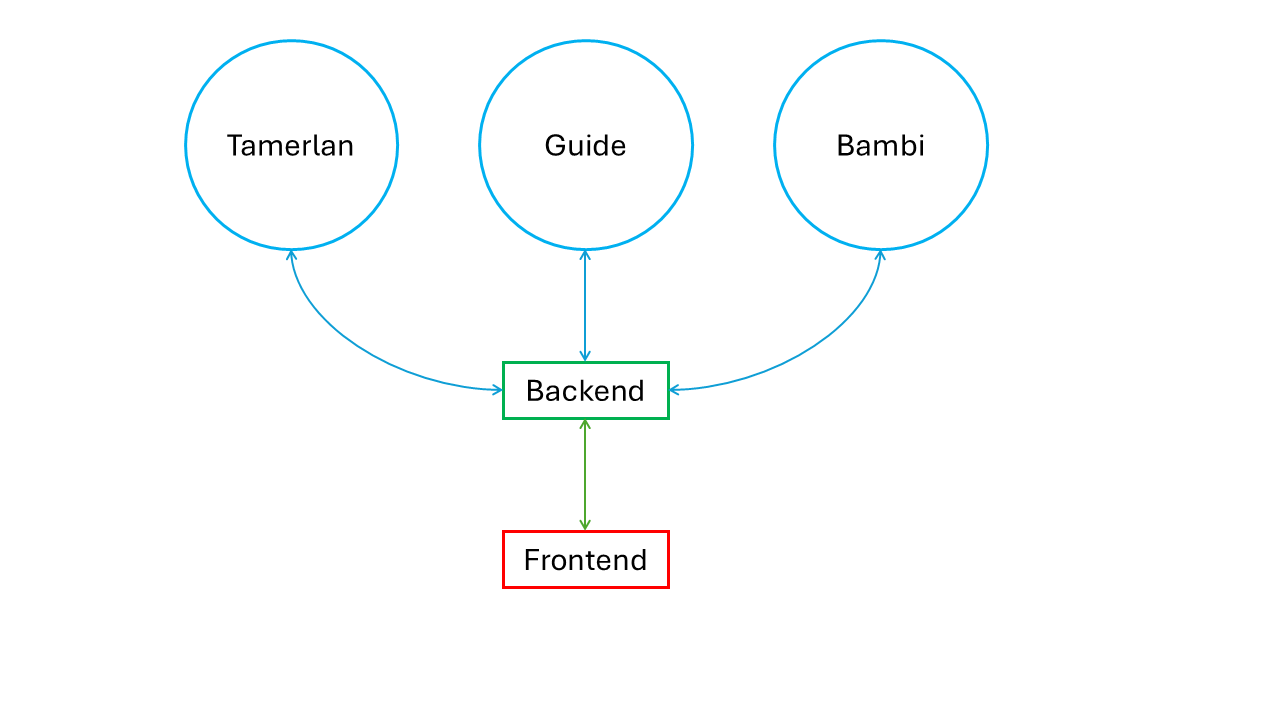
\includegraphics[width=\textwidth, center]{img/Kommunikationswege.png}  
    \caption{Kommunikationswege}
    \label{fig:kommunikationswege}
\end{figure}

\section{WebSockets}
\label{sec:websockets}
\initials{LG}
WebSockets nach RFC6455 \cite{rfc6455} erlauben bidirektionale Kommunikation zwischen einem Client und einem Server.
%
Das WebSocket-Protokoll ist ein unabhängiges TCP-basiertes Verfahren;
seine einzige Beziehung zu HTTP besteht darin,
dass der WebSocket-Handshake als HTTP-Anfrage nach mit Antwort vom Typ
\texttt{101 Switching Protocols} nach RFC2616 \cite{rfc2616} interpretiert werden kann.
%
Standardmäßig verwendet das WebSocket-Protokoll Port 80 für normale WebSocket
Verbindungen und Port 443 für WebSocket-Verbindungen,
die mittels Transport Layer Security (TLS) verschlüsselt werden.
%
Dank des schon eben erwähnten HTTP-kompatiblen Handshakes
können auf dem selben Port sowohl HTTP- als auch WebSocket-Dienste zur Verfügung gestellt werden,
solange sich deren Pfad unterscheidet.
%
Natürlich muss hier die Serversoftware sowohl HTTP als auch WebSockets unterstützen.

Der große Vorteil von Websockets ist,
wie schon erwähnt,
der bidirektionale Informationsfluss:
%
Beide Verbindungsteilnehmer können ungefragt Informationen an den jeweils anderen Teilnehmer senden.
%
Bei HTTP müssen Informationen immer zuerst vom Client angefragt werden,
was insbesondere bei zeitkritischen Anwendungen wie Spielen,
Messenger-Apps,
oder eben bei der Fernsteuerung von Robotern von großen Vorteil ist.
%
Es ist zwar möglich,
mittels HTTP die Funktionalität von WebSockets anzunähern (long Polling),
jedoch gibt es dabei unter Anderem \cite{rfc6202} einen signifikant erhöhten Performance-Overhead%
\footnote{Bis zu einigen hundert Bytes,
  was im Kontext der SwarmBots ein Vielfaches des tatsächlichen Nachrichteninhalts ist.}
und erhöhte Komplexität.

In diesem Projekt werden WebSockets sowohl zur Kommunikation zwischen Robotern und Server,
als auch zwischen Frontend und Server verwendet.

\section{Protocol Buffers}
\label{subsec:ueberblick_protobufs}
\initials{LG}
Protocol Buffers \cite{protobufs} (``protobufs'') sind ein binäres Übertragungsformat,
welches von Google entwickelt und veröffentlicht wurde.
%
Gegenüber Datenformaten wie JSON und XML gibt es drei wesentliche Vorteile:
\begin{enumerate}
    \item Da Protocol Buffers auf Binärdaten anstatt von Text basieren,
    ist die Übertragung viel effizienter \cite{7765670}.
    %
    Insbesondere bei der Verwendung mit Mikrocontrollern ist das ein enormer Vorteil.

    \item Bei Protocol Buffers gibt es explizit definierte Datenstrukturen.
    %
    Diese Datenstrukturen sind (bei korrekter Verwendung) mit älteren Versionen rückwärts-kompatibel.

    \item Für wie Verwendung mit unterschiedlichen Programmiersprachen kann (und soll) man aus protobuf-Definitionen
    Wrapper-Bibliotheken generieren.
    %
    Diese Wrapper-Bibliotheken können ohne weiteren Aufwand direkt verwendet werden,
    um auf die Datenstrukturen zuzugreifen.
\end{enumerate}

\subsubsection{Effizienz}
\initials{LG}
Wie schon oben erwähnt erreichen Protocol Buffers,
insbesondere bei kleinen Nachrichten,
einen viel kleineren Overhead als textbasierte Formate wie JSON oder XML.
%
Als Beispiel hierfür soll eine Nachricht vom Typ \texttt{EncoderData} gelten:
%
Mittels Protocol Buffers wird eine solche Beispielnachricht wie folgt übertragen:
%
\begin{lstlisting}[label=lst:testnachricht-proto,caption=Testnachricht (Protobuf) in Hexadezimaldarstellung]
    0890013205082a109c12
\end{lstlisting}
So ist die Testnachricht im Protobuf-Format lediglich 10 Bytes lang!
%
Zum Vergleich ist die gleiche Nachricht im JSON-Format um einiges länger:
\begin{lstlisting}[label=lst:testnachricht-json,caption=Testnachricht (JSON) als formattierter String]
{
  "seq": 144,
  "msg": {
    "pulses": 42,
    "duration": 2332
  }
}
\end{lstlisting}
So wie in Listing \ref{lst:testnachricht-json} dargestellt,
werden 71 Bytes benötigt.
%
Da im JSON Leerzeichen ignoriert werden können,
ist es möglich, die Größe der Nachricht auf 51 Bytes zu reduzieren.
%
Das ist immer noch mehr als zehn mal so viel wie mit Protocol Buffers.

Der Unterschied in Nachrichtengröße ist stark von der Nachricht selbst abhängig;
Bei größeren Nachrichten schrumpft der Overhead von JSON,
und damit der ``Vorsprung'' von Protocol Buffers,
allerdings werden Protocol Buffers immer effizienter als JSON sein.
%
Zu beachten ist auch,
dass bei JSON die Länge der Variablennamen einen Einfluss auf die Nachrichtengröße hat.
%
Für dieses Beispiel wurden die Bezeichnungen \texttt{sequence} und \texttt{message} absichtlich auf
\texttt{seq} respektive \texttt{msg} abgekürzt,
um die Testbedingungen etwas fairer zu gestalten.
%
Bei Verwendung von WebSockets ist JSON mehr als adäquat,
jedoch führen die Ineffizienzen des Formats bei anderen Protokollen,
wie ESP-NOW \cite{esp-now} (welches nur Nachrichten mit bis zu 250 Bytes unterstützt),
zu Problemen.
%
Um also die Möglichkeit zur Erweiterung auf andere Protokolle zu gewährleisten,
wurde auf die Vorteile von JSON verzichtet.

\subsubsection{Datenstruktur}
\initials{LG}
Die jeweiligen Nachrichten (``Payloads')
werden vom Nachrichtensender gemeinsam mit einer Sequenznummer in einem \texttt{Wrapper} verpackt,
welcher dann über die WebSocket-Verbindung an den Nachrichtenempfänger übertragen wird.
%
Der Empfänger speichert immer die letzte empfangene Sequenznummer,
und verwirft Nachrichten,
welche eine niedrigere Sequenznummer als die gespeicherte haben.
%
Eigentlich ist dies aufgrund der Verwendung von WebSockets nicht nötig,
da TCP-Pakete aufgrund einer eigenen Sequenznummer immer garantiert in der richtigen Reihenfolge ankommen.
%
Um die Verwendung des Protokolls mit anderen unterliegenden Transporten,
wie zum Beispiel UDP oder ESP-NOW,
zu erlauben,
wurde zusätzlich die protokolleigene Sequenznummer implementiert.
%
Genaue Informationen zum Datenformat können in Abschnitt
\ref{lstsec:incl-protobuf} auf Seite
\pageref{lstsec:incl-protobuf} gefunden werden.

\subsubsection{Wrapper-Bibliotheken}
\initials{LG}
Zur Verwendung von Protocol Buffers in Programmen gibt es eine Vielzahl von Wrapper-Bibliotheken,
welche es ermöglichen,
mit dem in den \texttt{.proto}-Dateien definiertem Format
Nachrichten zu erstellen und zu verarbeiten.
%
Da in diesem Projekt mehrere Programmiersprachen angewendet wurden,
wurden für die einzelnen Programme natürlich auch unterschiedliche Bibliotheken verwendet:
%
Für die Implementierung der Roboter in C++ wurde die Bibliothek \texttt{Nanopb} verwendet,
welche insbesondere für die Verwendung in Systemen mit limitierten Ressourcen gedacht ist.
%
Im Server wurde die Python-Bibliothek \texttt{protobuf} verwendet,
während am Frontend \texttt{protobufjs} mit eingebautem TypeScript-Support angewandt wurde.

Zur automatischen Generierung der Dateien zur Verwendung von Protobufs in der jeweiligen Programmiersprache
wurden von Herrn Gastgeber zwei kleine Skripten für die Roboter und das Frontend entwickeln,
welche bei Bedarf die jeweiligen Bibliotheksfunktionen aufrufen.
%
Beim Server ist leider das Ausführen eines Befehls und die manuelle Modifikation einer Datei notwendig,
wie in der Datei \texttt{server/README.md} dokumentiert. (Siehe Abschnitt \ref{lstsec:incl-server} auf Seiten \pageref{lstsec:incl-server}ff) 

\section{Sensoren}
\label{subsec:ueberblick_sensors}

\subsection{LiDAR}
\label{subsec:ueberblick_lidar}

\subsection{Gyroskop}
\initials{LG}
Jeder der drei Roboter ist mit einem Gyroskop/Accelerometer vom Typ \texttt{MPU6050} ausgestattet.
%
Dieser Sensor ist bereits im originalen Tumbller-Kit inkludiert, also ist die Installation entsprechend einfach.
%
Der \texttt{MPU6050} versorgt den Mikrocontroller über I2C mit Messdaten zu drei Gyroskop- und drei Accelerometerachsen.
%
Diese Informationen werden dann vom Mikrocontroller verwendet, um den Roboter aufrecht zu halten.
%
Weiters leitet der Mikrocontroller die Daten zur weiteren Verarbeitung bzw. Analyse für Debugging-Zwecke an den zentralen Server weiter.

\subsection{Drehgeber}
\label{subsec:ueberblick_rot_enc}
\initials{LG}
In den im Tumbller-Kit mitgelieferten Motoren ist bereits ein Drehgeber mit eingebaut,
welcher mit Hall-Sensoren funktioniert.
%
Mit diesem Drehgeber kann die aktuelle Motorgeschwindigkeit als Feedback zur Motorsteuerung gemessen werden.
%
Die Impulse des Drehgebers werden auf eine gewisse Zeitspanne im Format zusammengefasst und dann regelmäßig an den Server weitergeleitet.
	% Alles zur Hardware und unseren Modifikationen
% Zuständig: Mihael
\chapter{Hardware}
\label{sec:hardware}
\section{Elegoo Tumbller Kit}
\label{subsec:elegoo_tumbller}
Um den Hardwareaufbau so einfach wie möglich zu gestalten,
entschieden wir uns dafür,
fertig entwickelte Kits online zu bestellen und dann zu modifizieren.
%
Die Wahl des Kits fiel letztendlich auf den ``Tumbller'' von Elegoo (Siehe Abbildung \ref{fig:elegoo_tumbller}).
%
Der Tumbller ist ein zweirädriger Roboter, welcher auf einer Ache balanciert.
%
Zur Kontrolle des unmodifizierten Kits gibt es eine Smartphone-App,
welche die Roboter über Bluetooth fernsteuern kann.
%
Da wir die Roboter über WLAN steuern wollten, 
und die Tumbller-Kits standardmäßig nur eine Bluetooth-Erweiterung eingebaut haben,
haben wir die mitgelieferten Arduino Nano durch ESP32-Boards im Arduino Nano-Format ersetzt.
% TODO Spannungsunterschiede Arduino Nano vs ESP
\begin{figure}[H]
    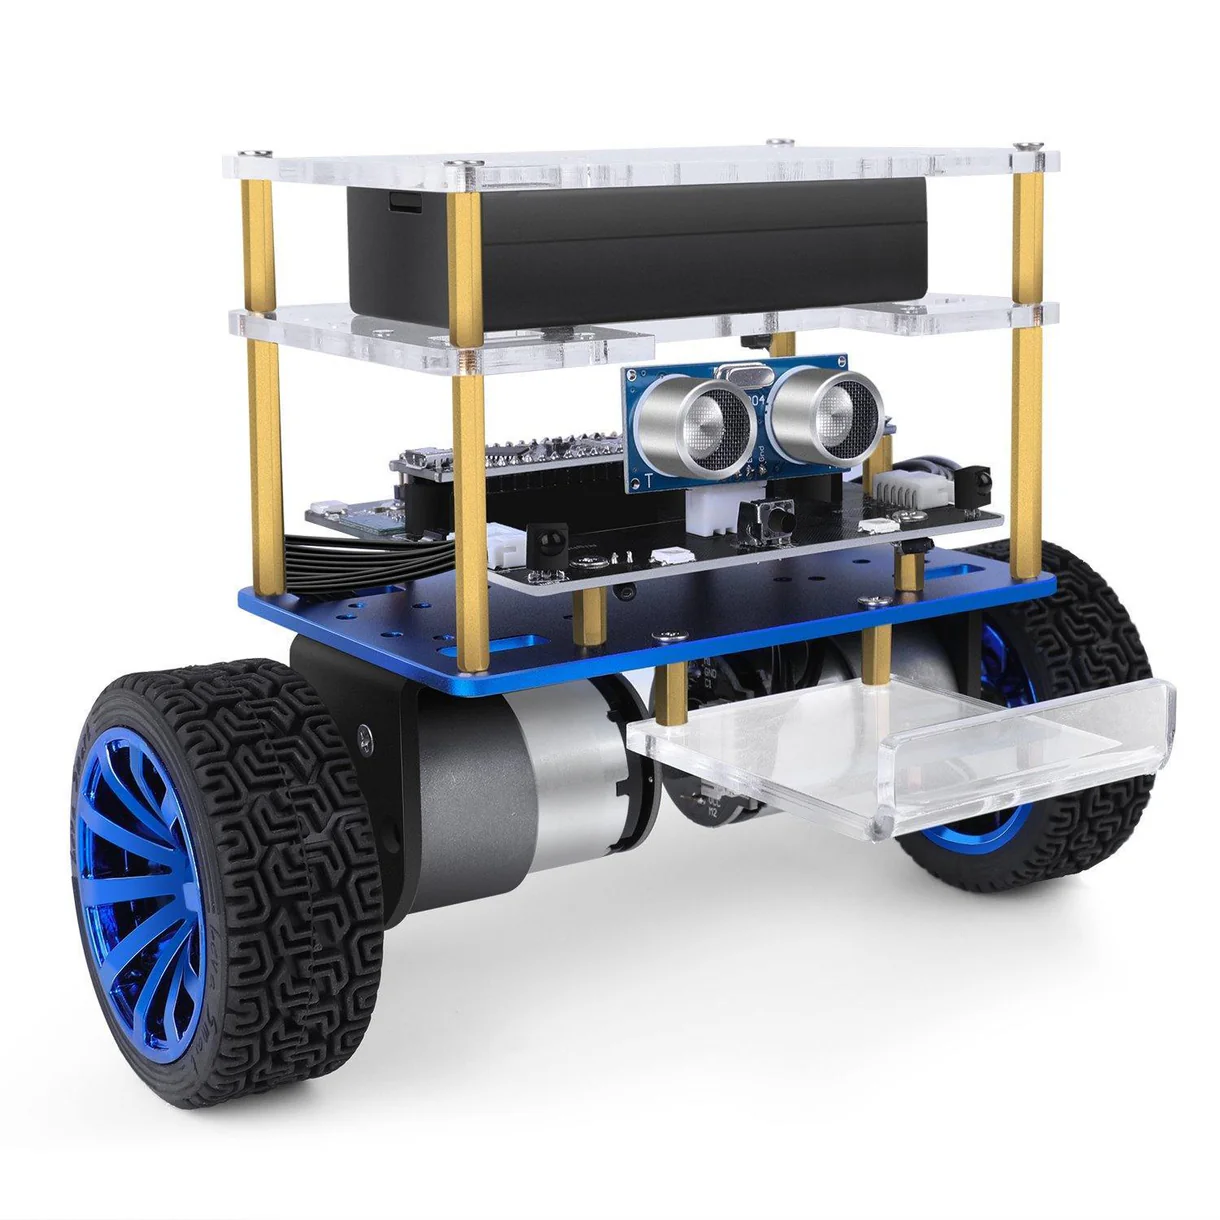
\includegraphics[width=0.7\textwidth, center]{img/elegoo_tumbller.png}
    \caption{Rendering des Elegoo Tumbller}
    \label{fig:elegoo_tumbller}
\end{figure}

Der unmodifizierte Elegoo Tumbler besteht aus einem Arduino Nano der zur Steuerung des gesamten Roboters verwendet wird. 
Einem MPU6050 (Gyroskop- \& Beschleunigungssensor), der zur Erkennung der Achsen und Bewegungen verwendet wird (balancieren). 
Des Weiteren hat er auch zwei Gleichstrommotoren mit Hall-Encodern zur Messung der Raddrehung, diese Motoren werden mit dem TB6612FNG Motortreiber gesteuert. 
Zudem verfügt der Elegoo Tumbler über ein HC-06 Bluetooth-Modul, das zur Kommunikation mit dem Smartphone verwendet wird. Mithilfe des SR04 Ultraschallsensor ist der Roboter in der Lage, 
Abstände zu messen, was es ihm ermöglicht, Hindernisse zu erkennen und zu umgehen.  
Zudem besitzt der Tumbler Infrarot-Sensoren (IR204C-A und IRM-56384), die es ihm ermöglichen, Hindernisse und Linien zu erkennen oder zu verfolgen. 
Durch den AMS1117 3.3V Spannungswandler wird die Spannung von dem Li-Ion-Akku, der als Hauptstromversorgung dient, heruntergestuft, 
sodass sie auch für das Bluetooth-Modul und die Sensoren verwendbar ist. Des Weiteren ist der Elegoo Tumbler mit mehreren Modi ausgestattet. 
Diese kann man entweder über die App oder direkt am Roboter über einen Taster steuern, zur Visualisierung der Modi hat der Elegoo Tumbler mehrere LEDs eingebaut.
\section{Subkomponenten}
\label{subsec:subkomponenten}
%
\subsection{PCB}
%
\subsubsection{Allgemein}
Die PCB (Printed Circuit Board) im originalen Elegoo Tumbller ist eine fertig entwickelte Leiterplatte, auf der alle elektronischen Bauteile des Roboters angeschlossen werden können.
Sie ist das zentrale Verbindungselement zwischen Sensoren, Motoren, Mikrocontroller und Stromversorgung.
Alle Bauteile müssen nur noch in die vorgefertigten Stecker und Buchsen eingesteckt werden. Dadurch ist der Aufbau des Roboters sehr einfach und es sind keine aufwändigen Lötarbeiten notwendig.
\subsubsection{Technische Umsetzung}
Die Leiterplatte besteht aus mehreren Leiterbahnen (Kupferstreifen), die die elektrische Verbindung zwischen den Bauteilen herstellen.
Die PCB enthält unter anderem:
\begin{itemize}
    \item Steckplätze für den Arduino Nano
    \item Anschlussbuchsen für die beiden Motoren
    \item Steckplätze für die Sensoren (MPU6050, Ultraschallsensor, Infrarot-Sensoren)
    \item Anschluss für das Bluetooth-Modul (HC-06)
    \item Taster für die Modus-Auswahl
    \item LEDs zur Anzeige des Betriebszustands
    \item Lötpads für die Stromversorgung (Li-Ion Akku)
    \item Anschluss für den AMS1117 Spannungsregler
\end{itemize}

Außerdem sind die Leiterbahnen so angeordnet, dass die Stromversorgung über die PCB zu allen Bauteilen geführt wird.
Die PCB hat ebenfalls Lötpunkte für die Motorsteuerung (TB6612FNG Motortreiber), der direkt auf der Platine verlötet ist.
\subsubsection{Vorteile}
Die originale PCB im Elegoo Tumbller hat mehrere Vorteile: 
\begin{itemize}
    \item Einfacher Aufbau → Alle Komponenten können einfach eingesteckt werden
    \item Ordentliche Verkabelung → Keine losen Kabel
    \item Platzsparend und kompakt → Alles ist auf einer Platine montiert
    \item Stabile Verbindung → Weniger Wackelkontakte
    \item LEDs zur Anzeige des Betriebszustands  
\end{itemize}

\subsubsection{Einschränkungen}

Die PCB des originalen Tumbller ist nur für die Standard-Komponenten ausgelegt.
Wenn man zusätzliche Sensoren oder einen anderen Mikrocontroller (wie im SwarmBots-Projekt) verwenden möchte, muss die Verkabelung angepasst oder die Platine teilweise umgelötet werden.
Außerdem ist sie nicht flexibel, wenn man den Aufbau verändern will.

%
Siehe Abbildung \ref{fig:elegoo_tumbller_original_circuit} auf Seite \pageref{fig:elegoo_tumbller_original_circuit}.
%
\begin{sidewaysfigure}
    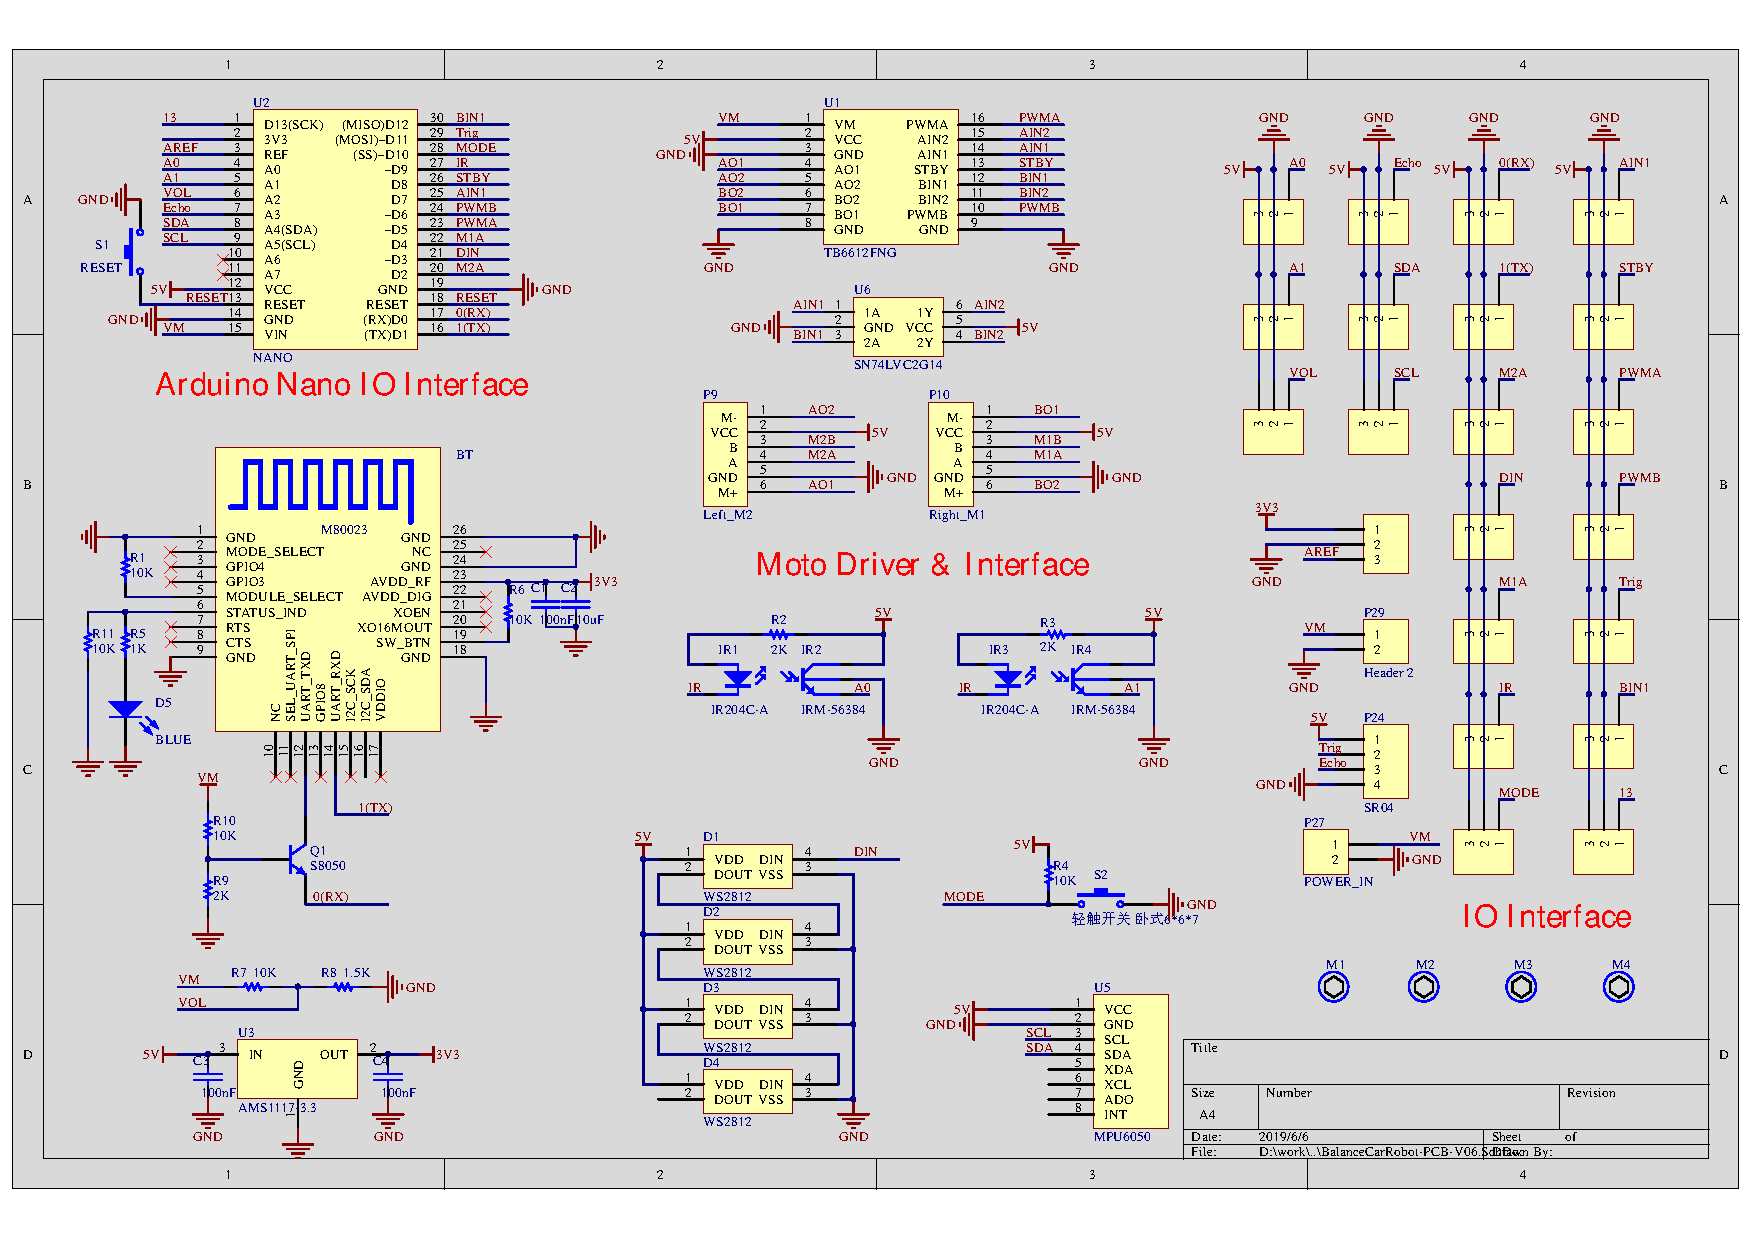
\includegraphics[width=\textwidth, center]{img/elegoo_tumbller_original_circuit.pdf}
    \caption{Originaler Schaltplan des Tumbllers (TODO: neu zeichnen)}
    \label{fig:elegoo_tumbller_original_circuit}
\end{sidewaysfigure}
%
\subsection{MPU6050 (Gyroskop- \& Beschleunigungssensor)}
%
\subsubsection{Allgemein}
Der MPU6050 ist ein 6-Achsen-Sensor, der aus einem Drehratensensor (Gyroskop, welcher Drehbewegungen in 3 Achsen) und 
einem Beschleunigungssensor (Accelerometer, welcher lineare Beschleunigungen in 3 Achsen misst).
\subsubsection{Technische Daten}
\begin{figure}[H]
    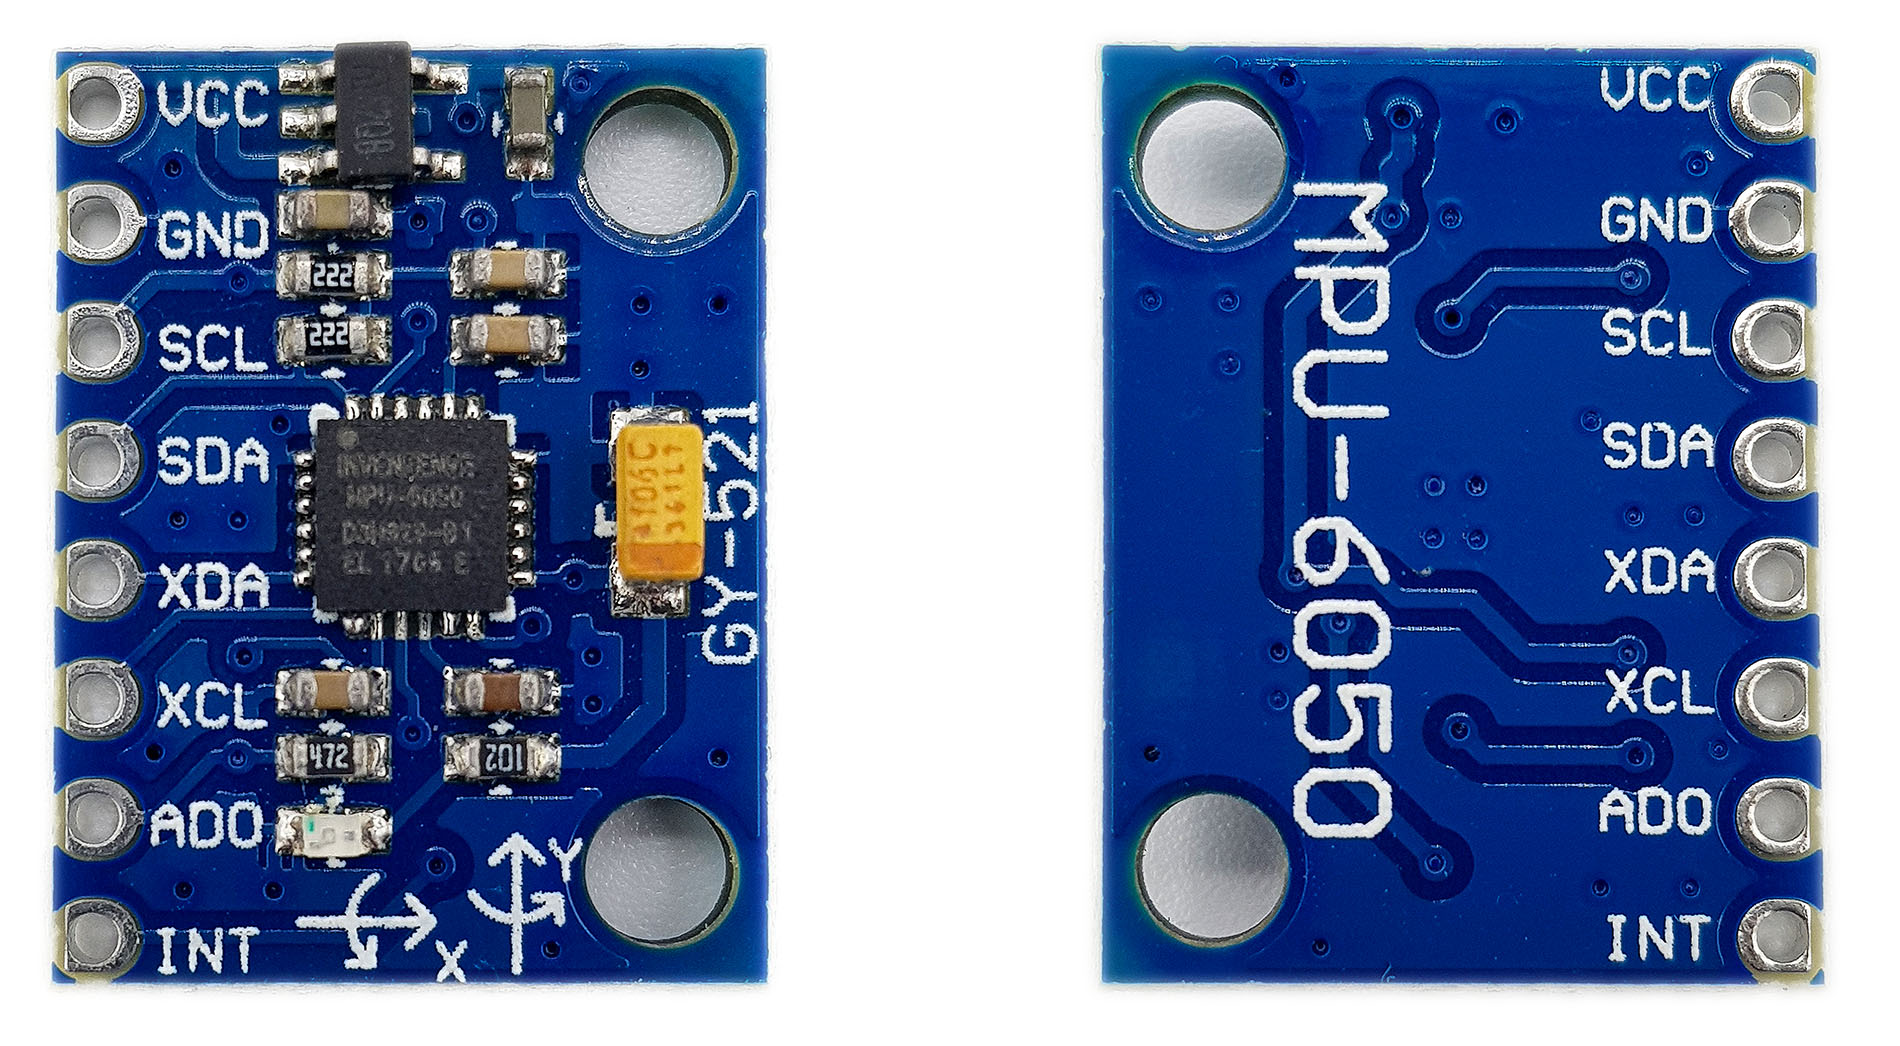
\includegraphics[width=0.7\textwidth, center]{img/Hardware/MPU6050.png}
\end{figure}
Als Betriebsspannung verwendet der MPU6050 2,3V bis 3,4V, als Kommunikationsprotokoll verwendet er I2C oder SPI (I2C Standard: 0x68 Adresse). 
Der Messbereich des Gyroskops und Accelerometers kann konfiguriert werden (Gyroskop:  ±250, ±500, ±1000, ±2000 °/s, Accelerometer: ±2g, ±4g, ±8g, ±16g), 
durch die Konfigurationsmöglichkeit ergeben sich auch unterschiedliche Empfindlichkeiten der beiden (Gyroskop: 131 LSB/°/s (bei ±250 °/s), 
Accelerometer: 16.384 LSB( least significant bit/ niedrigstes Bit)/g (bei ±2g)).  
Die Genauigkeit der beiden liegt bei ca. ±0,01 °/s für den Gyroskop-Sensor und ca. ±0,005g für den Accelerometer. 
Zudem verfügt der MPU6050 über eine Abtastrate von bis zu 1kHz und über einen integrierten DMP (Digital Motion Processor), welcher es ermöglicht, Datenfusion durchzuführen.
\subsubsection{Einschränkungen}
Der Gyroskop-Sensor hat einen Drift, der dazu führt, dass sich die Messwerte bei längerer Laufzeit verschieben. 
Zudem reagiert der MPU6050 empfindlich auf Vibrationen, wodurch Messfehler entstehen können.
%
\subsection{TB6612FNG (Motortreiber)}
%
\subsubsection{Allgemein}
Der TB6612FNG ist ein Dual-H-Brücke-Motortreiber, welcher verwendet wird, um einen Schrittmotor oder zwei Gleichstrommotoren wie beim Tumbler zu steuern. 
Der Motortreiber ermöglicht es, Gleichstrommotoren in zwei Richtungen zu betreiben.
\subsubsection{Technische Daten}
\begin{figure}[H]
    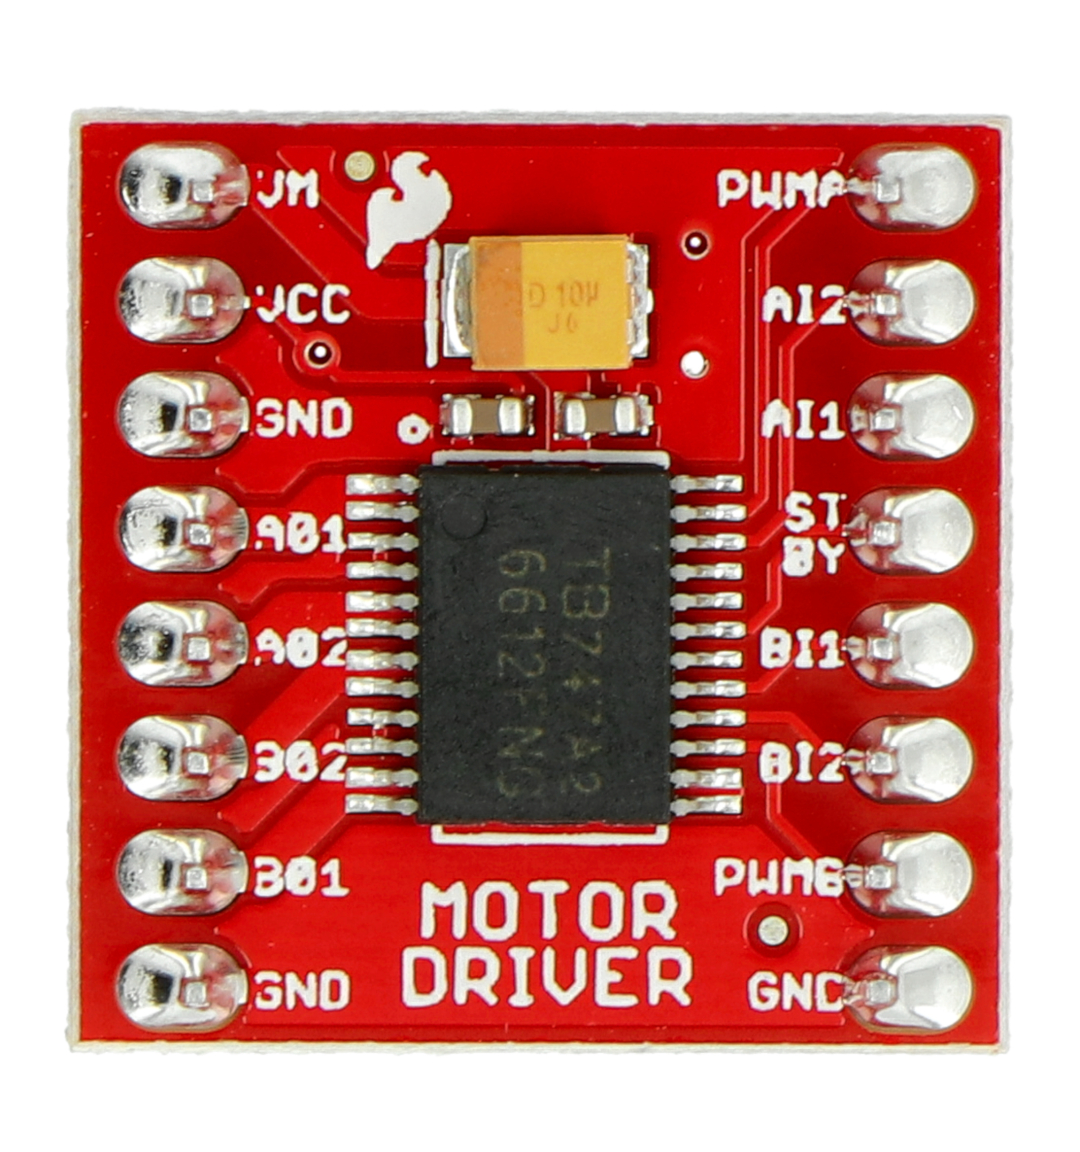
\includegraphics[width=0.3\textwidth, center]{img/Hardware/Motortreiber.png}
\end{figure}
Als Versorgungsspannung für Motoren kann der TB6612FNG 2,5V bis 13,5V ausgeben, für die Logik ist die Versorgungsspannung 2,7V bis 5,5V. 
Der maximale Ausgangsstrom ist 1,2 A (kontinuierlich), 3 A (kurzzeitig pro Kanal), er besitzt 2 Kanäle und als Steuersignal verwendet er PWM (Pulsweitenmodulation) und Richtungssignale. 
Zudem besitzt er eine integrierte Schutzschaltung, die vor Überstromschutz, Übertemperaturschutz und Kurzschlussschutz schützt. 
Die Verlustleistung ist sehr gering, da der Motortreiber die MOSFET-Technologie verwendet. (MOSFET (Metal Oxide Semiconductor Field Effect Transistor) ist ein elektronisches Bauteil, 
das wie ein elektronischer Schalter funktioniert und in der Motorsteuerung verwendet wird, um mit einem kleinen Steuersignal einen großen Stromfluss für Motoren zu kontrollieren)
\subsubsection{Belegung}
Pin	-	Funktion
VM	Versorgungsspannung für die Motoren (2,5–13,5V)
VCC	Logik-Spannungsversorgung (2,7–5,5V)
GND	Masse (gemeinsames Minus)
AIN1	Richtungssignal Motor A (Logik-Eingang)
AIN2	Richtungssignal Motor A (Logik-Eingang)
PWMA	PWM-Signal für Geschwindigkeit Motor A
BIN1	Richtungssignal Motor B (Logik-Eingang)
BIN2	Richtungssignal Motor B (Logik-Eingang)
PWMB	PWM-Signal für Geschwindigkeit Motor B
STBY	Standby-Pin (aktiv bei HIGH)
AO1	Ausgang Motor A (Pluspol)
AO2	Ausgang Motor A (Minuspol)
BO1	Ausgang Motor B (Pluspol)
BO2	Ausgang Motor B (Minuspol)

\subsubsection{Ansteuerung}
Durch die Kombination Richtungssignale (AIN1, AIN2 / BIN1, BIN2), kann der Motor entweder vorwärts-, rückwärtsfahren oder anhalten.
Der PWMA/PWMB sorg dafür, dass sich die Geschwindigkeit ändert.
%
\subsection{AMS1117 (3.3V Spannungsregler)}
%
\subsubsection{Allgemein}
Der AMS1117 ist ein linearer Spannungsregler, der aus einer höhere Eingangsspannung eine stabile kleinere Ausgansspannung (3,3V) macht. 
Im Elegoo Tumbller wird er verwendet, um die Spannung auf 3,3 Volt zu reduzieren. Diese Spannung brauchen einige Bauteile, wie zum Beispiel das Bluetooth-Modul, damit sie nicht kaputtgehen.
\subsubsection{Technische Daten}
\begin{figure}[H]
    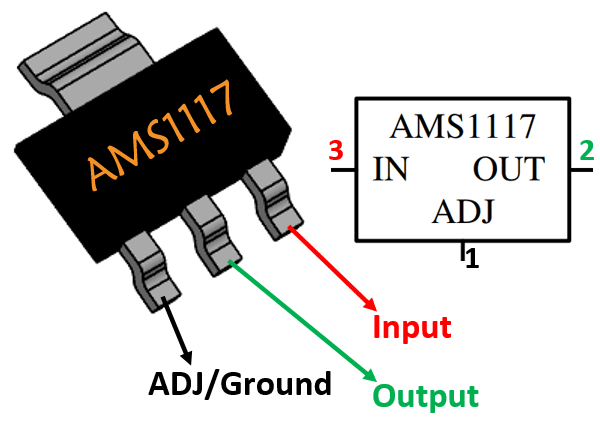
\includegraphics[width=0.6\textwidth, center]{img/Hardware/AMS1117.png}
\end{figure}
Der Spannungsregler kann mit 4,5V bis 15V betrieben werden, er hat eine fixe Ausgansspannung von 3,3V und kann maximal 1A Ausgangstrom liefern (mit einer Kühlung), 
die Drop-out Spannung beträgt 1,1V (bei 1A). der Integrierte Schutz schütz vor Übertemperatur und Kurzschlüssen.
%
\subsection{HC-06 (Bluetooth Modul)}
%
\subsubsection{Allgemein}
Das HC-06 ist ein Bluetooth Modul der es ermöglicht über eine kurze Distanz ohne Kabel daten zu übertragen. 
(Bluetooth ist eine Funktechnik, die Daten über kurze Distanzen per Funkwellen im 2,4-GHz-Band überträgt und dabei eine serielle, kabellose Verbindung zwischen zwei Geräten herstellt.)
\subsubsection{Technische Daten}
\begin{figure}[H]
    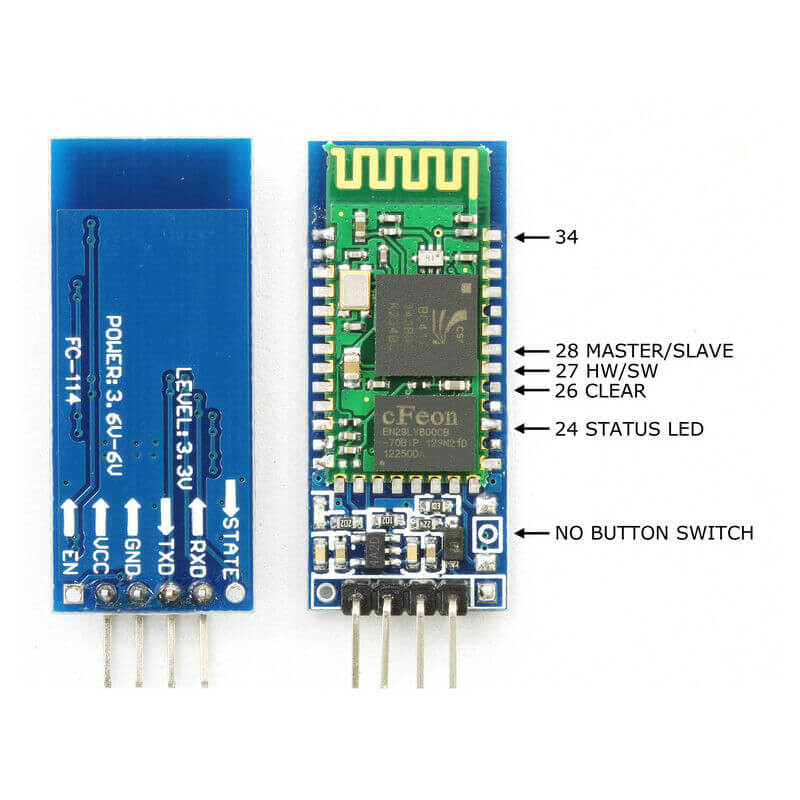
\includegraphics[width=0.6\textwidth, center]{img/Hardware/hc06.png}
\end{figure}
Das Bluetooth Modul wird mit einer Betriebsspannung von 3,3V betrieben als Kommunikationsmetode verwendet es UART 
(UART (Universal Asynchronous Receiver Transmitter) ist eine serielle Schnittstelle, die Daten bitweise und ohne Taktsignal zwischen zwei Geräten über nur zwei Leitungen (TX und RX) überträgt.).  
Die Version, die es unterschütz ist, Bluetooth 2.0 + EDR, es hat eine Reichweite von bis zu ca.  10m und hat eine Datenrate von bis zu 2,1 Mbps. 
Als Funkfrequenz verwendet es sdas 2,4 GHz Band, die Sicherheitsfunktion, die man einschalten kann, erfordert es einen Pin-Code vor der Verbindung einzugeben. 
Das HC-06 ferfügt nur über den Slave-Modus. 
(Der Slave-Modus bedeutet, dass ein Gerät keine Verbindung selbst starten kann, sondern nur auf Verbindungsanfragen von anderen Geräten wartet und dann darauf reagiert.)
\subsubsection{Belegung}
Pin	-	Funktion
VCC	Versorgungsspannung (3,3V)
GND	Masse
TXD	Sendedaten (wird mit RX des Arduino verbunden)
RXD	Empfangsdaten (wird mit TX des Arduino verbunden)
STATE	Verbindungsstatus-Ausgang (optional)

\subsubsection{Einschränkungen}
Durch die veraltete Bluetooth-Version ist nur eine niedrigere Datenrate möglich und es besteht eine höhere Störanfälligkeit als bei modernen Standards.
%
\subsection{Arduino Nano (Microcontroller)}
%
\subsubsection{Allgemein}
Der Arduino Nano ist einer der kleineren (ca. 18 x 45 mm) uC (Mikrocontroller), dieser wurde verwendet, um alle elektronischen Bauteile im Tumbler zu steuern.
\subsubsection{Technische Daten}
\begin{figure}[H]
    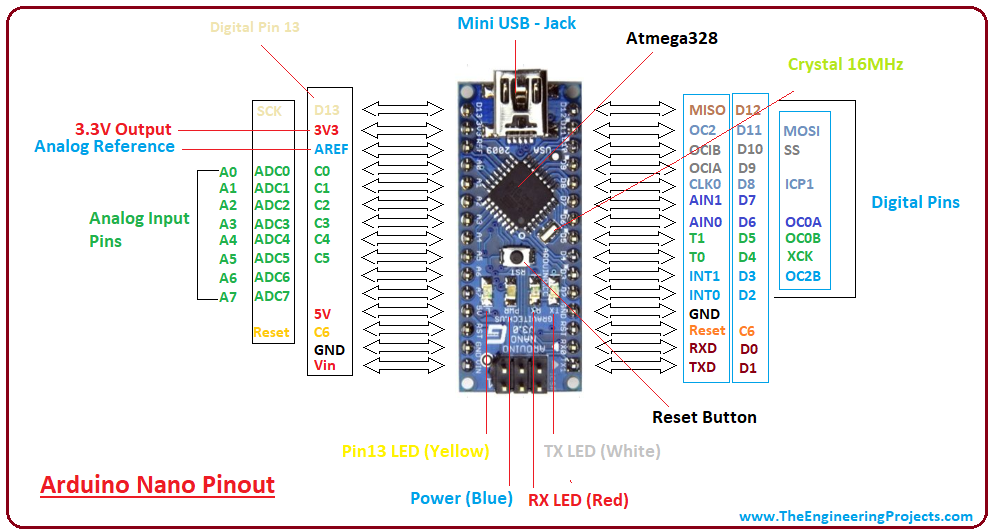
\includegraphics[width=1\textwidth, center]{img/Hardware/arduino_nano.png}
\end{figure}
Der Arduino Nano hat einen ATmega328P als Prozessor und eine Taktfrequenz von 16MHz. Die Betriebsspannung beträgt 5V (Versorgungspannung über den Pin VIN 7V bis 12V). 
er besitz 14 Digitale i/O Pins (Input/Output), wobeit 6 davon PWM fähig sind. Zudem besitz er 8 Analoge Pins und einen Flash-Speicher von 32KB (davon 2 KB für Bootloader). 
Der SRAM hat 2KB und das EEPROM 1KB. Die Schnittstellen, die er unterschützt, sind UART, I2C, SPI.
UART (Universal Asynchronous Receiver Transmitter)
UART ist eine serielle Schnittstelle, die Daten bitweise über zwei Leitungen (TX für Senden und RX für Empfangen) überträgt. 
Dabei wird kein Taktsignal verwendet – beide Geräte müssen die gleiche Geschwindigkeit (Baudrate) eingestellt haben.
I2C (Inter-Integrated Circuit)
I2C ist ein Kommunikationsprotokoll, das mehrere Geräte über nur zwei Leitungen verbindet: eine Datenleitung (SDA) und eine Taktleitung (SCL). 
Ein Gerät ist der Master (Steuergerät), die anderen sind Slaves (empfangen Befehle).
SPI (Serial Peripheral Interface)
SPI ist eine serielle Schnittstelle für den schnellen Datenaustausch zwischen einem Master und einem oder mehreren Slave-Geräten. 
Es werden vier Leitungen verwendet: MOSI (Daten vom Master zum Slaven), MISO (Daten vom Slave zum Master), SCK (Taktsignal) und SS (Slave Select, Auswahl des Geräts).
\subsubsection{Belegung}
(Bild)
\subsubsection{Einschränkungen}
Der Arduino-Nano besitzt ein kleiner Speicher was ihn  nicht geeignet macht für komplexen Programmen, die viel Speicher benötigen. 
Zudem hat er nur einen 8-Bit-Prozzesor, was ihn auch in der Rechenleistung stark begrenzt. Desweitern hat er kein integriertes WLAN-Modul, 
was es nur ermöglicht ihn  über Kabel oder Bluetooth zu verwenden.
%
\subsection{SR04 (Ultraschallsensor)}
%
\subsubsection{Allgemein}
Der SR04 ist ein Ultraschallsensor, der verwendet wird, um den Abstand zu Objekten zu messen. 
Er sendet einen Ultraschallton aus, dieser wird von einem Hindernis reflektiert, und der Sensor misst die Zeit, bis das Echo zurückkommt.
\subsubsection{Technische Daten}
\begin{figure}[H]
    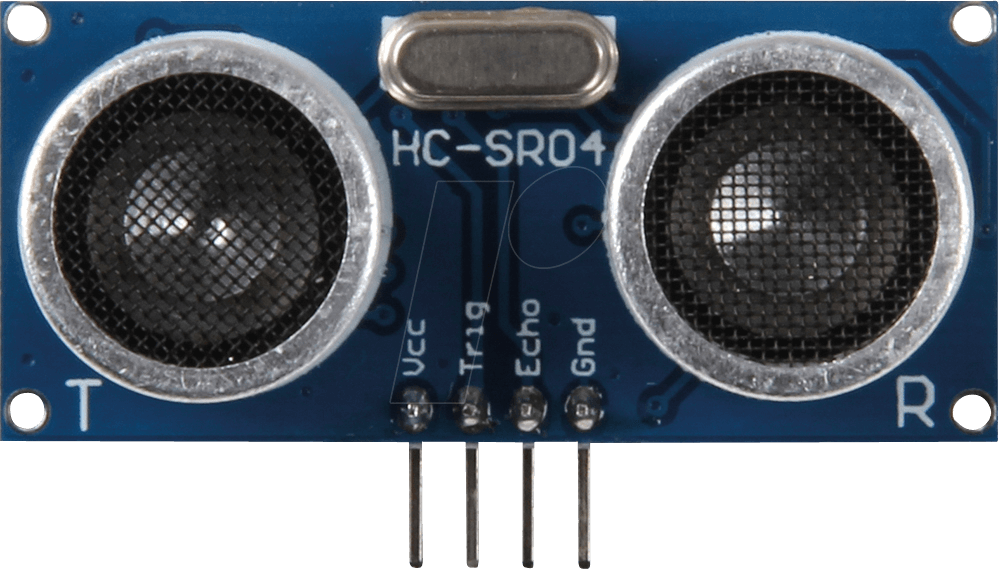
\includegraphics[width=0.7\textwidth, center]{img/Hardware/sr04.png}
\end{figure}
Der SR04 hat eine Betriebsspannung von 5V und eine Stromaufnahme von ca. 15mA. 
Zudem hat er einen Messbereich von 2cm bis 400cm und eine Genauigkeit von ca. ±3 mm. 
Sein Messwinkel beträgt 15° und er hat als Ausgänge den Trigger-Pin (Signal senden) und Echo-Pin (Signal empfangen). 
Die Frequenz mit der er arbeitet, sind 40 kHz (Ultraschall).
\subsubsection{Belegung}
Pin  -   	Funktion
VCC	Versorgungsspannung (5V)
GND	Masse
Trig	Trigger-Eingang → Startet das Signal
Echo	Echo-Ausgang → Gibt das empfangene Signal weiter
\subsubsection{Einschränkungen}
Der Ultraschall Sensor ist sehr empfindlich gegenüber schrägen Flächen und arbeitet relativ Langsam was ihn ungeeignet mach für bestimmte Orte und aufgaben. 
Zudem kann er bei Objekten unter 2cm Entführung keine Messung machen.
%
\subsection{Infrarot-Sensoren (IR204C-A \& IRM-56384)}
%
\subsubsection{Allgemein}
Die Infrarot-Sensoren IR204C-A und IRM-56384 werden im Elegoo Tumbller verwendet, um Hindernisse und Linien zu erkennen.
Sie funktionieren mit unsichtbarem Infrarotlicht (kurz: IR) und arbeiten nach dem Reflexionsprinzip.
\subsubsection{Technische Daten}
\begin{figure}[H]
    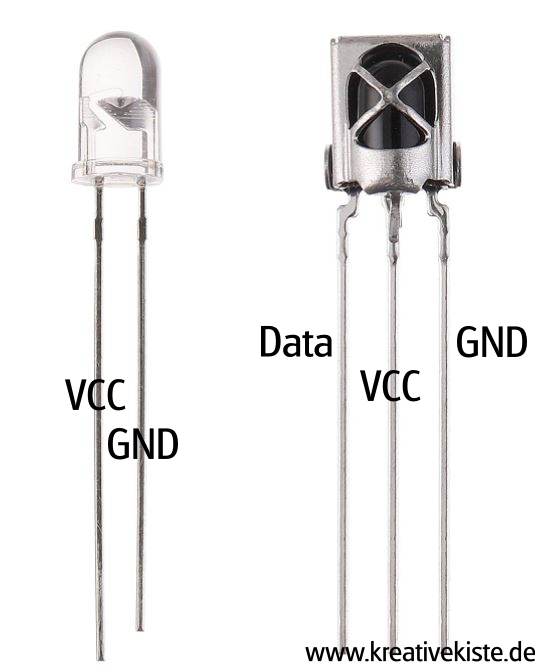
\includegraphics[width=0.4\textwidth, center]{img/Hardware/Infrarot_Sensor.png}
\end{figure}
Die Infrarot Sensoren arbeiten mit einer Betriebspannung von 5V und bestehen aus einer Infrarot-LED (LED, welche Infrarot Licht ausstrahlt) und 
einem Fototransistor (Transistor, welcher auf Licht reagiert). 
Der Erfassungsbereich liegt bei ca. 1 cm bis 10 cm (je nach Oberfläche), als Ausgang hat es Digital (HIGH = frei, LOW = Hindernis erkannt). 
Die Wellenlänge, mit welcher es arbeitet ist ca. 940 nm (unsichtbares Infrarotlicht).
IR204C-A:
Der IR204C-A ist eine Infrarot-LED. Sie sendet unsichtbares Infrarotlicht aus. 
Dieses Licht wird von Objekten reflektiert, damit der Roboter erkennen kann, ob ein Hindernis vor ihm steht.
IRM-56384:
Der IRM-56384 ist ein Infrarot-Empfänger. Er empfängt Infrarot-Signale und erkennt, ob Licht von der Infrarot-LED zurückkommt oder ob ein Signal von einer Fernbedienung gesendet wird.
\subsubsection{Einschränkungen}
Da die Infrarot LED nicht stark ist  und der Empfänger nicht genau kann es zu Problemen führen bei Tageslicht oder Lampen. 
Zudem funktionier diese Verfahren nur auf sehr kurzer Distanz (meist unter 10cm), und das Material welcher als Reflektor dient, kann ein Problem aufweisen da, 
Schwarze oder matte Flächen schlechter reflektieren.
%
\subsection{Gleichstrommotoren (TT130 DC Motor mit 1:48 Getriebe)}
%
\subsubsection{Allgemein}
Im Elegoo Tumbller werden zwei kleine Gleichstrommotoren (DC-Motoren) verwendet.
Diese Motoren sind dafür verantwortlich, die beiden Räder des Roboters anzutreiben.
Ein Gleichstrommotor wandelt elektrische Energie in mechanische Bewegung um – also in eine Drehbewegung.
\subsubsection{Technische Daten}
\begin{figure}[H]
    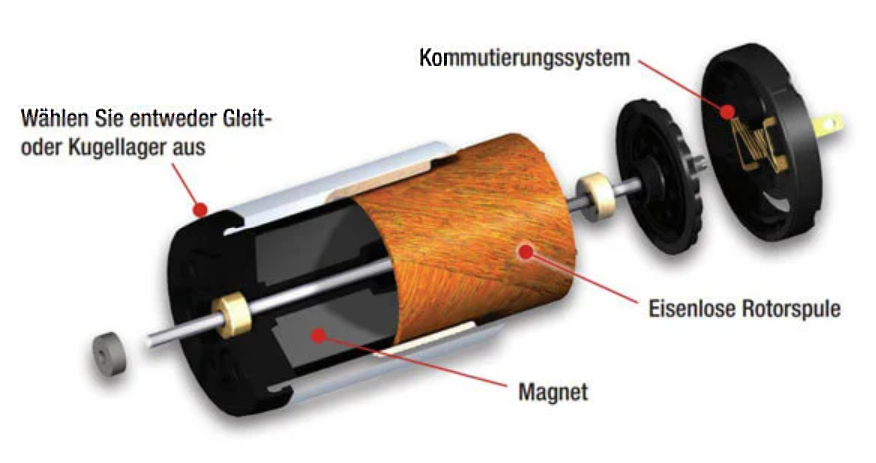
\includegraphics[width=1\textwidth, center]{img/Hardware/gleichstrommotor.png}
\end{figure}
Die Gleichstrommotoren haben eine Betriebsspannung von 6V bis 12V und einen Nennstrom von ca. 200mA und sind Bürsten-Gleichstrommotor. 
(Ein Bürsten-Gleichstrommotor ist ein Motor, der mithilfe von kleinen Bürsten Strom bekommt und sich dadurch dreht) Die Drehzahl beträgt ca. 300 Umdrehungen pro Minute (RPM). 
Zudem verfügen sie über ein eingebautes Getriebe zur Erhöhung des Drehmoments und einen Wellen-Durchmesser von 3mm. 
(Das Drehmoment gibt an, wie stark er etwas drehen kann, der Wellen-Durchmesser beschreibt, wie dick die Achse des Motors is)
\subsubsection{Funktionsweise}
Bei einem Gleichstrommotor wird durch Anlegen einer elektrischen Spannung ein Magnetfeld erzeugt, welches den Rotor bewegt. 
Durch Umpolen (Richtungsänderung des Stroms) kann die Drehrichtung geändert werden. 
Die Geschwindigkeit wird durch PWM-Signale (Pulsweitenmodulation) geregelt, die Richtung durch digitale Signale.

%
\subsection{Encoder}
%
\subsubsection{Allgemein}
Die Encoder im Elegoo Tumbller sind in den Motoren eingebaut und dienen dazu, die Drehbewegung der Räder zu messen.
Ein Encoder ist ein kleiner Sensor, der erkennt, wie weit und wie schnell sich ein Rad dreht. 
Damit kann der Roboter berechnen, wie viel Strecke er zurückgelegt hat oder wie stark sich das Rad gedreht hat – das ist wichtig für die Stabilität, Steuerung und Navigation.
\subsubsection{Technische Daten}
\begin{figure}[H]
    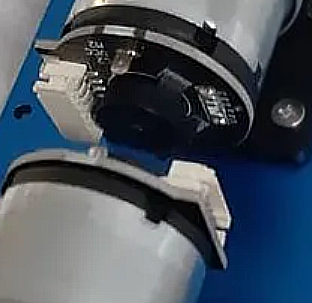
\includegraphics[width=0.6\textwidth, center]{img/Hardware/encoder.png}
\end{figure}
Die Encoder sind Magnetische Inkremental-Encoder sie arbeiten mit Digitalen Impulssiganlen und haben eine Impulszahl von ungefähr 11 Impulsen pro Rad-Umdrehung. 
Sie werden mit 5V betrieben und sind direkt am Motor befestigt. 
\subsubsection{Funktionsweise}
Am Motor ist ein kleiner Magnet eingebaut, der sich mit dreht, der Hallsensor erkennt jedes Mal, wenn der Magnet eine bestimmte Stelle passiert, 
wenn das der Fall ist wird ein elektrischer Impuls gesendet, dieser Impuls wird von dem Microcontroller dann gezählt.
\subsubsection{Funktionsweise}
Dadurch das die Encoder aber nur ca. 11 Impulse pro Umdrehung schaffen, ist keine genaue Steuerung Möglich. 
Zudem erkenne sie nur relative Bewegungen und keine Absoluten.
%
\subsection{Li-Ion Akku (7,4V)}
%
\subsubsection{Allgemein}
Der Li-Ion Akku (Lithium-Ionen-Akku) ist die Hauptstromquelle des Roboters. 
Er liefert die elektrische Energie, die der Roboter benötigt, um alle Komponenten wie Motoren, Sensoren und den Mikrocontroller zu betreiben.
\subsubsection{Technische Daten}
Beim Akku handelt es sich um einen Lithium-Ionen-Akku mit einer Nennspannung von 7,4V. 
Der Akku besitz je 2 Zellen in Serie (2S) mit je Zelle ca. 3,7V, die Kapazität des Akkus beträgt ca. 1200 mAh. Zudem ist er gegen Überladung, Tiefentladung und Kurzschlüsse geschützt. 
%

\section{Modifikationen}
\label{subsec:hardware_modifikationen}
Für das SwarmBots-Projekt mussten die originalen Elegoo Tumbller Roboter technisch verändert werden, damit sie als Schwarm zusammenarbeiten können und über WLAN steuerbar sind.
\subsubsection{Austausch des Mikrocontrollers}
Im originalen Tumbller wurde ein Arduino Nano verwendet, der jedoch nur Bluetooth-Kommunikation unterstützt.
Für unser Projekt war das nicht ausreichend, weil wir die Roboter über WLAN steuern wollten.
Deshalb haben wir die Arduino Nano durch ESP32-Boards im Nano-Format ersetzt.
Das ESP32-Board besitzt ein integriertes WLAN-Modul und mehr Rechenleistung.
\begin{figure}[H]
    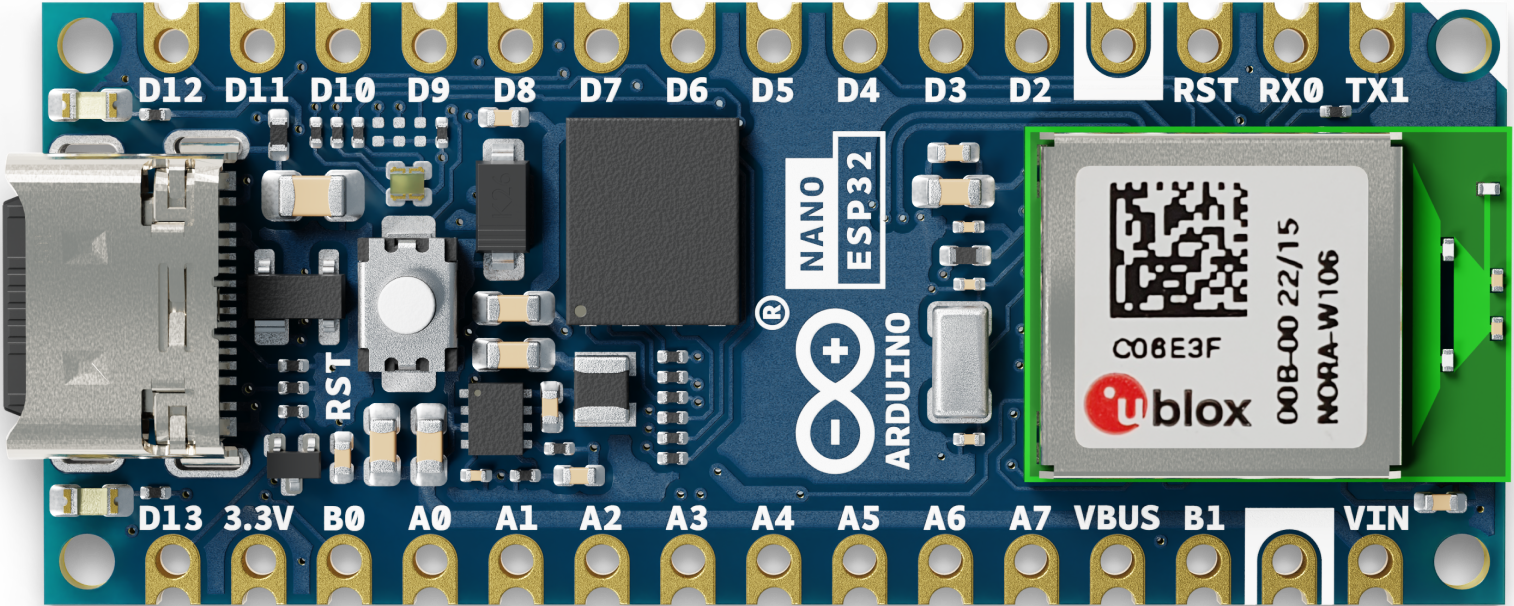
\includegraphics[width=0.6\textwidth, center]{img/Hardware/nanoesp32.png}
\end{figure}
\subsubsection{Entfernung des Bluetooth-Moduls}
Da wir die Kommunikation über WLAN umgestellt haben, wurde das HC-06 Bluetooth-Modul aus allen Robotern entfernt.
Die Steuerung per Smartphone-App war dadurch nicht mehr notwendig.
\subsubsection{Anpassung der Stromversorgung}
Für die neuen Module (vor allem den LiDAR-Sensor beim Guide-Roboter) musste die Stromversorgung angepasst werden.
Dafür haben wir einen zusätzlichen Step-Down-Konverter eingebaut, um eine sichere 5V-Spannung für den Sensor bereitzustellen.
\begin{figure}[H]
    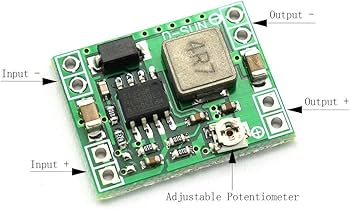
\includegraphics[width=0.6\textwidth, center]{img/Hardware/stepdown.png}
\end{figure}
\subsubsection{Mechanische Änderungen am Guide}
Der Guide-Roboter bekam zusätzlich einen LiDAR-Sensor auf der obersten Ebene montiert.
Dafür wurde das Chassis verändert:
\begin{itemize}
    \item Die obere Ebene wurde erhöht
    \item Neue Halterungen für den Sensor wurden eingebaut
    \item Das Kabelmanagement wurde angepasst
\end{itemize}



% Kamera-Integration (ESP32-CAM)
%Alle Roboter wurden mit einem ESP32-CAM-Modul ausgestattet.
% Dadurch können die Roboter Live-Bilder an den Server senden und ihre Umgebung visuell erfassen.



\section{Guide}
\label{subsec:hardware_guide}
\subsection{Allgemein}
Die Aufgabe von \textit{Guide} ist es,
mithilfe eines LiDAR-Sensors (Siehe Kapitel \ref{subsec:ueberblick_lidar}) die Umgebung nach Hindernissen
und den anderen Robotern abzusuchen.
%
\subsection{Technische Umsetzung}
Damit der Guide die Umgebung erkennen kann, wurde das Fahrgestell des Roboters modifiziert. Die obere Ebene (Akku-Halterung) wurde höher gesetzt, um Platz für den LiDAR-Sensor und seine Halterung zu schaffen. Zusätzlich wurde die Stromversorgung angepasst, indem ein Step-Down-Konverter eingebaut wurde. Dieser liefert die benötigte Spannung für den LiDAR-Sensor.
%
Die vom Guide gesammelten Daten werden über eine TCP/IP Websocket-Verbindung an einen zentralen Server gesendet. Dieser Server verarbeitet die Daten und teilt sie den anderen Robotern im Schwarm mit.
%
\subsection{Aufgabe im Schwarm}
Der Guide übernimmt die Funktion eines „Anführers“.
Er scannt ständig die Umgebung und erkennt:
\begin{itemize}
    \item Wände und Hindernisse
    \item Andere Roboter
    \item Freie Wege
\end{itemize}
Die anderen Roboter erhalten diese Informationen in Echtzeit und können dadurch ihre Bewegung anpassen.
Ohne den Guide könnten die Roboter keine Informationen über ihre Umgebung austauschen.
%
\subsection{Einschränkungen}
Da der Guide durch den zusätzlichen Sensor schwerer ist, hat er eine etwas kürzere Akkulaufzeit als die anderen Roboter. Außerdem ist der LiDAR-Sensor anfällig für Spiegelungen oder Glasflächen, weil die Laserstrahlen dort falsch reflektiert werden können.

%
\section{Tamerlan \& Bambi}
\label{subsec:hardware_tamerlan_bambi}

\subsection{Allgemein}
Tamerlan und Bambi sind zwei weitere Roboter im SwarmBots-Projekt.
Im Gegensatz zum Guide besitzen sie keinen eigenen LiDAR-Sensor. Ihre Aufgabe ist es, gemeinsam mit dem Guide im Schwarm zu fahren und die von ihm gesammelten Informationen zu nutzen.
%
\subsection{Technische Umsetzung}
Auch bei Tamerlan und Bambi wurden die originalen Elegoo Tumbller Kits technisch angepasst:
\begin{itemize}
    \item Der Arduino Nano wurde durch ein ESP32-Board im Nano-Format ersetzt, damit sie über WLAN kommunizieren können.
    \item Das Bluetooth-Modul HC-06 wurde entfernt, da die Kommunikation nun ausschließlich über WLAN erfolgt.
    \item Beide Roboter wurden mit einer ESP32-CAM ausgestattet, um Bilder der Umgebung an den Server senden zu können.
    \item Die Software wurde angepasst, damit sie Daten vom Guide empfangen und darauf reagieren können.
\end{itemize}
%
\subsection{Aufgabe im Schwarm}
Tamerlan und Bambi fahren nicht selbstständig durch die Umgebung, sondern folgen den Informationen, die sie vom Guide-Roboter erhalten.
Sie können dadurch:
\begin{itemize}
    \item Hindernissen ausweichen
    \item Positionen einnehmen
    \item Im Team mit dem Guide arbeiten
\end{itemize}
Die Zusammenarbeit der drei Roboter ermöglicht es, dass sie sich als Schwarm bewegen und auf Veränderungen in der Umgebung reagieren können.
%
\subsection{ Einschränkungen}
Tamerlan und Bambi können ohne den Guide nicht selbstständig die Umgebung erkennen, da sie keinen LiDAR-Sensor besitzen. Sie sind darauf angewiesen, dass der Guide ihnen die notwendigen Informationen liefert.
	% Software Roboter (C++)
% Zuständig: Leander

\chapter{Software - Roboter}
\label{sec:software_robots}
Was die Ansteuerung der einzelnen Roboter angeht, folgen wir so gut wie möglich dem DRY-Prinzip (``Don't repeat yourself''),
um Redundanzen zu vermeiden und dadurch den Wartungsaufwand möglichst gering zu halten.

\section{Kameras}
\label{subsec:robots_cams}
Wir verwenden jeweils ein ESP32-CAM AI-Thinker Modul zur erweiterten
Fernüberwachung der Roboter.
%
Dieses verbindet sich über WLAN mit dem \texttt{IoT}-Netzwerk und bietet über HTTP einen MJPEG-Videostream an.
%
Die drei Videostreams (einer pro Roboter) werden dann im Web-Interface
zusätzlich zu den LiDAR-Umgebungsdaten angezeigt,
um das räumliche Vorstellungsvermögen der Benutzer zu unterstützen.
%
Die Videodaten werden also nicht automatisch verarbeitet und zur autonomen Steuerung verwendet,
sondern dienen nur als weiterer Input für die Bediener.
\begin{figure}[H]
    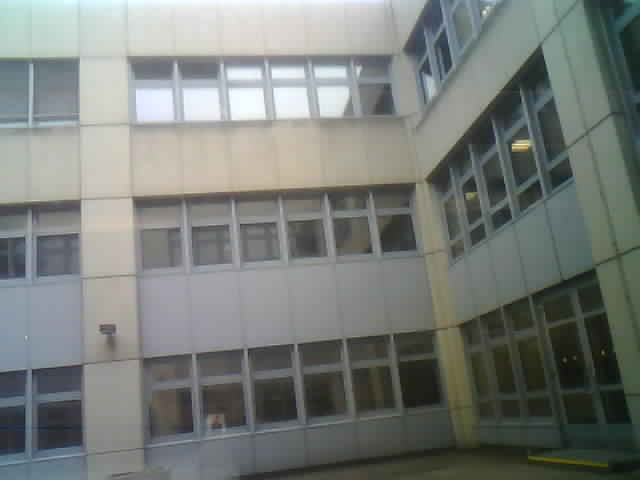
\includegraphics[width=0.7\textwidth, center]{img/cam_erstes_bild.png}
    \caption{Erstes empfangenes Bild der ESP32-CAM}
    \label{fig:cam_erstes_bild}
\end{figure}

\section{Core-Bibliothek}
\label{subec:robots_core}
Die Core-Bibliothek bildet eine weiter Abstrahierungsschicht zu den Funktionalitäten der Roboter-Hardware.
%
In unserem Modell stellt die Arduino-Bibliothek die erste Abstrahierungsschicht dar,
während die Code-Bibliothek diese weiter vereinfacht.
%
Durch diese Abstrahierung werden die Programme für die einzelnen Roboter um ein Vielfaches vereinfacht und dementsprechend übersichtlicher.
%
Wir können also die hier definierte Logik für jeden Roboter wiederverwenden,
anstatt drei mal fast genau das Gleiche zu programmieren.
%
Die Core-Bibliothek übernimmt alles von der WLAN-Verbindung,
über die Fernsteuerung per WebSockets,
bis hin zum Umschalten der einzelnen Pins zur Ansteuerung der Motortreiber.
%
Die Programmierung der einzelnen Roboter beschränkt sich also darauf,
die einzelnen Komponenten zu konfigurieren und miteinander zu verbinden.
%
Da Herr Gastgeber während der Projektwoche 2023/24 (Siehe Abschnitt \ref{sec:vorgeschichte}) bereits viel Zeit darin investiert hat,
die Bibliothek so modular und wiederverwendbar wie möglich zu gestalten,
konnten wir diese mit nur wenigen Modifikationen für unsere Diplomarbeit nutzen,
obwohl wir einen ganz anderen Hardwareaufbau verwenden.

\subsection{Module Allgemein}
\label{subsec:software_common_modules}
Wie schon erwähnt,
wurde die Core-Bibiliothek so modular wie nur möglich gestaltet,
um so viele Anwendungsfälle wie möglich abzudecken.
%
Jedes Modul implementiert eine der folgenden Klassen:
\begin{itemize}
    \item \texttt{Sensor}: Ein Sensor bzw. eine Sensorgruppe
    \item \texttt{Actor}: Ein Aktor bzw. eine Aktorgruppe
    \item \texttt{Interface}: Ein Interface zur Steuerung, z.B. WLAN
\end{itemize}
Theoretisch ist es damit möglich,
gemeinsame Funktionalität für alle Sensoren/Aktoren/Interfaces zu definieren,
wobei dies aber nicht tatsächlich realisiert wurde.
%
Jede dieser Klassen implementiert wiederum die Klasse \texttt{Module},
welche die folgenden Funktionen definiert:
\begin{itemize}
    \item \lstinline[language=c]|void init()|:
        Ähnlich wie \texttt{setup()} beim Arduino, nur im Kontext eines einzelnen Moduls.
        Wird verwendet um das Modul zu initialisieren.
    \item \lstinline[language=c]|void tick()|:
        Ähnlich wie \texttt{loop()} beim Arduino, nur im Kontext eines einzelnen Moduls.
        Sobald der Roboter alle Module fertig initialisiert hat,
        wird ständig durch ebendiese Module iteriert,
        wobei deren \texttt{tick()}-Funktionen aufgerufen werden. 
    \item \lstinline[language=c]|void terminate()|:
        Wird eigentlich nicht verwendet,
        da die meisten Module nicht zur mehrfachen Initialisierung gedacht sind.
        Im Sinne der Vollständigkeit gibt es trotzdem die Möglichkeit,
        diese Funktion zu implementieren.
\end{itemize}


\subsection{Robota}
Die Klasse \texttt{Robota}%
\footnote{Dieser Name wurde in der Anfangsphase des Projekts (Ende 2023) gewählt, 
        um Konflikte mit der veralteten ``Arduino Robot Library'',
        welche standardmäßig von der Arduino IDE inkludiert wird,
        zu vermeiden.
        %
        Seit dem Wechsel von der Arduino IDE auf PlatformIO stellt dieser potentielle Konflikt kein Problem mehr da}
ist für das Management der Module zuständig.
%
Hierzu gibt es drei Variablen, welche für die vollständige Funktion relevant sind:
\begin{itemize}
    \item \lstinline[language=c]|uint32_t ticks|:
        Eine globaler Zähler, welche einmal pro Tick ausgeführt wird.
        Dieser kann von Modulen verwendet werden, um bestimmte Tätigkeiten nur alle $n$ Ticks auszuführen.
        % TODO check if 100ns is realistic: ((2^32) - 1) / (t * (10^-9)) / (60 * 60 * 24 * 365.25)
        Bei einer durchschnittlichen Zeit von $t_{tick}=100ns$ pro Tick reichen 32 Bits aus,
        um die Roboter für etwas mehr als $t_{overflow}=1.36*10^{-9}$ Jahre zu betreiben,
        was für unsere Zwecke mehr als ausreichend sein sollte.
    \item \lstinline[language=c]|uint16_t moduleTypes[MAX_MODULE_AMOUNT]|:
        Hier wird Typeninformation zu den Modulen gespeichert.
        %
        Diese wird in den Funktionen \texttt{getModule} und \texttt{getFirstModule} verwendet,
        um die Module nach Typ zu filtern.
    \item \lstinline[language=c]|Module *modules[MAX_MODULE_AMOUNT]|:
        Dies ist die gesamte Liste an registrierten Modulen.
        %
        Mit \texttt{addModule} können Einträge hinzugefügt werden.
\end{itemize}
%TODO: Robota funktionen; insb. init() und tick()

\subsection{Sensoren}
\subsubsection{LD20 LiDAR}
Der Code zum Auslesen des LiDAR-Sensors basiert auf zwei Informationsquellen zum Protokoll:
%
Die offizielle Dokumentation von youyeetoo \cite{youyeetoo-ld20},
und einer Arduino-Bibliothek namens LD14P\_RP2040 \cite{ld20-library},
welche sehr stark modifiziert wurde, um Teil des \textit{Robota}-Frameworks zu werden.

Die Daten des LiDARs werden über eine RS-232-Schnittstelle (230400 baud 8N1) ausgelesen.
%
Hierbei werden nur von Seiten des LiDARs Daten gesendet,
es gibt keine Möglichkeit diesen über die UART zu steuern.
%
Jede Nachricht beginnt mit einem Header-Byte \texttt{0x54},
gefolgt von einem Info-Byte,
welcher die Art des Pakets angibt.
\begin{table}[H]
    \centering
    \begin{tabular}{r|l}
    Info-Byte & Pakettyp   \\ \hline
    0x2C      & Sensordaten \\
    0xE0      & Systemstatus \\
    0x0F      & Herstellerinfos   
    \end{tabular}
    \caption{Pakettypen des LD20}
    \label{tab:ld20-packet-overview}
\end{table}
Jedes Paket ist von einem Prüfbyte zur Fehlererkennung mittels CRC\footnote{Cyclic Redundancy Check} gefolgt.
%
Nur Pakete mit Sensordaten werden tatsächlich verarbeitet,
alle anderen werden verworfen,
da sie für diesen Anwendungszweck nicht unbedingt nötig sind.
%
Ein Paket mit Sensordaten besteht (neben den oben beschriebenem Header, Info-Byte und CRC)
aus der Geschwindigkeit des Messkopfes,
dem Startwinkel der Messung,
12 Messpunkten,
dem Endwinkel der Messung,
und einem Zeitstempel.
%
Die Messpunkte selber bestehen nur aus der gemessenen Entfernung und Intensität;
der Winkel muss selber berechnet werden.
%
Bei allen Einträgen die mehr als einen Byte beanspruchen wird der niederwertigste Byte zuerst übertragen,
des Protokoll ist also little-endian,
was bedeutet das die Rohdaten direkt in den Arbeitsspeicher von z.B. einem Arduino oder ESP32 übernommen werden können.
\begin{table}[H]
    \centering
    \begin{tabular}{l|l|l}
    Name            & Typ           & Einheit  \\ \hline
    Header          & fixed 0x54    &   \\
    VerLen          & fixed 0x2C    &   \\
    Geschwindigkeit & UInt16        & deg/s \\
    Startwinkel     & UInt16        & 0.01°  \\
    Messdaten       & 12x Messdaten &    \\
    EndWinkel       & UInt16        & 0.01° \\
    Zeitstempel     & UInt16        & ms \\
    CRC             & 1 Byte        &
    \end{tabular}
    \caption{Paketformat des Messdatenpakets}
    \label{tab:ld20-measurement-packet}
\end{table}
\begin{table}[H]
    \centering
    \begin{tabular}{l|l|l}
    Name        & Typ       & Einheit   \\ \hline
    Distance    & UInt16    & mm        \\
    Intensity   & Uint8     &           \\ % Einheitslos
    \end{tabular}
    \caption{Format der rohen Messdaten}
    \label{tab:ld20-measurement-data}
\end{table}
Der Winkel einer einzelnen Messung kann mittels linearer Interpolation wie folgt berechnet werden:
\begin{equation}
    \alpha = \alpha_{s} + \frac{\alpha_{e}-\alpha_{s}}{n-1}*i = \alpha_{s} + \frac{\alpha_{e}-\alpha_{s}}{11}*i
\end{equation}
Hierbei ist $\alpha$ der Winkel einer einzelnen Messung,
während $\alpha_{s}$ und $\alpha_{e}$ respektive den Start- und Endwinkel der Messserie repräsentieren.
$n$ steht für die Anzahl an Messungen pro Messserie und ist bei uns konstant $12$,
weshalb $n-1$ auf $11$ vereinfacht werden kann. $i$ ist der nullbasierte Index der einzelnen Messung im Kontext der Messserie.

%\begin{tikzpicture}[node distance = 3cm]
%    \node [terminator, fill=blue!20] (start) {\textbf{Komplettes Packet empfangen}};
%    \node [process, below of=start] (crcCalc) {CRC berechnen};
%    \node [data, fill=blue!20, below of=crcCalc] (data) {Provide data};
%    \node [decision, fill=blue!20, below of=data] (crcCheck) {Daten gültig?};
%    \node [process, fill=red!20, right of=crcCheck, node distance=5cm] (error) {Paket verwerfen};
%    \node [process, fill=green!20, below of=crcCheck] (success) {Success};
%    \node [terminator, fill=blue!20, below of=success] (end) {\textbf{End}};
%    \path [connector] (start) -- (data);
%    \path [connector] (data) -- (crcCheck);
%    \path [connector] (crcCheck) -- node[anchor=south] {Nein} (error);
%    \path [connector] (crcCheck) -- node[anchor=east] {Ja} (success);
%    \path [connector] (error) |- (end);
%    \path [connector] (success) -- (end);
%\end{tikzpicture}


\subsubsection{Drehgeber}
Die beiden Drehgeber,
welche jeweils an einen der Motoren montiert sind,
werden von dem Modul \texttt{RotaryEncoder} ausgelesen.
%
Dieses Modul hat eine beim Kompilieren festgelegte Anzahl an sogenannten ``Ausgabe-Kanälen'',
da die Daten der Drehgeber an mehreren separaten Stellen verarbeitet werden müssen.
%
Die verwendete Zahl an Kanälen wurde auf Vier festgelegt, kann in der Zukunft aber sehr einfach geändert werden.
%
Anstatt die aktuelle Geschwindigkeit zu berechnen,
werden jeweils für jeden Kanal der Zeitpunkt des letzten Auslesens
und die Zahl an Impulsen vom Drehgeber seit ebendiesem Zeitpunkt gespeichert.
%
Dadurch können Module, welche die Daten verarbeiten,
selber wählen, über welchen Zeitraum die Geschwindigkeit berechnet wird.
%
Das ist ein netter Nebeneffekt, aber eigentlich wurde dieser Ansatz gewählt,
weil das Datenformat zur Übertragung an den Server Daten in ebendiesem Format erwartet.
%
Da das Zählen selber durch Interrupts gelöst wurde
und ISRs\footnote{Interrupt Service Routines}
nicht Mitglieder einer instanziierten Klasse sein dürfen (bzw. können),
muss zur Verwendung des \texttt{RotaryEncoder}-Moduls eine globale Funktion erstellt werden,
welche als ISR dient.
% TODO: function identifiers?
Diese Funktion soll einzig und allein \texttt{RotaryEncoder\#pulse()} aufrufen
und mittels \texttt{RotaryEncoder\#attachISR()} mit dem Trigger-Pin des Drehgebers ``verbunden'' werden.
%
\texttt{RotaryEncoder\#pulse()} regelt die Erhöhung der Zähler für alle Kanäle.
%
Beim Auslesen eines Kanals werden sowohl der Zeitstempel als auch der Zähler automatisch zurückgesetzt.

\subsubsection{MPU6050}
Da für das Auslesen der Rohdaten des eingebautem Gyroskop/Accelerometer
\texttt{MPU6050} einer externe Bibliothek \cite{adafruit-mpu6050} verwendet wurde,
war der Aufwand hierfür eher gering.
%
Das \texttt{MPU6050}-Modul sorgt also lediglich dafür,
dass die Werte nicht mehrmals pro Tick schnell hintereinander ausgelesen werden.
%
Erreicht wird das, indem ausgelesene Werte zwischengespeichert werden,
bis der aktuelle Tick vorbei ist.
%
Werden die Werte also mehrmals pro Tick abgefragt,
wird einfach der zuletzt ausgelesene Wert zurückgegeben.

\subsection{Aktoren}
\subsubsection{GenericDigitalOutput}
Das Modul \texttt{GenericDigitalOutput} dient als Grundlage zur Verwendung von anderen Modulen,
um einen digitalen Ausgang anzusteuern.

\subsubsection{PwmOutput}
Das Modul \texttt{PWMOutput} dient als Grundlage zur Verwendung von anderen Modulen,
um einen PWM-Ausgang anzusteuern.
%
Hierzu wird anstatt den standardmäßigen Arduino-Funktionen
direkt die ESP32 \texttt{ledc}-API verwendet,
um bestmögliche Konfigurationsoptionen zu erreichen\cite{esp32-ledc}. %TODO not sure if this sounds good
%
Weiters gibt es sowohl die Möglichkeit den Duty-Cycle direkt einzustellen,
oder anhand der erwünschten Breite des Impulses (in Mikrosekunden) zu berechnen;
dies ist insbesondere zum Einstellen vom Servomotoren nützlich.
%
Das Modul wählt automatisch den bestmöglichen PWM-Kanal:
%
Da beim ESP32 sich jeweils zwei PWM-Kanäle einen Timer teilen,
müssen diese die gleiche Frequenz haben.
%
Beim Initialisieren des PWM-Moduls wird automatisch nach einem Timer mit gleicher Frequenz gesucht,
welcher noch Platz für einen weiteren PWM-Kanal hat.
%
Wurde kein solcher Timer gefunden,
wird ein anderer konfiguriert.
%
Zu guter Letzt sorgt das PWM-Modul automatisch dafür,
dass die höchstmögliche Auflösung verwendet wird.
%
Die PWM-Kanäle des ESP32 haben eine zur Frequenz indirekt proportionale Auflösung \cite{esp32-technical-reference}.
Die maximale Signalfrequenz $f_{out}$ bei gegebener Auflösung $R$ lässt sich wie folgt berechnen:
\begin{equation}
    f = \frac{f_{clk}}{N*2^{R}}
\end{equation}
Daraus ergibt sich zur Berechnung der maximalen Auflösung bei gegebener Signalfrequenz:
\begin{equation}
    R = \log_2\left( \frac{f_{clk}}{f_{out}*N} \right)
\end{equation}
Hierbei ist $f_{clk}$ das gegebene Taktsignal des Timers und $N$ der Wert des Prescalers.
%
$R_{max}$ wird abgerundet.

Zur Berechnung der höchstmöglichen Auflösung $R_{max}$ wird $N=1$ gesetzt und das Ergebnis abgerundet.
%
Zu Beachten ist hierbei, das alle Ergebnisse,
welche größer als 20 sind,
als 20 anzunehmen sind.
% ^ TODO komische docs
%
Tatsächlich gibt es auch eine minimale Auflösung,
wobei es ja immer möglich ist,
die Auflösung eines Signals künstlich zu verringern.
%
Die minimale Auflösung kann berechnet werden, indem $N=1023+\frac{255}{256}$ gesetzt wird.
Das Ergebnis wird aufgerundet und hat einen Minimalwert von 1.

Bei Verwendung der \texttt{APB\_CLK}, mit 80MHz als Taktsignal,
ergeben sich also folgende Werte:
\begin{table}[H]
    \centering
    \begin{tabular}{r|l|l}
    $f_{sig}$ [Hz]  & $R_{max}$ [bits] & $R_{min}$ [bits] \\ \hline
    1k        & 16 & 7 \\
    2k        & 15 & 6 \\
    5k        & 13 & 4 \\
    10k       & 12 & 3 \\
    20k       & 11 & 2 \\
    50k       & 10 & 1 \\
    100k      & 9  & 1 \\
    1M        & 6  & 1 \\
    2M        & 5  & 1 \\
    5M        & 4  & 1 \\
    \end{tabular}
    \caption{PWM-Auflösungen bei gewählten Frequenzen}
    \label{tab:pwm-resolution}
\end{table}

\subsubsection{SingleMotorOutput}
Das Modul \texttt{SingleMotorOutput} verwendet die bereits beschriebenen Module
\texttt{GenericDigitalOutput} und \texttt{PWMOutput},
um einen einzelnen Motor mittels eines Motortreibers anzusteuern.
Um die Verwendung mit möglichst vielen unterschiedlichen Motortreibern zu gewährleisten,
gibt es drei unterschiedliche Möglichkeiten, die \texttt{GenericDigitalOutput}s zu konfigurieren:
\begin{itemize}
    \item Verwendung eines Pins für \texttt{forward}
    \item Verwendung eines Pins für \texttt{backward}
    \item Verwendung beider Pins
\end{itemize}
In Kombination mit dem Tumbller wurde die erste der drei Möglichkeiten gewählt.
%
Der eingebaute Motortreiber erwartet zwar sowohl ein \texttt{forward}- als auch ein \texttt{backward}-Signal,
jedoch wird das \texttt{backward}-Signal hardwaremäßig durch Inversion von \texttt{forward} generiert.
%
Die Richtung und Geschwindigkeit werden als signierte 16-Bit Integer gegeben,
wobei negative Werte als Rückwärtsfahren interpretiert werden.
%
Es bleiben also 15 Bits Genauigkeit für die Geschwindigkeit,
was mehr als ausreichend ist.
%
Das \texttt{SingleMotorOutput}-Modul stellt lediglich eine Steuerung dar,
die Regelung der Motorgeschwindigkeit mit Rückkopplung durch Drehgeber wird andernorts realisiert.

\subsubsection{BalanceController}
Die Gesamtheit der Aktoren kommt im \texttt{BalanceController} zusammen:
Hier werden die Daten vom \texttt{MPU6050} ausgelesen,
zur Verbesserung der Genauigkeit durch den \texttt{KalmanFilter} gefiltert,
und als Rückkopplung in einen PID-Regler eingegeben,
welcher mittels zwei \texttt{SingleMotorOutput}s die beiden Motoren kontrolliert.
%
Als Führungsgröße wird hier zusätzlich die gewollte Geschwindigkeit und Auslenkung eingegeben,
welche vom Server an die Roboter gesendet wird.

TODO mehr Beschreibung 

\subsection{Interfaces}
TODO

\subsection{Hilfsklassen}
Der Robota-Framework stellt zwei Hilfsklassen (engl. ``Utilities''/``Utils'') zur Verfügung:
\texttt{KalmanFilter} und \texttt{PIDController}.

\subsubsection{KalmanFilter}
Kalman-Filter werden allgemein zu Schätzung von Systemzuständen verwendet,
welche nur ungenau gemessen werden können.
%
Die konkrete Anwendung in diesem Projekt beschränkt sich auf die Berechnung
der Neigung der Roboter basierend auf den relativ ungenauen Messdaten des MPU6050.
%
Hierbei werden die Daten des Gyroskops mit denen des Accelerometers kombiniert,
um eine möglichst genaue Schätzung des Neigungswinkel zu erreichen\cite{digikey-kalman}.
%
Diese sogenannte Sensorfusion ermöglicht es,
die Messfehler der beiden Sensoren auszugleichen,
um einen genauen Wert zu erreichen.
%
Der verwendete Code zum Kalman-Filter basiert auf einem modifiziertem Beispielcode von Kristian Lauszus \cite{lauszus}.
% TODO maths?

\subsubsection{PIDController}
PID-Regler (Proportional, Integral, Differential) werden verwendet,
um eine Regelstrecke bestmöglich zu regeln.
%
Im Kontext der Tumbller werden PID-Regler an zwei Stellen eingesetzt:
\begin{itemize}
    \item Regelung der Motorgeschwindigkeit
    \item Regelung der Neigung und Auslenkung der Roboter
\end{itemize}
% TODO more elaborate description; maths?

\section{Guide}
\label{subsec:software_guide}
Die Software von \textit{Guide} ist in diesem Projekt in dem Sinne einzigartig,
dass,
zusätzlich zur Steuerung des Roboters selber,
die gemessen LiDAR-Werte empfangen,
aufbereitet,
und mit möglichst wenig Verzögerung an den Server weitergeleitet werden müssen.
%
Der Erfolg des ganzen Projekts ist also von der Verlässlichkeit dieser Software abhängig.
%
Abgesehen davon verhält sich der Guide eigentlich genau gleich wie Tamerlan und Bambi:
%
Befehle werden vom Server empfangen und ausgeführt,
Messwerte werden an den Server weitergeleitet.
%
Da auch die Aufbereitung der LiDAR-Daten bereits in der Core-Bibliothek realisiert wurde,
ist die Software für den Guide ebenso wie bei den anderen Robotern größtenteils Plug\&Play.

\section{Tamerlan}
\label{subsec:software_tamerlan}

\section{Bambi}
\label{subsec:software_bambi}

	% Software Backend (Python)
% Zuständig: Jones

% wie/wo soll protobuf erklärt/erwähnt werden?

\chapter{Software - Backend}
\label{sec:software_backend}
\initials{JS}
Das Backend ist die Zentrale Rechenstelle, 
welches in mehrere Komponenten aufgeteilt ist.
% generell zum backend

\begin{figure}[H]
    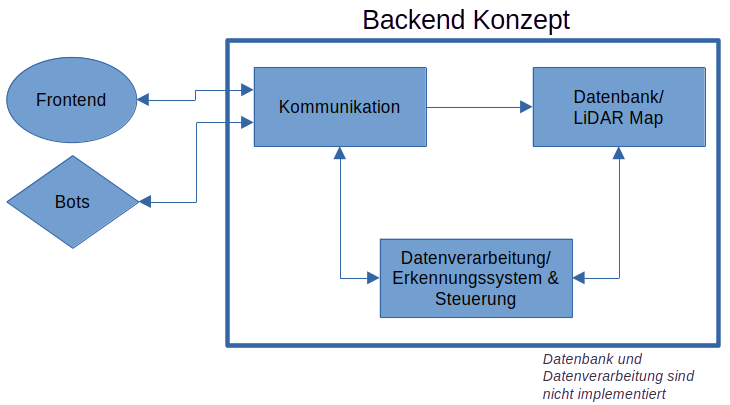
\includegraphics[width=\textwidth, center]{img/backend-konzept.png}
    \caption{Backend Konzept}
    \label{fig:backend_konzept}
\end{figure}
% grafik anpassen

Wodurch es verantwortlich für die Kommunikation und Datenerfassung 
zwischen allen Teilnehmer. 
Dazu gehören die drei Roboter, welche uns die Daten liefern 
wie LiDAR, Beschleunigungssensor etc., 
und das Frontend zu dem die Daten zur Visualisierung und Mitverfolgung gesendet werden
und gegebenenfalls auch Befehle empfingt.
\\
Weiters findet hier die Zentrale Datenverarbeitung und Verwaltung statt, 
dies ist verantwortlich für die Erstellung der LiDAR Map, 
der Ermittlung der Roboter Positionen 
und gegeben falls Berechnung der Messwerte. 
% im falle ineffizient etc
\\
Und Steuerung der Roboter mithilfe eines Erkennungssystems 
welches bestimmte Kennzeichen in den erhaltenen Daten Ausschau hält und 
darauf Kennzeichen für die einzelnen Bots erkennt und verfolgt, 
um entsprechend die Positionen aller Bots relativ zur LiDAR Map ausfindig zu machen.
% 
% Die Zentrale Datenverarbeitung und autonome Steuerung der Roboter sind 
% im zu zeitigen Prototypen stand nicht implementiert.
% % stattdessen weiterleitung und fernsteuerung
% TODO 
\\
Und letztendlich die Datenbank welches die etwaigen Daten speichert 
von der Datenverarbeitung und Erkennungssystems, 
dazu gehört insbesondere die LiDAR map.

Für das Backend wurde Python gewählt, 
welches von seiner Vielzahl von Standardpaketen und 
großen Anzahl an externen Paketen und Frameworks, 
eine effiziente und schnelle Programmierung ermöglicht, 
auch unterstützt durch eine aktive Community.
% 
Für dieses Projekt wurde es gewählt aufgrund seiner Vielseitigkeit, 
speziell in Bezug auf den unterschiedlichen Task die ausgeführt werden müssen, 
hauptsächlich der Kommunikation und Datenverarbeitung 
Felder in die Python üblicherweise verwendet werden.
% 
Darauf müssen auch mehrere Verbindungen offen bleiben und verwaltet werden,
und dies schnell zu realisieren mithilfe von Paketen 
die uns ermöglichen aufs wesentliche zu fokussieren.
% 
Eine schnelle Programmierung und Modifizierung, 
weil das Backend voraussichtlich mit dem zum zeitigen Projektstand wächst, 
ganz wichtig für die Datenverarbeitung und Steuerung 
da diese sich im Laufe des Projekts stark ändern kann,
aufgrund dessen, dass die Methoden und Systeme nicht endgültig feststehen, 
und teilweise noch definiert werden müssen.
% 
Und letzteres auch wegen Erfahrungen mit dem Vorgänger Projekt, 
denn ein wesentlicher Teil davon bestand auf die Kommunikation über Websockets.
% Gelaber über python
% wegen math Funktionen...
% schnelle Modifizierung 
% packet/ Bibliothek Fokussierung auf Einfachheit
\section{Systembeschreibung}
\initials{JS}
% drunter verschoben weil besseres layout?
In disem Abschnitt wird genauer 
über die geplanten einzelnen Komponenten gesprochen 
und deren Funktion.

Zu beachten ist, dass nicht alle geplanten Systeme, die hier Beschrieben sind,
implementiert wurden und manche noch in der Konzeptphase sind.
Für den tatsächlichen Stand siehe Abschnitt \ref{subsec:backend_aktueller_stand}.

\subsection{Datenverwaltung}
\label{subsec:backend_data}
\initials{JS}
% übersicht über die drei komponenten und wie ungefähr der datenfluss aussieht?
TODO
% Datenbank für lidar?
TODO

Dieser Abschnitt bespricht kurz den Datenablauf 
zwischen den Teilnehmer und den internen Komponenten.
% 
Weil die Datenverarbeitung noch nicht realisiert ist 
kann noch nicht viel weiter zur Verwaltung gesprochen werden.

Das Frontend und die Roboter kommunizieren hauptsächlich 
über Websockets mit den Protobufs.

\subsection{Kommunikation}
\label{subsec:Kommunikation}
\initials{JS}
Die drei Roboter sind aktive Teilnehmer in der Kommunikation, 
das heißt es ist zu erwarten, dass die Verbindung konstant aufrechtzuerhalten ist,
bidirektional und dies auch in einem zeitlichen verhalten geschieht. 
Insofern muss weiter sichergestellt werden das ein konstanter Kommunikationsfluss 
ermöglicht bleibt.

Zur Verbindung entschieden wir uns für das Kommunikations-Protokoll Websocket, 
diese ermöglicht eine bidirektionale, 
persistente Verbindung zwischen einem Client und einem Server,
welches im Vergleich zu gewöhnlichen HTTP-Anfragen offen bleibt, 
wodurch Echtzeitkommunikation möglich ist.
% könnte man mehr ausschreiben aber schau ma später

\subsection{Datenverarbeitung}
\initials{JS}
% TODO
Ein Teil des Servers ist die Verarbeitung der erhaltenen Daten, 
die entweder zum Frontend weitergeleitet wird, oder vom Server verarbeitet.
% 
Um große Belastung mit Sensordaten Berechnung auf den Roboter zu vermeiden,
werden einige Arbeiten auch auf den Server entlasten.
Ein weiterer Grund dafür ist, aufgrund dessen das mit Python 
bereits ausgebaute Mathematik Pakete zur Verfügung stehen
und die Sensordaten zu Bearbeiten.
Und auch ausgebautes Daten Analyse und Manipulation Pakete.


\subsection{Erkennungssystem}
\initials{JS}
Geplant war das die erhaltenen Daten über das Datenverarbeitungssystem 
über die Zeit hinaus eine Karte erstellt sozusagen die LiDAR map,
welche in einer Datenbank abgespeichert werden.
% 
Über die Zeit werden Datenpunkte gesammelt, 
die sich mehr nach einem gewissen Muster sammeln 
und ein klareres Bild über die Form eines Raumes geben.
Diese Muster, wie gerade Linien und Ecken werden vom System erkannt
und mit diesen Eigenschaften auch ermittelt, 
wo ungefähr sich der Guide im Raum befindet.
% 
Dies wird mit einem weiteren Erkennungssystem für Tamerlan \& Bambi,
welches zuständig ist die position der zwei zu ermitteln.
Indem die Bots identifizierbare reflektieren Objekte befestigt kriegen,
Beispielweise mehrere Zylinder wodurch sie erkannt werden können.
%
Mit diesen Informationen kann die Steuerung der Roboter folgen.
% füge skizzen hier oder erklär anderen Kapitel?
% Kugel, stab, mehrere stäbe, reflektierendes material

Eine genauere Beschreibung der LiDAR Karte und wie diese aussieht
ist im Frontend Abschnitt \ref{subsec:frontend_lidar_map} 
auf Seite \pageref{subsec:frontend_lidar_map} zu finden.

\subsection{Steuerung der Roboter}
\label{subsec:backend_robot_detection}
\initials{JS}
% TODO
Zurzeit nicht realisiert.
% spätester schritt weil funktionierende Strategie benötigt wird zur Erkennung
% Datenbank/ Datenbearbeitung

Die Aufträge der einzelnen Bots sind in den Entsprechenden Kapitel genauer beschrieben.
% schau was da steht und was speziell hier klargemacht werden muss

Es sind zwei Steuerungen geplannt die manuelle Steuerung 
und die Automatisierte.
% 
Die manuelle Steuerung geschieht über das Frontend 
womit man die Roboter mit hilfe der Visualisierungen 
und oder Video Übertragung steuern kann.
% 
Die Automatisierte Steuerung geschieht mithilfe das Erkennungsystem 
und soll die Bots erlauben die erstellte LiDAR Karte zu navigieren
und erlauben die zwei Blinden Bots Tamerlan \& Bambi den Guide zu folgen.
% verwendung von code vom vorgänger Projekt

\section{Aktueller Stand}
\label{subsec:backend_aktueller_stand}
\initials{JS}
% Womöglich Teile zu Ergebnisse verschieben?
Zum Zeitpunkt dieser Diplomarbeit Abgabe 
sind nicht alle geplanten Features für das Backend zeitlich zusammengekommen.
Wodurch der Großteil der Backendserver Seite nicht realisiert werden konnte.

Zur Überbrückung wurde der Kommunikationsteil so realisiert, 
dass es als Weitergabe fungieren soll.
Dies wurde so realisiert, indem die Daten 
zwischen einem Bot und dem Server weitergegeben werden, essenziell ein Router. 
Der nächste Schritt besteht dann über eine Prototyp Steuerung 
Befehle zu den einzelnen Bots zu senden.

Die Prototyp Steuerung ist realisiert als eine manuelle Steuerung, 
wo dem gewählten Roboter manuell von einem Bediener bedient.
In Zukunft kann die manuelle Steuerung als eine weitere Option beibehalten werden, 
die die automatisierte Steuerung überschreiben kann. 
Dies kann verwendet werden, 
um Beispielweise den Guide manuell in bestimmte Bereiche zu führen.
Anderes falls auch für Test und Debug Zwecke, 
sowie manuell eine neue Datenerfassung zu erzwingen.

\section{Backend - Code}
\initials{JS}
In diesem Abschnitt wird genauer zum Code des Backend Prototyps eingegangen 
und dessen technischen Realisierung. 
Was genau die einzelnen Teile des Backends zu erledigen haben, 
wie diese Probleme bewältigt und realisiert wurden.
Weiters werden auch beschrieben welche Pakete und Werkzeuge verwendet wurden. 

\subsection{Zusätzlich verwendete Tools und Workflow}
\initials{JS}
% algemein zu python workflow
% womöglich unötig
% TODO
\subsubsection{Formatter und Linter} 
\initials{JS}
Um gute Lesbarkeit zu gewährleisten 
ist eine ordentliche Struktur und Format in jedem Code zu erwarten, 
jedoch ist es schwierig eine gute konsistent beizubehalten, 
weshalb Formatierungstool und Linters häufig Verwendung finden. 
% 
Linters sind Tools welche automatisch den code überprüfen, um auf Fehler zu prüfen, 
stilistische Fehler und Einhaltung von Codierung Standards festzustellen.
Diese soll helfen die code Qualität zu verbessern 
und womögliche Fehler vorzeitig zu erkennen.

Die Standard Erweiterung für Python von Visual Studio Code 
beinhaltet keinen Standard Formatierungstool.
Dafür wurde der Formatter \texttt{autopep8} verwendet, 
weil er die Eigenschaft hat den original still des Schreibers beibehalten
und nur hauptsächlich Änderungen für die Lesbarkeit durchzuführen. 
Dazu passend ist der Linter \texttt{Flake8} welcher standardmäßig 
den gleichen Styleguide \text{PEP 8} folgt.
% weil vscode es standart mäßig Formatierung nicht mitliefert
\subsubsection{venv/environment management}
\initials{JS}
% TODO


\subsection{Python Packages}
\initials{JS}
% TODO schau dir dieses abschniit nochmal durch
Um gegebene Funktionen zu Gewehrleisten sind weitere externe Paketen nötig, 
die nicht teil der Standard Paketen sind.
Welche zu diesem Stand verwendet wurden, ist in diesem Abschnitt erklärt.

\subsubsection{websockets}
\initials{JS}
Für Python ist ein Websocket Paket namens 'websockets' vorhanden 
welches die Client-Server Kommunikation um ein Vielfaches vereinfacht 
da man sich keine Sorge über Handshakes, Ping Pongs, 
oder anderes verhalten der Websocket Spezifikation, 
da es alles von dem Paket behandelt wird 
und man sich mehr auf die Applikation fokussieren kann. 
Es sind dennoch einige Parameter zum zur Verfügung gestellt zur Modifizierung, 
falls benötigt.
% code beispiele?

% erklärung zu den packet Webscoket
Websockets Standard Implementierung basiert auf asyncio.
%  
Asyncio ist die eingebaute Implementierung von Koroutinen in Python,
dies erlaubt das Schreiben von asynchronen Frameworks, 
öfters verwendet für I/O limitierte Netzwerk Codes.
% snippet zu asyncio, könnte mehr schreiben?
Alternative ist eine threading Implementierung verfügbar für Websockets, 
die üblichere Implementierung von mehreren Tasks, 
jedoch würde für den zum zeitigen Prototyp Entwicklung-Stand dagegen entschieden,
aufgrund der möglichen erweiterten Komplexität von Thread sicheren code Ausführung.
% warum nicht? kann später bei optimierungsmöglichkeiten erklärt werden
Eine Sans-I/O Implementierung ist auch vorhanden 
jedoch für dieses Projekt zurzeit irrelevant.

\subsubsection{protobuf}
\initials{JS}
Das Besondere an der protobuf Implementierung hier in Python ist,
das sehr viel von der protobuf Paket selbst erledigt wird.
Im Vergleich zum Vorgänger Projekt wo die Datenpakete manuell hergerichtet werden
und zum richtigen Byte Format konvertiert, wird mit Protobuf ein Objekt erstellt 
und jeweils die gegebenen Variablen angesprochen, 
diese mit einem einzelnen Befehl ins sende Format formatiert und genauso zurück
und von den gegebenen Tasks weiterverarbeitet werden kann.
% verhalten in python
% wie anders

% Kurzeitig gab es das Problem wie genau mit dem Python protobuf paket zu arbeiten ist,
% aufgrund dessen das die dokumentation nicht der von anderen Python Paketen gleicht
% und alle Informationen hauptsächlich von der Anleitungen zu Wünschen übrig lässt.
% Ich hatte einfach ein wenig probleme es anfänglich zu kapieren aber ging schnell

\subsection{Prototyp Kommunikation - test\_server\_passby.py}
\initials{JS}
In diesem Abschnitt wird über den zu zeitigen Prototyp Kommunikation 
und bestimmten technischen Implementierungen angesprochen.

Der Prototyp hat die Funktion zwei Typen von Verbindungen zu bearbeiten.
% 
Einer seit die Bots welche als Server agieren, 
dies Bedeuten, dass dieser Backend Server muss sich mit den drei Robotern verbinden.
Während das Frontend standardmäßig als Client fungiert, 
dies Bedeutet, dass die Clients eine Verbindung mit dem Backend Server herstellen.
% 
Anderer seits die Verbindung mit den Frontend 
welcher vom Server für einkommende Verbindungen bereitgestellt werden müssen.
% 
Die Daten die von der jeweiligen Seite ankommt, 
wird zurzeit zur gegenseitigen Stelle weitergeleitet.

Dementsprechend ist die Kommunikation auf zwei Tasks aufgeteilt,
die des Frontends und die der Roboter.
Beide Tasks starten ein weiteren Subtask, welcher nebenbei laufen wird, 
dieser hat entsprechend die Aufgabe so lange die Websocket Verbindung offen ist,
die ankommende Pakete erwartet und diese entsprechend in eine Queue Puffer ablegt, 
um weiter verarbeitet zu werden. 

Beide Task verarbeiten die Queues, 
in dem eine bestimmte Anzahl der Elemente im Puffer 
einzeln geholt und die Protobuf Wrapper verarbeitet zu werden.
% 
Im zum zeitigen Prototyp werden die Daten in die Konsole ausgegeben,
und zur Sendung der Gegenseite in eine weitere Queue 
für einen beliebigen Roboter bereitgestellt, 
oder im Fall beim zum zeitigen Roboter Händler an alle verbundenen Frontends gesendet.
% 
Dies symbolisiert in den nächsten Iterationen die Weitergabe 
in die Datenbank und Datenverarbeitung.

% übersichtsgrafik über teilnehmer und wie datenablauf funktioniert
% asyncio - warum
% main task überblick (server und drei clients) warum so aufgeteilt?
% subtask

\subsubsection{asyncio}
\initials{JS}
% erklärung zu asyncio
Um mehrere separate Task auszuführen wurde Asyncio,
die eingebaute Implementierung von Koroutinen in Python verwendet.
% 
Asyncio funktioniert, indem Tasks sich den Event Loop nehmen und mit dem 'await' 
Befehl anderen Tasks erlaubt sich den Event Loop zu nehmen, 
im Vergleich zu üblichen Multitasking
wo jeder Task eine feste Zeit zugeschrieben bekommt vom Betriebssystem.

TODO

\subsubsection{Queue Buffers}
\initials{JS}
% FIFO Queues
% Wichtigkeit nicht blockierendes verhalten um asynchrones workflow zu gewährleisten
Damit die Prozesse im Backend nicht gezwungen sind immer zu bearbeiten, 
wenn und falls Einkommen Nachrichten zu bearbeiten sind, 
wird der Empfang von Websockets abgekoppelt von der backend Logik.
Dafür wurden Queues, realisiert als FIFO, verwendet, also ein zwischen speicher 
wo die erhaltenen Daten von den Websockets landen, 
um dann entsprechen weiter zu bearbeiten.
% 
Somit können wir einen Prozess starten, welches auf eingehende Nachrichten warten kann,
während unser Backend andere Prozesse ausführt.
% kann mehr dazu schreiben
% ermöglicht auch sachen etc.
% TODO

\subsection{Prototyp manuelle Steuerung}
\initials{JS}
Die Prototyp Steuerung soll ein Bediener erlauben manuell den Bot zu Steuern,
indem wir mit einer Eingabe bewegen können. 
% 
Dafür verwenden wir ein Controller 
aufgrund dessen das wir bereits im Vorgänger Projekt,
eine Form solcher Steuerung realisiert haben. 
Deshalb ist ein Großteil der Arbeit hier die Anpassung auf dem neuen Datenformat, 
Verwendung neuer Websocket Pakete und Modifizierung der Berechnungen.
% 
Anfänglich ist geplant es, als einzelnen Skript zu realisieren, 
welcher den Platz des Frontends nimmt, 
und im Laufe des Projekts ins Frontend integriert oder neu implementiert wird.

% TODO aktualisiere dies entsprechend
Zum Zeitpunkt des Schreibens diesen Abschnitt der Diplomarbeit 
ist dies mitten in der Bearbeitung.
% TODO
\subsubsection{Vorgänger Code}
\initials{JS}
Erklärung was der alte Code alles macht.
\subsubsection{Anpassung}
\initials{JS}
Wie es angepasst wurde.

\subsection{Konsolen Ausgabe}
\initials{JS}
% siehe print_wrapper_content.py
Der Skript \texttt{print\_wrapper\_content.py} hat die simple Funktion 
die Daten von einem Protobuf Wrapper in die Konsole auszugeben, 
in eine einfache Menschlich lesbare Struktur. 
Hauptsächlich genutzt für Debug und Entwicklungsschritte.

\begin{figure}[H]
    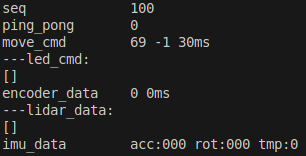
\includegraphics[width=0.5\textwidth, center]{img/Backend/print_wrapper_all.png}
    \caption{Python - Protobuf Konsolen Ausgabe}
    \label{fig:py_konsole_o}
\end{figure}

In Zukunft kann dies durch die Datenbank oder ein CSV log abgelöst werden 
und somit auch bessere Systeme implementiert werden.
% 
Diese könnten automatisch für sonderbare Änderungen suchen 
und entsprechen Melden und in einem Log abspeichern.

\subsection{Optimierungsmöglichkeiten}
\initials{JS}
\label{subsec:Optimierungsmöglichkeiten}
\subsubsection{uvloop - schnellere Koroutinen}
\initials{JS}
% uvloop - drop in replacement
% https://github.com/MagicStack/uvloop
uvloop ist ein schneller drop-in Ersetzung von der eingebauten asyncio Event Loop, 
dieser ist entsprechend in Cython entwickelt 
(Cython ist entsprechend Python aber als Performanten C code compiliert).
Ziel dieser Ersetzung ist es asyncio um einiges schneller zu machen 
aber nicht von der Referenz verhalten von asyncio abzuweichen. 
Als drop-in Ersetzung geht dies so weit, 
dass die Abweichungen als Fehler kategorisiert werden.
% 
Während der Prototyp Phase dieses Projekts 
ist man auf der Standard Implementierung geblieben, aufgrund Stabilität
und weil uvloop bis später im Projekt unbekannt geblieben ist.
In Zukunft wird jedoch eine Implementierung in Betracht gezogen,
aufgrund der vorhin genannten Eigenschaften.
% 
Insbesondere wenn die nachfolgenden Projekte weiter skalieren.

% compelierung python code
\subsubsection{Kompilierung}
\initials{JS}
Es ist möglich Python code genau so wie jedes andere Programm zu kompilieren,
jedoch ist dies standardmäßig nicht nötig 
da der Interpreter Cpython automatisch Python byte code kompeliert (in PYC Dateien).
Das prekompilieren wird hauptsächlich dafür verwendet um die Start zeit zu verringern 
und um den Code für die gewählte Platform einfacher zu verteilen,
weil man keine weiteren Pakete installieren muss sondern
nur die PYC Datei allein genügt.
% Dies ist jedoch für dieses Projekt irrelevant.

\subsection{threading vs asyncio}
\initials{JS}
% TODO threading warum nicht streng nötig 
% (hauptsächlich limitiert über Wifi I/O nicht anzahl an geräten & )
% falls anzahl größer wird dann villeicht

\section{Probleme}
\initials{JS}
\subsection{Linux Modifikationen}
\initials{JS}
Es kam das Problem auf, dass die lokale IP suche auf Linux Ubuntu nicht funktionierte.
Dies lag daran, dass die vorherige Variante, 
welcher mithilfe der Domain Name auf die lokale IP-Adresse findig wurde.
Jedoch wurde auf Linux eine andere Adresse zurückgeliefert, 
zwar die Loopback-Adresse \texttt{127.0.1.1}. 
Diese Adresse wird verwendet, um den \texttt{host\_name} eine Adresse zuzuweisen,
im Falle das kein Netzwerk vorhanden ist. 
Sonst kann eine permanente IP-Adresse hier zugewiesen werden.
% https://askubuntu.com/questions/754213
% /what-is-difference-between-localhost-address-127-0-0-1-and-127-0-1-1

Als Lösung öffnet das Programm temporär ein Socket 
und findet mit dieser die lokale IP-Adresse, und dadurch Plattform unabhängig.
\begin{lstlisting}[language=python, gobble=4]
    import socket

    def get_local_ip():
    """
    opens a temporary socket connection and retrieves the local IP
    """
    s = socket.socket(socket.AF_INET, socket.SOCK_DGRAM)
    try:
        # doesn't even have to be reachable
        s.connect(('10.255.255.255', 1))
        IP = str(s.getsockname()[0])
    except Exception as b:
        print("error at figuring out local ip")
        print(b)
        exit
    finally:
        s.close()
    return IP
\end{lstlisting}

\subsection{Potenzielles blockierendes verhalten}
\initials{JS}
% bot_handler und server nicht separat gestartet werden.
Obwohl die Kommunikation in hauptsächlich zwei  teile aufgeteilt ist, mit 
Bot Händler und Server, 
jedoch werden sie zu diesem Zeitpunkt gesammelt und gemeinsam gestartet.
Dies führt zu einer womöglich ungewollten Konsequenz,
dass falls der Bot Händler sich frühzeitig oder ungewollt beendet, 
nicht neu gestartet wird bis sich einen neuen Client verbindet.
% 
Da jedoch für diese Diplomarbeit zu erwarten ist, 
dass die Bots stets zur Verfügung stehen sollten,
wird der Prozess, bei einer geschlossenen Verbindung,
für eine gewisse Zeit pausiert bevor ein neuer Verbindungsversuch gestartet wird.

In den nächsten Iterationen sollten jedoch 
die zwei Aufträge unabhängig gestartet werden können, 
um die Situation zu vermeiden, dass die ganze Kommunikation neu gestartet werden muss.

\subsection{Protobuf Generierung}
\initials{JS}
% siehe server/README.md
% verlege zu Backend probleme?
Während des migrieren vom Vorentwicklungs Ordner, 
aufgrund dessen das es noch nicht klar wie mit Protobuf 
und der neuen Websocket Implementation zu hantieren ist, 
wurde für eine gewisse Zeit in einem Testordner experimentiert.
Dies führte dazu das der generierte Protobuf code nicht funktionierte,
da der Wrapper nicht über den Unterordner Standort \text{protobuf/}, 
der weiteren Protobuf-dateien informiert wurde.
Da die compilieren der Protobuf Dateien für Python unabhängig vom Standort
der Python Umgebung geschieht. 
Wodurch die Importe im generierten \text{wrapper\_pb2.py}
mit dem Ordner prefixed werden müssen.

\begin{lstlisting}[language=python, gobble=4]
    import protobuf.move_cmd_pb2 as move__cmd__pb2
    import protobuf.led_cmd_pb2 as led__cmd__pb2
    import protobuf.lidar_data_pb2 as lidar__data__pb2
    import protobuf.encoder_data_pb2 as encoder__data__pb2
    import protobuf.imu_data_pb2 as imu__data__pb2
\end{lstlisting}


% \section{Protobuf Generierung}
% \initials{JS}
% TODO schreib ein skript dafür

% \section{Konfiguration Datei}
% \initials{JS}
% TODO schreib ein skript dafür

\section{Test Codes}
\initials{JS}
Es wurden weitere allgemeinere Test Codes geschrieben, 
welche die Funktion dienten, die Kommunikation Kanäle und Daten Bearbeitung innerhalb 
und außerhalb des Backends zu testen und gegebenenfalls 
von anderen Team Mitglieder modifiziert.
% 
Aber auch für die Fehlersuche 
und sind im Allgemeinen eine Schnelle Option 
um die Kommunikation und Datentausch zu testen.

Diese Codes haben große Ähnlichkeiten mit der Prototyp Kommunikation, 
deshalb wird in diesem Abschnitt hauptsächlich auf deren Nutzen eingegangen.

\subsection{Einzelverbindung - Robot\_ws\_test.py}
\initials{JS}
Dieser Testcode ist verantwortlich sich mit den Bots zu verbinden 
und dessen Daten zu lesen.
Es wurde mit einigen Konfigurationen erweitert und modifiziert, 
und wird im Laufe des Projektes angepasst, wenn nötig.
Zurzeit wurde es bereits verwendet, um die Kommunikation zu testen, 
die Bearbeitung von erhaltenen Daten vom Bot und genereller Fehler suche.

\subsection{Client und Server}
\initials{JS}
Dazu gehören \texttt{test\_wrap\_client.py} (als den Frontend) 
und \texttt{test\_wrap\_bot\_transceiver.py} (als die Bots).
Diese sind einfache Codes welcher Client uns Server (Bots und Server) emuliert, 
indem sich beide Protobuf Pakete zueinander schicken. 
Diese sind dienen hauptsächlich zum Testen der Websocket Kommunikation 
und auch zur Übung wie Protobuf in Python zu verwenden sind, 
und nehmen die Position des Frontends und Bots.
Die zwei Senden und Empfangen die Protobuf Wrapper über die Backend Kommunikation 
und geben diese in die Konsole aus.

	% Software Frontend (HTML/CSS/JS; Vue.js)
% Zuständig: Arthur

\section{Software - Frontend}
\label{sec:software_frontend}
Das Frontend wurde als Webanwendung realisiert,
welche die vom Server gesammelten Daten visualisiert.
%
Dazu zählen z.B. die Daten vom LiDAR-Sensor,
vom Beschleunigungssensor
und die Geschwindigkeit der Roboter,
welche mithilfe der Encoder ausgelesen wird.
%
Um die Aktivitäten der Roboter mitverfolgen zu können,
ohne vor Ort anwesend sein zu müssen,
werden auch die Livestreams von Kameras,
welche auf den Robotern angebracht sind,
angezeigt.

Das Frontend wird mithilfe von Vue.js programmiert.
%
Vue.js ist ein JavaScript-Framework zur Webentwicklung
und bietet verschiedene Möglichkeiten,
Webseiten zu programmieren.
%
Bei Vue.js kann man zwischen der ``Options'' oder
der neueren ``Composition'' API unterscheiden.
%
Die Composition API ist etwas flexibler in der Anwendung,
während die Options API eine klar definierte Struktur verfolgt.
%
Letztlich ist es dem Entwickler überlassen,
je nach seinen Präferenzen zu wählen.
%
Wir verwenden für unsere Anwendung die Composition API,
da diese etwas intuitiver ist
und ``normalem'' JavaScript etwas näher kommt. 
%
Der große Vorteil des Vue.js Frameworks ist,
dass man einzelne Komponenten einer Website
als sogenannte SFC\footnote{Single-File Components}s definiert.
%
Wie der Name schon impliziert ist in diesem SFC alles enthalten,
was diese Komponente braucht: HTML, CSS und Type-/JavaScript.
%
Dadurch wird der Code schön strukturiert und klar aufgeteilt.
%
Des Weiteren können Vue-Komponenten auch
in anderen Komponenten wiederverwendet werden,
was eine schöne Abstrahierung ermöglicht.

\subsection{LiDAR-Karte}
\label{subsec:frontend_lidar_map}
Die LiDAR-Karte wird mithilfe von Vue.js auf dem Frontend, der Webseite generiert und soll Hindernisse wie Wände, Säulen oder auch Menschen mit farbigen Punkten anzeigen. 
Neben der verschiedenen Hindernisse, die auf der Karte einzusehen sind, sollen auch die Position der Roboter markiert werden. 
\begin{figure}[H]
    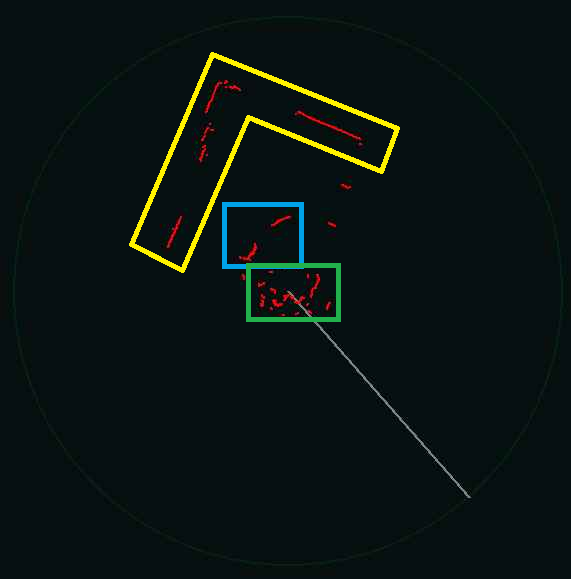
\includegraphics[width=0.4\textwidth, center]{img/LiDARMessungZeichnung_alt.png}
    \caption{LiDAR-Messung}
    \label{fig:LiDAR-Messung}
\end{figure}
Das Bild zeigt die generierte Punktwolke des LiDAR-Sensors. Die Punktwolke zeigt ideal die Funktionsweise des LiDARs und ist leicht zu interpretieren. 
Die unterschiedlichen Laserimpulse, welche gesendet werden, reflektieren an der Oberfläche und werden gemessen. Nicht nur ist die Entfernung, sondern auch die Tiefenwahrnehmung somit feststellbar.

Um die Punktwolke genauer zu verstehen, wurden Sektionen eingezeichnet. 
Die Grüne Sektion zeigt Objekte, welche unmittelbar vor dem LiDAR standen, in dem Fall waren es Büromaterialien wie etwa Kugelschreiber, Hefte, etc.
Die blaue Sektion befindet sich ca. 1-2 m vom LiDAR entfernt. Die aufgenommenen Punkte sind einfach nur eine Person sowie ein Sessel.
Die gelbe Sektion war ca. 3 m entfernt und zeigt die Umrandung des Raumes, interessanterweise sind die Lücken die Fenster, wo die Laserimpulse nicht reflektiert worden sind
und somit konnten keine Punkte an der Stelle der Wolke generiert werden konnten.

\subsection{Fernüberwachung per Kamera}
\label{subsec:frontend_cam_stream}
Auf allen drei Robotern befinden sich fest montierte ESP32-Kameras zur Überwachung, welche auf dem Frontend, der Webseite gestreamet werden.
Die Kameras dienen vor allem nur der Überwachung der Roboter und sollen der Gruppe nur helfen, Gefahren rechtzeitig zu identifizieren, um die Sicherheit des Projektes zu gewährleisten. Eingriffe erfolgen nur sofern die Roboter nicht selbst auf die Gefahr reagieren.
Sollte jedoch ein Fehler bei einem Roboter unterlaufen sein, so können wir mithilfe der Fernsteuerung (Siehe Abschnitt \ref{subsec:frontend_control}) probieren, die Roboter aus der Gefahrenzone zu entfernen.

\subsection{Fernsteuerung}
\label{subsec:frontend_control}
Die Idee der Fernsteuerung wurde aus den Prototypen der Projektwoche aus dem Jahr 2023/2024 übernommen. Diese hatten eine Fernsteuerungsfunktion, die hier in der Diplomarbeit nur in Notfällen oder Testzwecken verwendet wird.  

\subsection{Anzeigen der Sensordaten}
\label{subsec:frontend_sensors}
Die Sensordaten werden alle auf dem Frontend dargestellt und stetig aktualisiert. Die Sensoren, welche die Gruppe verwendet, sind der LiDAR, die Beschleunigungssensoren und die Kompasse.
Der LiDAR erstellt eine Karte mithilfe von einer Punktwolke, um die Hindernisse und Entfernungen feststellen zu können. Für mehr Informationen siehe Abschnitt \ref{subsec:frontend_lidar_map}.
%TODO BILD ÄNDERN
\begin{figure}[H]
    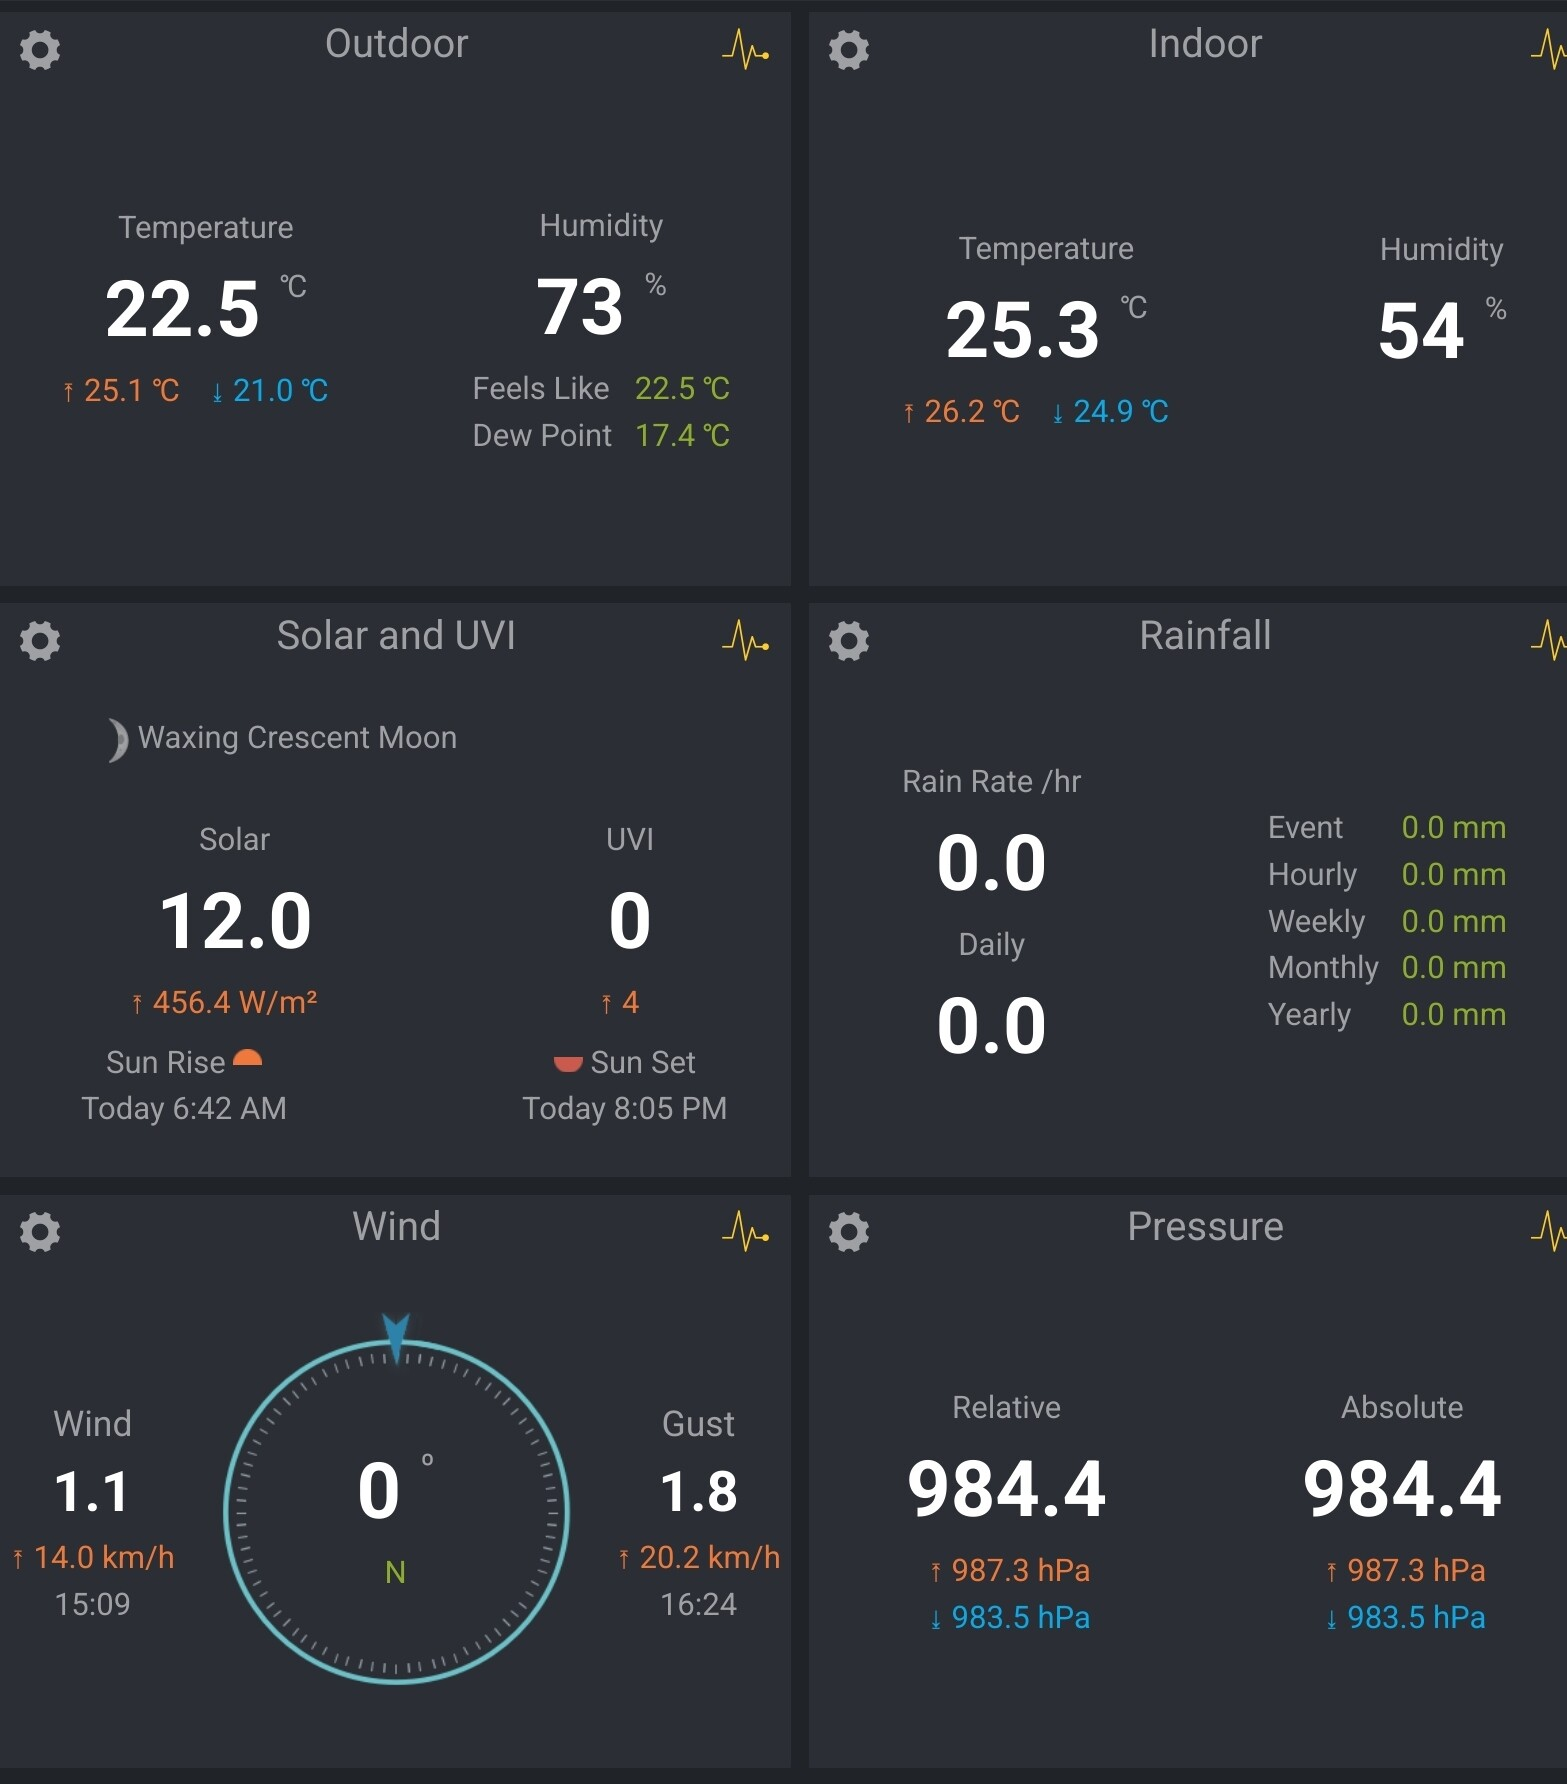
\includegraphics[width=0.4\textwidth, center]{img/Sensor_Anzeige_LOESCHEN.png}
    \caption{Anzeige der Sensordaten}
    \label{fig:Sensordaten}
\end{figure}
Die Beschleunigungssensoren werden in Graphen abhängig von der Zeit angezeigt, um die aktuellen Werte mit den vergangenen Werten vergleichen zu können. Nicht nur werden die Werte in Graphen abgebildet, sondern auch "normal" als Dezimalzahl
um schnell den aktuellsten Wert lesen zu können.
\\
Die Kompasse zeigen die aktuelle Fahrtrichtung der Roboter an. Geplant ist ein "realer" 2D-Kompass, wo die jedoch die Nadel die Fahrtrichtung anzeigt, statt wie gewohnt den Norden.
	% Allgemeine Probleme (Hard- und Software)

\chapter{Probleme}
\label{sec:probleme}
\section{Docker}
\label{subsec:probleme_docker}
\initials{LG}
%TODO wording?
Am Laptop von Herr Gastgeber war es am Beginn des Schuljahres nicht möglich,
jegliche Geräte im Netzwerk der HTL zu erreichen.
%
Grund dafür war eine Software namens Docker,
welche außerhalb dieses Projekts zur Containerisierung von anderen Anwendungen dient.
%
Docker war standardmäßig so konfiguriert,
dass es containerspezifische Subnets im IPv4-Adressbereich \allowbreak\texttt{172.117.0.0/16} erstellt.
%
Diese Subnets hatten dann am Laptop eine höhere Priorität als das Schulnetzwerk,
was dafür sorgte,
dass das weltweite Internet noch erreichbar war, 
nicht aber das lokale Schulnetzwerk.
%
Um Docker einen anderen IP-Adressbereich zuzuweisen,
wurde der Docker-Daemon mithilfe der Datei \texttt{/etc/docker/daemon.json}
wie in Listing \ref{lst:docker_address_pools} konfiguriert.
\begin{lstlisting}[language=json,gobble=4,
    label=lst:docker_address_pools,caption=Konfiguration für den Docker-Daemon]
    {
          "default-address-pools":
          [
            {"base":"10.10.0.0/16","size":24}
          ]
    }
\end{lstlisting}

\section{Modifikationen am Tumbller}
\label{subsec:problem_tumbbler_mods}
\initials{LG}
%TODO kein "wir"
Als wir das Projekt geplant haben,
war die Idee,
einfach ein fertiges Kit ein bisschen zu modifizieren,
fast schon zu schön um wahr zu sein.
%
Und das war es dann auch.
%
Bei den Hardware-Modifikationen am Tumbller (siehe Kapitel \ref{subsec:elegoo_tumbller}) gab es zwei relativ große Probleme:

\subsection{Falsche Betriebsspannungen}
\label{subsec:problem_betriebsspannungen}
\initials{LG}
Beim Austausch des mitgelieferten Arduino Nano mit einem ESP32 im Nano-Format haben wir einen wichtigen Faktor übersehen:
%
Der Arduino Nano hat eine Betriebsspannung von 5V,
während der ESP32 mit 3.3V arbeitet.
%
Glücklicherweise funktionieren die meisten Komponenten des Elegoo Tumbllers auch mit 3.3V.
%
Die einzigen Bauteile,
welche eine höhere Spannung benötigen,
sind die auf der Platine angelöteten farbigen Leuchtdioden.
%
Um nicht das ganze Projekt von Grund auf neu aufbauen zu müssen,
haben wir uns entschieden,
dieses kleine optische Detail fürs Erste auszulassen.
%
%TODO schaltplan
In der originalen Beschaltung (siehe Abbildung \ref{fig:elegoo_tumbller_original_circuit})
wurde das Bluetooth-Modul mithilfe des Spannungswandlers \texttt{U3} mit 3.3V versorgt.
%
Diesen Spannungswandler haben wir ausgebaut und mittels einer Lötbrücke $V_{in}$ mit $V_{out}$ verbunden.
Allerdings erwies sich das Bluetooth Modul später als problematisch (siehe Abschnitt \ref{subsec:problem_bluetooth_serial}),
weshalb die Überbrückung eigentlich nicht notwendig ist.
\\\\
Außerdem war es beim Guide-Roboter aufgrund des Wechsels auf 3.3V nicht mehr möglich,
den LiDAR-Sensor direkt mit dem Spannungswandler des Mikrocontroller-Boards zu versorgen.
%
Deshalb haben wir für den Guide einen zusätzlichen Step-Down-Konverter eingebaut,
welcher die Versorgungsspannung des Akkus auf 5V für den LiDAR herunterregelt.
\section{Blockierte UART-Schnittstelle}
\label{subsec:problem_bluetooth_serial}
\initials{LG}
Als das Problem der inkompatiblen Spannungen gelöst,
und die erste Version des Programmes zum Testen der einzelnen Komponenten geschrieben war,
%TODO Formulierung: "großes Problem" hab ich schon vorher verwendet
sind wir auch schon auf das nächste nennenswerte Problem gestoßen:
%
Das externe Bluetooth-Modul,
was bereits auf der Platine verlötet war,
belegt die UART-Schnittstelle des eingebauten ESP32.
%
Das führte dazu, dass der ESP32 nur neu programmiert werden konnte,
wenn das ESP32-Devboard aus dem Roboter ausgebaut war.
%
Außerdem wurde dadurch das Debuggen mittels UART über USB unmöglich gemacht.
\\
Da wir die Roboter über WLAN steuern,
und der ESP32 auch ohne externe Erweiterungen bereits sowohl über WLAN- als auch Bluetooth-Kapazitäten verfügt,
haben wir entschlossen,
die mitgelieferte Platine weiter zu modifizieren,
indem wir das Bluetooth-Modul entfernen.
%
Außerdem haben wir den Transistor \texttt{Q1} und den Spannungsteiler,
welcher aus \texttt{R9} und \texttt{R10} besteht entfernt,
um sicherzustellen, das die UART-Verbindung keinesfalls beeinflusst wird
(siehe Original-Schaltplan in Abbildung \ref{fig:elegoo_tumbller_original_circuit}).
%TODO Bilder und Erläuterung zu Entfernen des Bluetooth Moduls


\section{Nicht identische Pinbelegung}
% TODO muss überarbeitet werden?
\label{subsec:arduino_to_esp32}
\initials{JS}
Der Wechsel zum ESP32 Nano lief nicht reibungslos wie erhofft da,
obwohl der ESP von Arduino das "gleiche Gehäuse" verwendet 
es jedoch zu einigen Unterschieden in den Pins kommt. 

% TODO änder die pins aufs wichtige
\begin{figure}[H]
    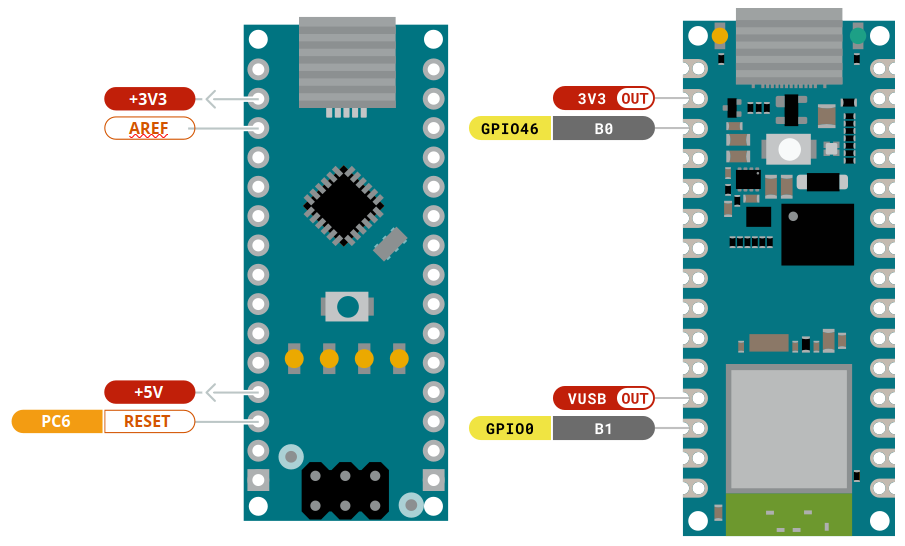
\includegraphics[width=\textwidth, center]{img/nano-differences-m.png}
    \caption{Hervorgehobene Pinbelegung zwischen Arduino und ESP32 nano}
    \label{fig:nano_boards}
\end{figure}

Zwischen den Boards herrschen für dieses Projekt am wesentlichen diese Unterschiede.
\begin{itemize}
    \item Pin 3 von \texttt{AREF} zu \texttt{GPIO46} und \texttt{Boot0}.
    \item Pin 12 von \texttt{+5V} zu \texttt{VUSB} oder \texttt{VBUS}.
    \item Pin 13 von \texttt{RESET} zu \texttt{GPIO0} und \texttt{Boot1}.
\end{itemize}

Der Pin 3 von \texttt{AREF} ist unproblematisch aufgrund dessen dass,
es zu einem ungenutzten I/O Interface führt und somit keinem weiteren Besorgen.

Bei Pin 12 muss etwas Achtung gegeben werden, weil der \texttt{VBUS} im Vergleich zu \texttt{+5V} als
direkte Führung von der Versorgung aus der USB Schnittstelle bedacht wurde und 
dadurch nicht weiter geregelt wird vom Board. Deswegen wird empfohlen den VBUS 
nicht mit anderen Pins am Nano kurz zuschließen, jedoch wenn der ESP32 über den VIN Pin versorgt ist, 
wird der Pin deaktiviert und sollte keine 5V von der USB Schnittstelle liefern können. 
% Weiteres verhalten darüber hinaus ist nicht dokumentiert.
% Mehr dazu und der anderen Betriebsspannung ist in Abschnitt \ref{subsec:problem_betriebsspannungen} zu finden.

Pin 13 sollte keine Probleme machen da es zu einem offenen Schalter geht,
der ursprünglich den \texttt{RESET} Pin betätigt hätte und sonst offen liegt. 
Beim ESP32 würde der Schalter dafür sorgen das zum Boot Mode gewechselt werden kann, 
oder gewöhnliche Operationen mit \texttt{GPIO0}. 
Jedoch kam es zu Störungen an diesem Pin trotz internen Pull-up-Widerstand, 
wodurch wir den Pin entfernt haben mehr dazu siehe Abschnitt \ref{subsec:gestoert_boot}.


\section{Gestörter Boot Prozess} \label{subsec:gestoert_boot}
\initials{JS}
In unseren nächsten Test nachdem wir das Bluetooth-Modul entfernt haben 
und erfolgreich code laden konnten, verweigerte der ESP wieder den Programmierungprozess.
% TODO Bild und erkläarung zu fehlersuche
TODO

Dieser Pin 13 welcher ursprünglich als Reset agierte war nun verantwortlich für GPIO0. 
Jedoch sollte dies keine Probleme bescheren da der Pin offen liegt, weil der Schalter ein Schließer ist,
und nach ESP ein internen Pull-up Widerstand am GPIO0 liegt, kamen es trotzdem zu Störungen.
% https://docs.espressif.com/projects/esptool/en/latest/esp32/advanced-topics/boot-mode-selection.html#gpio0
Daraufhin haben wir den Pin entfernt, um die Störungen komplett zu vermeiden. 
Dies hatte die Folge das bei den Boards wo, die Bluetooth-Module noch nicht entfernt wurden,
jetzt auch neu programmiert werden konnte, ohne jegliche Modifikationen zum Bluetooth-Modul.


	% Abbildungs- und Tabellenverzeichnis
	\newpage
	\appendix
	\addcontentsline{toc}{part}{Anhang}
	\addcontentsline{toc}{chapter}{Abbildungsverzeichnis}
	\listoffigures
	\addcontentsline{toc}{chapter}{Tabellenverzeichnis}
	\listoftables
	\addcontentsline{toc}{chapter}{Literatur}
	\printbibliography
	% Projektmanagment file dropped into the project by Jones Soliman originally created by Mihael Stojkovic
% I have comment out like all the packages and things as can be seen below
% and so far only included \usepackage{longtable} in the preamble 
% as it caused compile errors
% idk if more are needed
% but i can see it's missing in the table of contents
% 'section*' has been replaced with 'subsection'

% \documentclass[a4paper,12pt]{article} ---
% \usepackage[utf8]{inputenc}
% \usepackage[T1]{fontenc}
% \usepackage[ngerman]{babel} --- [german]
% \usepackage{geometry}
% \usepackage{longtable} ---
% \usepackage{array}
% \usepackage{setspace} ---
% \usepackage{booktabs} ---
% \usepackage{hyperref} ---
% \usepackage{ragged2e} % Für bessere Textausrichtung
% \usepackage{lipsum} ---
% \usepackage{float}
% \usepackage{graphicx} % Paket für Grafiken
% \graphicspath{{bilder/}} % Pfad zum Ordner mit den Bildern
% \usepackage{tocbibind} ---

% Seitenränder anpassen
% \geometry{left=25mm, right=25mm, top=30mm, bottom=30mm}

% % Problematisches Verhalten mindern
% \sloppy % Lockert den Textumbruch
% \setlength{\emergencystretch}{3em} % Fügt mehr Flexibilität hinzu

% \title{\textbf{Projekthandbuch \\ SwarmBots}}
% \author{Version 0.3 \\ Projektleiter/in: Mihael Stojkovic \\ Projektteam: Leander Gastgeber, Jones Soliman, Arthur Burjak}
% \date{Datum: 11.01.2025}

% % \begin{document}

% \maketitle
% \tableofcontents
% \newpage
\chapter{Projekthandbuch}
\label{sec:projekthandbuch}

\section{Projektauftrag}
\initials{MS}

% \textbf{PROJEKTAUFTRAG} \\
\textbf{SwarmBots} \\
\textbf{Projektstarttermin:} 02.09.2024 \\
\textbf{Projektendtermin:} 11.04.2025 \\

\textbf{Projektziele:}
\begin{itemize}
    \item Ein Roboter, welcher eine zweidimensionale Karte der Umgebung erstellt und die anderen Roboter leitet („Guide“).
    \item Zwei „blinde“ Roboter („Tamerlan“ und „Bambi“), welche von „Guide“ geleitet werden.
    \item Einen zentralen Server zur Datenverarbeitung, -darstellung und Kommunikation zwischen den Robotern.
\end{itemize}

\textbf{Nicht-Projektziele:}
\begin{itemize}
    \item Entwicklung eines eigenen Antriebssystems für die Roboter.
    \item Bau vieler Roboter.
\end{itemize}

\textbf{Hauptaufgaben:}
\begin{itemize}
    \item Projektmanagement
    \item Software entwickeln
    \item Zusammenbau des Hauptroboters
    \item Modifikation des Hauptroboters
    \item Zusammenbau der Nebenroboter
    \item Modifikation der Nebenroboter
    \item Installation der Basisstation
\end{itemize}

\textbf{Kosten:} Ca. 400 € (zzgl. 120 € von Projektwoche 2024 (LiDAR)) \\

\textbf{ProjektauftraggeberIn:} Erich Erker \\
\textbf{ProjektleiterIn:} Mihael Stojkovic \\
\textbf{Projektteam:} Jones Soliman, Leander Gastgeber, Arthur Burjak \\

\vspace{0,5cm}
\begin{center}
\textbf{Erich Erker (ProjektauftraggeberIn) \\ Mihael Stojkovic (ProjektleiterIn)}
\end{center}

\newpage

\section{Projektzielplan}
\initials{MS}

\textbf{PROJEKTZIELEPLAN} \\

\subsection{Hauptziele}
\initials{MS}
\begin{itemize}
    \item Ein Roboter, welcher eine zweidimensionale Karte der Umgebung erstellt und die anderen Roboter leitet („Guide“), bauen.
    \item Zwei „blinde“ Roboter („Tamerlan“ und „Bambi“), welche von „Guide“ geleitet werden, bauen.
    \item Einen zentralen Server zur Datenverarbeitung, -darstellung und Kommunikation zwischen den Robotern, erstellen.
\end{itemize}

\subsection{Zusatzziele}
\initials{MS}
\begin{itemize}
    \item Balancierung der Roboter auf zwei Rädern entwickeln.
\end{itemize}

\subsection{Nicht-Ziele}
\initials{MS}
\begin{itemize}
    \item Entwicklung eines eigenen Antriebssystems für die Roboter.
    \item Bau vieler Roboter.
\end{itemize}

\newpage

\section{Projektumweltanalyse}
\initials{MS}

\begin{figure}[htbp]
    \centering
    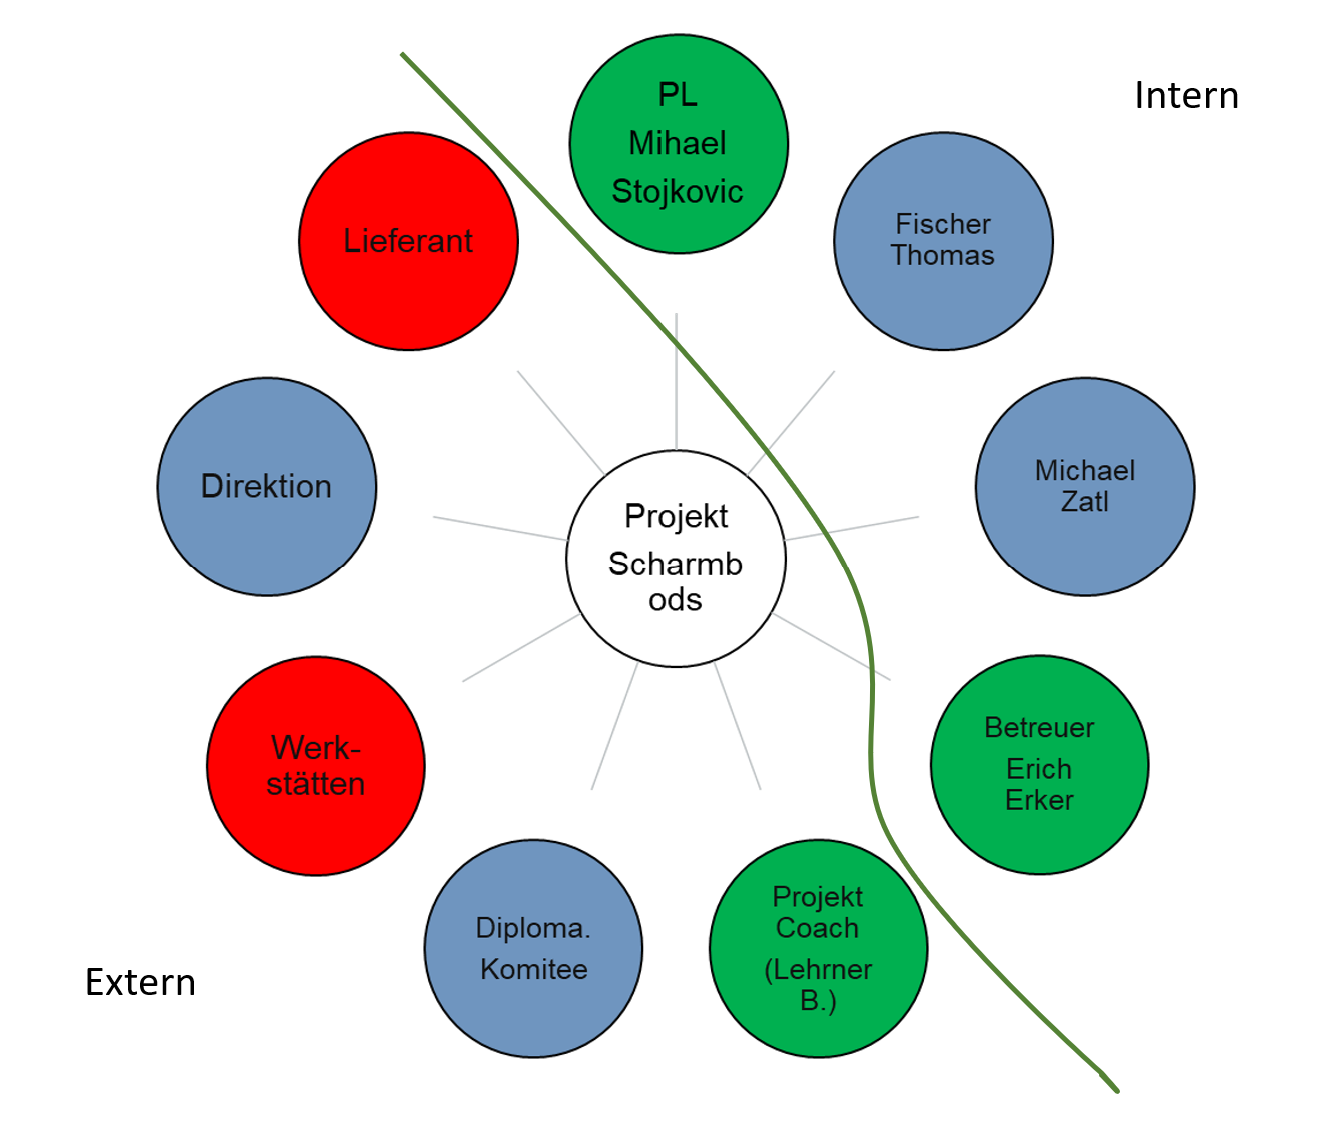
\includegraphics[width=\textwidth]{img/Projektumweltanalyse.png} 
    \caption{}
\end{figure}

\begin{table}[H]
    \centering
    \begin{tabular}{|l|l|l|p{4.5cm}|l|}
        \hline
        \textbf{Nr.} & \textbf{P-Umwelt} & \textbf{Beziehung} & \textbf{Beschreibung} & \textbf{Maßnahmen} \\
        \hline
        1 & Lieferant & - & Evtl. Lieferverspätungen & Frühe Bestellungen \\
        \hline
        2 & Werkstätten & - & Notwendige Ressourcen evtl. nicht vorhanden & Rechtzeitige Anfragen \\
        \hline
    \end{tabular}
    \caption{Projektumwelten}
    \label{tab:projektumwelten}
\end{table}

\newpage

\section{Projektorganigramm}
\initials{MS}

\begin{figure}[H]
    \centering
    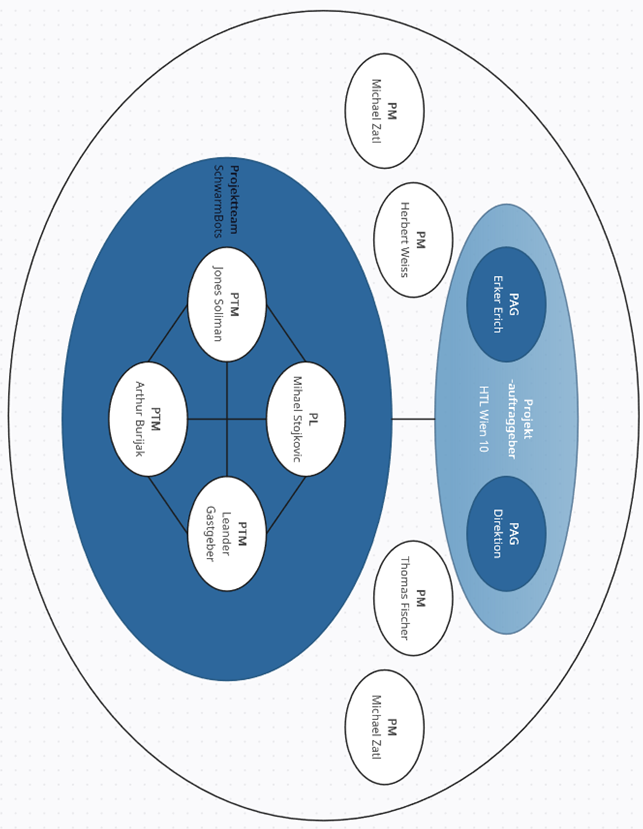
\includegraphics[width=\textwidth]{img/Projektorganigramm.png}
    \caption{Projektorganigramm}
    \label{fig:organigramm}
\end{figure}


\newpage

\section{Projektobjektplan}
\initials{MS}

\begin{figure}[H]
    \centering
    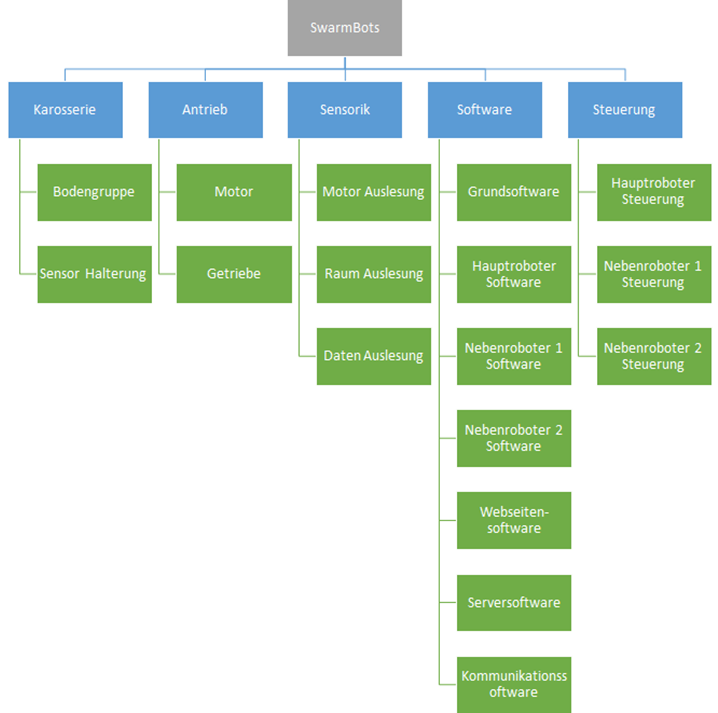
\includegraphics[width=\textwidth]{img/Projektobjektplan.png} 
    \caption{}
\end{figure}

\newpage

\section{Projektstrukturplan}
\initials{MS}

\begin{figure}[H]
    \centering
    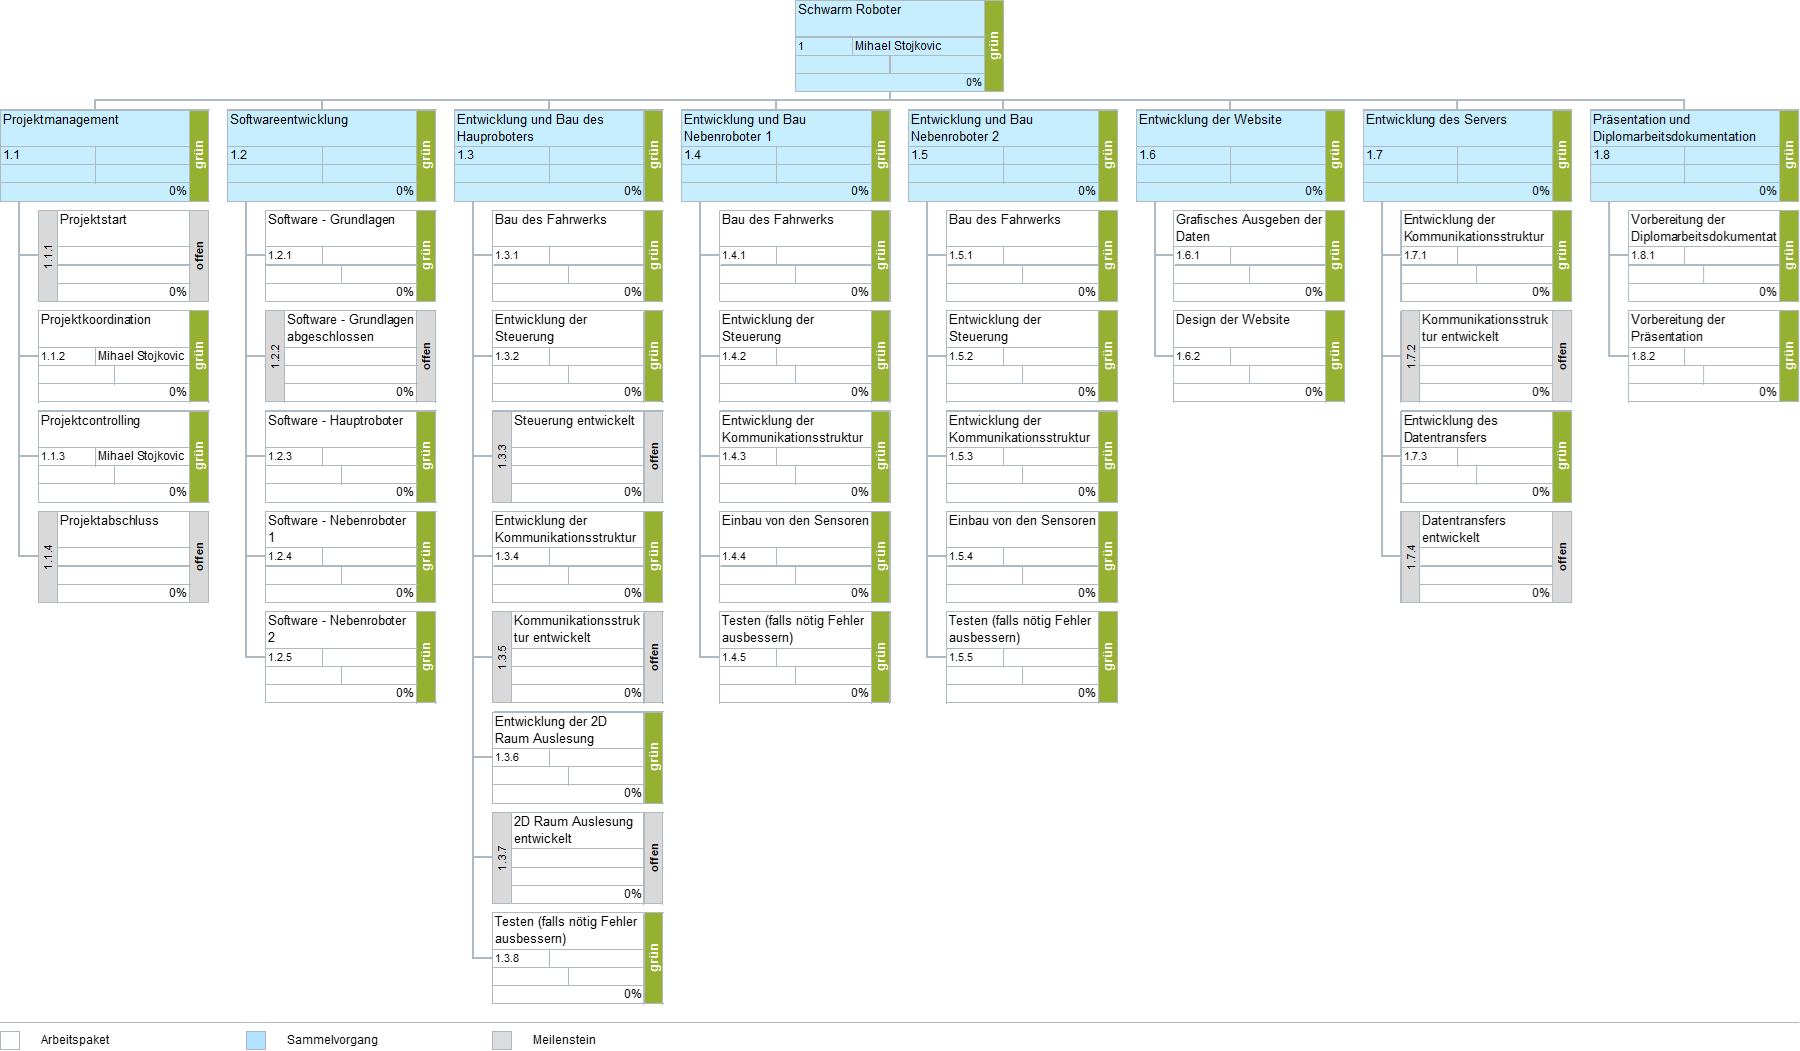
\includegraphics[width=1.4\textwidth, angle=-90]{img/Projektstrukturplan.png}
    \caption{Projektstrukturplan}
    \label{fig:psp}
\end{figure}

\newpage

\section{Projektarbeitspaketspezifikation}
\initials{MS}

\begin{longtable}[c]{|p{1cm}|p{5cm}|p{5cm}|l|}
\hline
\textbf{PSP} & \textbf{Bezeichnung} & \textbf{Inhalt} & \textbf{Verantwortlicher} \\
\hline
1.1.1 & Projektstart & Projektstart vorbereiten, Rahmenbedingungen klären, Projektplan erstellen & Mihael Stojkovic \\
\hline
1.1.2 & Projektkoordination & Aufgaben koordinieren, Fortschritt überwachen & Mihael Stojkovic \\
\hline
1.1.3 & Projektcontrolling & Zeit-, Kosten- und Ressourcenüberwachung & Mihael Stojkovic \\
\hline
1.1.4 & Projektabschluss & Abschlussbericht erstellen, Projekterfolg bewerten & Mihael Stojkovic \\
\hline
1.2.1 & Software - Grundlagen & Gemeinsame Softwarestruktur entwickeln & Leander Gastgeber \\
\hline
1.2.3 & Software - Hauptroboter & LiDAR-Software zur Umgebungserkennung entwickeln & Leander Gastgeber \\
\hline
1.2.4 & Software - Nebenroboter 1 & Sensorauslese-Software entwickeln & Jones Soliman \\
\hline
1.2.5 & Software - Nebenroboter 2 & Sensorauslese-Software entwickeln & Jones Soliman \\
\hline
1.3.1 & Bau des Fahrwerks & Fahrgestell fertigen und montieren & Mihael Stojkovic \\
\hline
1.3.2 & Entwicklung der Steuerung & Autonome Steuerung und manuelle Kontrolle entwickeln & Mihael Stojkovic \\
\hline
1.3.4 & Entwicklung der Kommunikationsstruktur & Protokolle definieren, Kommunikationswege aufbauen & Jones Soliman \\
\hline
1.3.6 & Entwicklung der 2D Raum Auslesung & LiDAR-Daten verarbeiten und vereinheitlichen & Leander Gastgeber \\
\hline
1.3.8 & Testen & Funktionalität testen, Fehler beheben & Arthur Burjak \\
\hline
1.4.1 & Bau des Fahrwerks & Fahrgestell für Nebenroboter fertigen & Mihael Stojkovic \\
\hline
1.4.2 & Entwicklung der Steuerung & Steuerungssoftware für autonomen Nebenroboter entwickeln & Mihael Stojkovic \\
\hline
1.4.3 & Entwicklung der Kommunikationsstruktur & Sensoren einbauen und Software integrieren & Arthur Burjak \\
\hline
1.4.4 & Einbau von den Sensoren & Einbau der Sensoren in den Roboter & Arthur Burjak \\
\hline
1.4.5 & Testen & Verbesserung oder Fehlerkorrektur & Arthur Burjak \\
\hline
1.5.1 & Bau des Fahrwerks & Fertigung und Bau des Fahrgestells & Mihael Stojkovic \\
\hline
1.5.2 & Entwicklung der Steuerung & Entwicklung der Software zum selbständigen Fahren und Steuern des Roboters & Mihael Stojkovic \\
\hline
1.5.3 & Entwicklung der Kommunikationsstruktur & Definition der Protokolle und Datenpakete & Jones Soliman \\
\hline
1.5.4 & Einbau von den Sensoren & Einbau der Sensoren in den Roboter & Arthur Burjak \\
\hline
1.5.5 & Testen & Verbesserung oder Fehlerkorrektur & Arthur Burjak \\
\hline
1.6.1 & Grafisches Ausgeben der Daten & Entwicklung der 2D-Karte mithilfe der LiDAR-Daten & Arthur Burjak \\
\hline
1.6.2 & Design der Website & Programmieren des Designs der Website & Mihael Stojkovic \\
\hline
1.7.1 & Entwicklung der Kommunikationsstruktur & Definition der Protokolle und Datenpakete (Server zur Website) & Jones Soliman \\
\hline
1.7.3 & Entwicklung des Datentransfers & Definition der Protokolle und Datenpakete (Server zum Roboter) & Leander Gastgeber \\
\hline
1.8.1 & Vorbereitung der Diplomarbeitsdokumentation & Unterlagen für die Dokumentation erstellen und verbessern & Arthur Burjak \\
\hline
1.8.2 & Vorbereitung der Präsentation & Präsentation vorbereiten & Arthur Burjak \\
\hline
\end{longtable}


\newpage

\section{Projektfunktionendiagramm}
\initials{MS}

\begin{longtable}[c]{|p{4,3cm}|p{1cm}|p{1cm}|p{1cm}|p{1cm}|p{1cm}|p{1cm}|p{1cm}|p{1,5cm}|}
\hline
\textbf{Arbeitspakete  /  Phasen} & \textbf{PAG (EE)} & \textbf{PL (MS)} & \textbf{PTM (LG)} & \textbf{PTM (JS)} & \textbf{PTM (AB)} & \textbf{PM (MZ)} & \textbf{PM (BL)} & \textbf{Kunde (HTL)} \\
\hline
Projektmanagement & & & & & & & & \\
\hline
Projektstart & E & D & M & M & M & I & & M \\
\hline
Projektkoordination & & D & M & M & M & I & & \\
\hline
Projektcontrolling & I & D & M & M & M & I & & M \\
\hline
Projektabschluss & M & D & M & M & M & I & & \\
\hline
Softwareentwicklung & & & & & & & & \\
\hline
Software - Grundlagen & & M & D & M & M & I & & \\
\hline
Software - Hauptroboter & & M & D & M & M & I & & \\
\hline
Software - Nebenroboter 1 & & M & D & M & M & I & & \\
\hline
Software - Nebenroboter 2 & & M & D & M & M & I & & \\
\hline
Entwicklung und Bau des Hauptroboters & & & & & & & & \\
\hline
Bau des Fahrwerks & & D & M & M & M & I & & I \\
\hline
Entwicklung der Steuerung & & M & D & M & M & I & & \\
\hline
Entwicklung der Kommunikationsstruktur & I & M & M & D & M & & I & \\
\hline
Entwicklung der 2D Raum Auslesung & & M & D & M & M & I & & \\
\hline
Testen (falls nötig Fehler ausbessern) & & D & M & M & M & & I & \\
\hline
Entwicklung und Bau Nebenroboter 1 & & & & & & & & \\
\hline
Bau des Fahrwerks & & D & M & M & M & & & I \\
\hline
Entwicklung der Steuerung & & M & D & M & M & & & \\
\hline
Entwicklung der Kommunikationsstruktur & I & M & M & D & M & & & \\
\hline
Einbau von den Sensoren & & M & D & M & M & I & & \\
\hline
Testen (falls nötig Fehler ausbessern) & & D & M & M & M & & & \\
\hline
Entwicklung und Bau Nebenroboter 2 & & & & & & & & \\
\hline
Bau des Fahrwerks & & D & M & M & M & & & I \\
\hline
Entwicklung der Steuerung & & M & D & M & M & & & \\
\hline
Entwicklung der Kommunikationsstruktur & I & M & M & D & M & & & \\
\hline
Einbau von den Sensoren & & M & D & M & M & I & & \\
\hline
Testen (falls nötig Fehler ausbessern) & & D & M & M & M & & & \\
\hline
Entwicklung der Website & & & & & & & & \\
\hline
Grafisches Ausgeben der Daten & & M & M & M & D & & & \\
\hline
Design der Website & & M & M & M & D & & & \\
\hline
Entwicklung des Servers & & & & & & & & \\
\hline
Entwicklung der Kommunikationsstruktur & I & M & M & D & M & & & \\
\hline
Kommunikationsstruktur entwickelt & I & M & M & D & M & & & \\
\hline
Entwicklung des Datentransfers & & M & M & D & M & & & \\
\hline
Präsentation und Diplomarbeitsdokumentation & & & & & & & & \\
\hline
Vorbereitung der Diplomarbeitsdokumentation & E & M & M & M & D & & & \\
\hline
Vorbereitung der Präsentation & I & M & M & M & D & & & \\
\hline
Präsentieren & E & M & M & M & D & & & \\
\hline
\end{longtable}

\newpage
\section{Projektmeilensteinplan}
\initials{MS}

\begin{longtable}[c]{|p{3cm}|p{6cm}|p{3cm}|l|}
\hline
\textbf{PSP-Code} & \textbf{Meilensteinbezeichnung} & \textbf{Plantermin} & \textbf{Isttermin} \\
\hline
1.1.1 & Projektstart & 02.09.2024 & 02.09.2024 \\
\hline
1.2.2 & Software - Grundlagen abgeschlossen & 25.10.2024 & 25.10.2024 \\
\hline
1.3.3 & Steuerung entwickelt & 20.12.2024 & \\
\hline
1.3.5 & Kommunikationsstruktur entwickelt & 20.12.2024 & \\
\hline
1.3.7 & 2D Raum Auslesung entwickelt & 10.01.2025 & \\
\hline
1.7.2 & Kommunikationsstruktur entwickelt & 10.01.2025 & \\
\hline
1.7.4 & Datentransfers entwickelt & 31.01.2025 & \\
\hline
1.1.4 & Projektabschluss & 11.04.2025 & \\
\hline
\end{longtable}

\newpage

\section{Projektbalkenplan}
\initials{MS}

\begin{figure}[htbp]
    \centering
    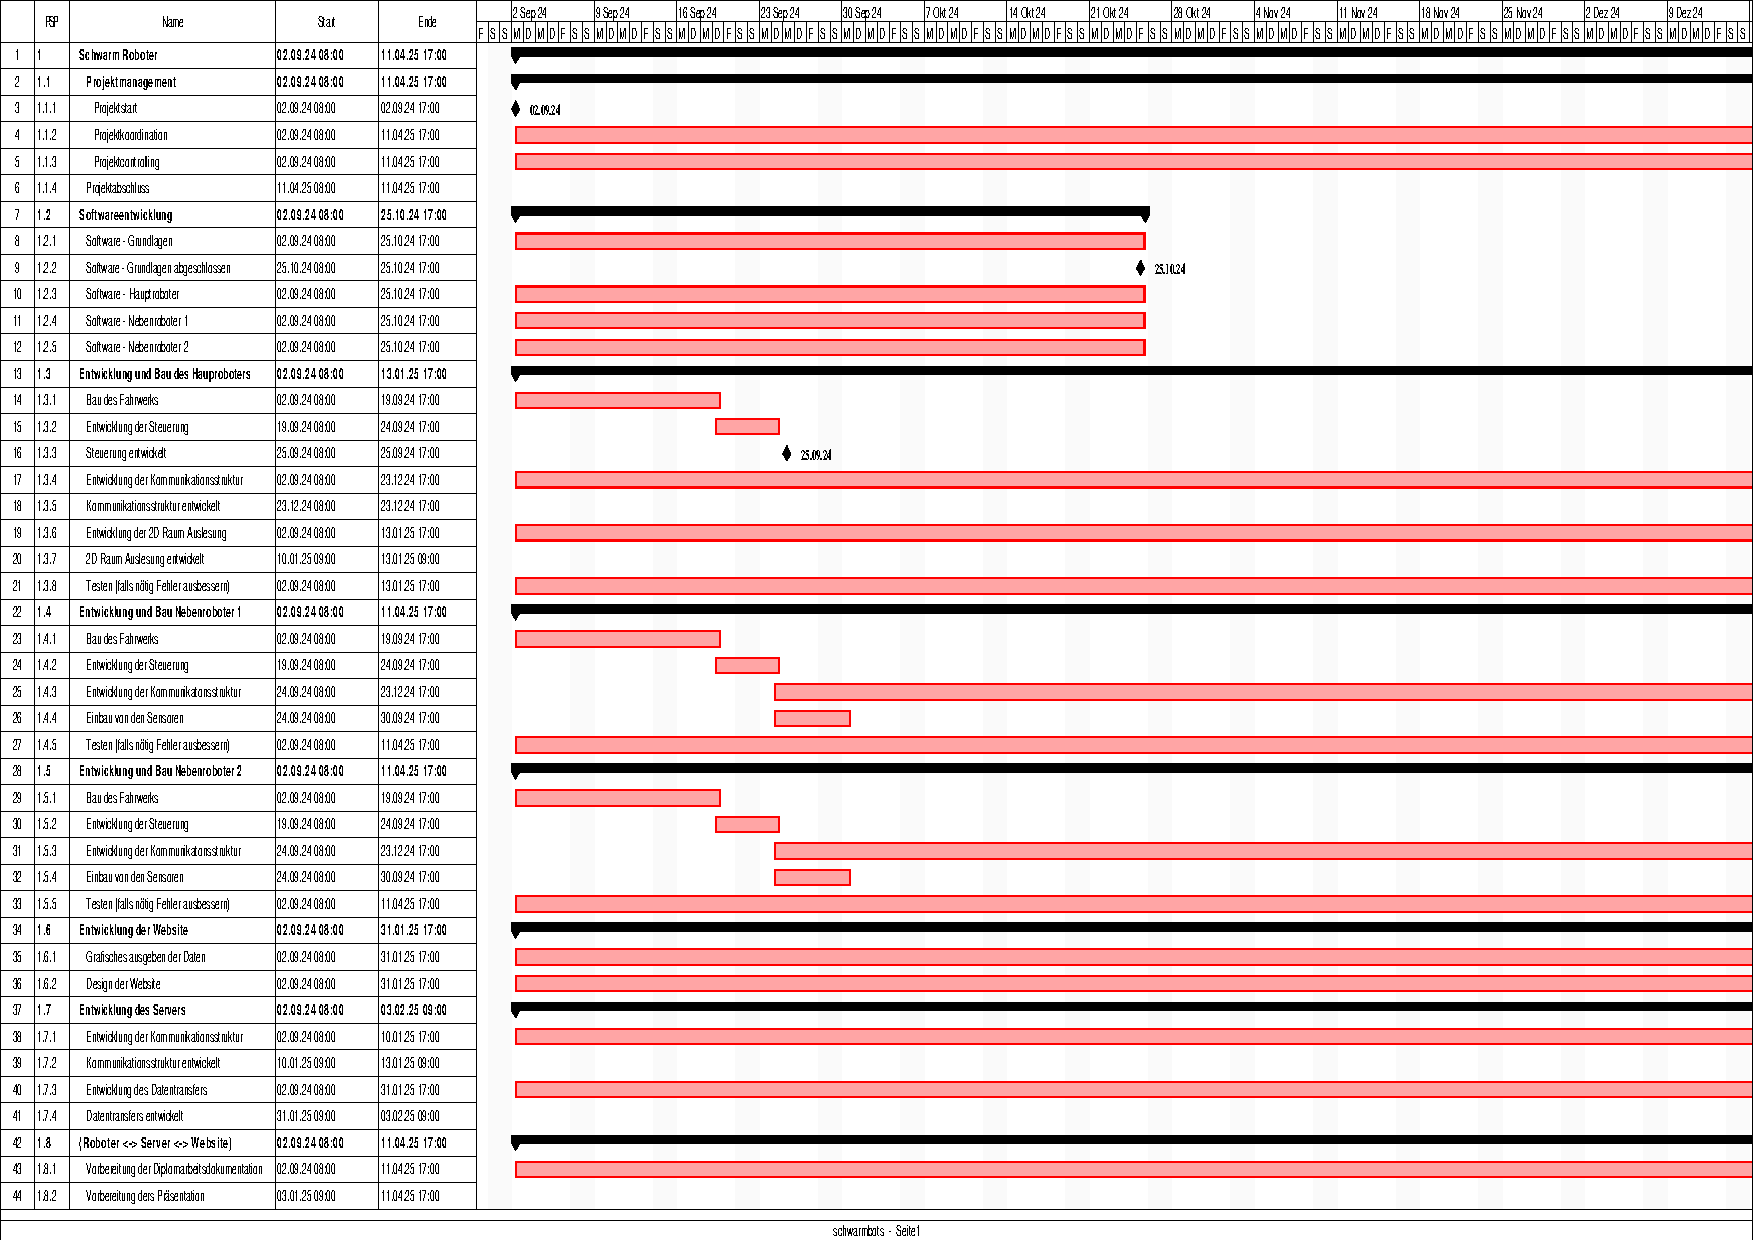
\includegraphics[width=1.2\textwidth,page=1,angle=-90]{img/Projektbalkenplan-gantt_landscape.pdf}
    \label{fig:psp_balk}
\end{figure}
\begin{figure}[htbp]
    \centering
    \includegraphics[width=1.2\textwidth,page=2,angle=-90]{img/Projektbalkenplan-gantt_landscape.pdf}
    \label{fig:psp_balk2}
\end{figure}
\newpage

\section{Projektkostenplan}
\initials{MS}

\begin{longtable}[c]{|p{0,8cm}|p{3cm}|p{1,9cm}|p{1,9cm}|p{2cm}|p{1,9cm}|p{1,9cm}|}
\hline
\textbf{PSP} & \textbf{Arbeitspaket} & \textbf{Personal (€)} & \textbf{Material (€)} & \textbf{Fremd-  leistung (€)} & \textbf{Sonstige (€)} & \textbf{Gesamt (€)} \\
\hline
1.1.1 & Start-Prozess & 2500 & 0 & 350 & 0 & 2850 \\
\hline
1.1.2 & Projektkoordi- nation & 2500 & 0 & 350 & 0 & 2850 \\
\hline
1.1.3 & Projektcontro- lling & 2500 & 0 & 350 & 0 & 2850 \\
\hline
1.1.4 & Projektabschluss-Prozess & 2500 & 0 & 350 & 0 & 2850 \\
\hline
1.2.1 & Software - Grundlagen & 1250 & 0 & 0 & 0 & 1250 \\
\hline
1.2.2 & Software - Grundlagen abgeschlossen & 100 & 0 & 0 & 0 & 100 \\
\hline
1.2.3 & Software - Hauptroboter & 1250 & 0 & 0 & 0 & 1250 \\
\hline
1.2.4 & Software - Nebenroboter 1 & 1250 & 0 & 0 & 0 & 1250 \\
\hline
1.2.5 & Software - Nebenroboter 2 & 1250 & 0 & 0 & 0 & 1250 \\
\hline
1.3.1 & Bau des Fahrwerks & 2250 & 90 & 0 & 0 & 2340 \\
\hline
1.3.2 & Entwicklung der Steuerung & 2500 & 0 & 0 & 0 & 2500 \\
\hline
1.3.3 & Steuerung entwickelt & 100 & 0 & 0 & 0 & 100 \\
\hline
1.3.4 & Entwicklung der Kommunikationsstruktur & 2500 & 0 & 0 & 0 & 2500 \\
\hline
1.3.5 & Kommunikations- struktur entwickelt & 100 & 0 & 0 & 0 & 100 \\
\hline
1.3.6 & Entwicklung der 2D Raum Auslesung & 1250 & 150 & 0 & 0 & 1400 \\
\hline
1.3.7 & 2D Raum Auslesung entwickelt & 100 & 0 & 0 & 0 & 100 \\
\hline
1.3.8 & Testen & 2250 & 0 & 0 & 0 & 2250 \\
\hline
1.4.1 & Bau des Fahrwerks & 2250 & 90 & 0 & 0 & 2340 \\
\hline
1.4.2 & Entwicklung der Steuerung & 2500 & 0 & 0 & 0 & 2500 \\
\hline
1.4.3 & Entwicklung der Kommunikationsstruktur & 2500 & 0 & 0 & 0 & 2500 \\
\hline
1.4.4 & Einbau von den Sensoren & 2250 & 50 & 0 & 0 & 2300 \\
\hline
1.4.5 & Testen & 2250 & 0 & 0 & 0 & 2250 \\
\hline
1.5.1 & Bau des Fahrwerks & 2250 & 90 & 0 & 0 & 2340 \\
\hline
1.5.2 & Entwicklung der Steuerung & 2500 & 0 & 0 & 0 & 2500 \\
\hline
1.5.3 & Entwicklung der Kommunikationsstruktur & 2500 & 0 & 0 & 0 & 2500 \\
\hline
1.5.4 & Einbau von den Sensoren & 2250 & 50 & 0 & 0 & 2300 \\
\hline
1.5.5 & Testen & 2250 & 0 & 0 & 0 & 2250 \\
\hline
1.6.1 & Grafisches ausgeben der Daten & 1500 & 0 & 0 & 0 & 1500 \\
\hline
1.6.2 & Design der Website & 1500 & 0 & 0 & 0 & 1500 \\
\hline
1.7.1 & Entwicklung der Kommunikationsstruktur & 1250 & 0 & 0 & 0 & 1250 \\
\hline
1.7.2 & Kommunikations-  struktur entwickelt & 100 & 0 & 0 & 0 & 100 \\
\hline
1.7.3 & Entwicklung des Datentransfers & 1250 & 0 & 0 & 0 & 1250 \\
\hline
1.7.4 & Datentransfers entwickelt & 100 & 0 & 0 & 0 & 100 \\
\hline
1.8.1 & Vorbereitung der Diplomarbeitsdokumentation & 4000 & 0 & 0 & 0 & 4000 \\
\hline
1.8.2 & Vorbereitung der Präsentation & 4000 & 0 & 0 & 0 & 4000 \\
\hline
1.8.3 & Präsentieren & 4000 & 0 & 0 & 0 & 4000 \\
\hline
\end{longtable}

\textbf{Zusätzliche Informationen:} \\
1.3.1 / 1.4.1 / 1.5.1: 90 € für die Roboterkits. \\
1.3.4: 150 € für den LiDAR und ESP32 Nano. \\
1.4.4 / 1.5.4: 50 € für den ESP32 Nano, ESP32 Cam und die Sensoren. \\

\textbf{Gesamtkosten:} 69.270 € (ohne Personalkosten: 520 €).

% \end{document}

	%TODO % Macros to include code from files
% technically this should go into the preamble, but it fits in better here
% THIS REQUIRES SHELL ESCAPE TO BE ENABLED!!
% enable using the latexmk argument: -shell-escape

% Documentation for expl3 Syntax:
% https://texdoc.org/serve/interface3/0
\ExplSyntaxOn

\tl_new:N \l_input_line
\tl_new:N \l_lst_title

% optional input: arguments for \listinputlisting
% mandatory input: find command (MUST NOT include double quotes! use single quotes instead)
\NewDocumentCommand{\LstInputDir}{O{} m} {
  % check if shell escape is enabled
  \sys_if_shell:F {
  % TODO error message
  }
  % Create temp file
  % check if we're using a unix-ish system or windows
  \sys_if_platform_unix:TF
  % Unix version
  {
    % list all files an write the list into a file JobName.tmp
    \sys_shell_now:e {find~..~-type~f~#2~>~\c_sys_jobname_str.tmp}
    % open temp file Jobname.temp
    \ior_open:Nn \g_tmpa_ior {\c_sys_jobname_str.tmp}
    % if the file is empty, don't execute the next block
    \quark_if_no_value:NF \g_tmpa_ior
    {
      % for each line
      \ior_map_variable:NNn \g_tmpa_ior \l_input_line
      {
        % strip "../" from filenames for the listing caption
        \tl_set:Ne \l_lst_title {
          \tl_range:Nnn \l_input_line {4} {-1}
        }

        % underscores are a special character in LaTeX and cause issues when generating list of listings
        %\tl_replace_all:Nen \l_lst_title { \c_underscore_str } { - }
        % ^ TODO this isn't working

        \texttt{\tl_to_str:N \l_lst_title}:
        % include listing (and forward any options)
        \lstinputlisting[caption="{\tl_to_str:N \l_lst_title}",captionpos=below,#1]{\l_input_line}
      }
    }
    % close file
    \ior_close:N \g_tmpa_ior
  
    % Delete temp file
    \sys_shell_now:e {rm~-f~\c_sys_jobname_str.tmp}
    }
    % Windows is not supported because it doesn't have the same find command
    {
      \textcolor{red}{[Windows~ist~nicht~unterstützt.~Um~den~Code~zu~inkludieren,~bitte~ein~Unix-ähnliches~System~(Linux~oder~macOS)~verwenden!]}
    }
}

% shorthand to automatically exclude hidden files and images
\NewDocumentCommand{\LstInputDirIgn}{O{} m} {
  \LstInputDir[#1]{#2~
  -not~-path~'../*/.*'~
  -not~-name~'*.png'~
  -not~-name~'*.jpg'~
  -not~-name~'*.ico'~
  -not~-name~'*.svg'~
  }
}

\ExplSyntaxOff

\chapter{Code}
Es folgt die aktuelle Version der Sourcecodes vom \today.
%TODO \lstlistoflistings

\section{Protocol Buffers}
\label{lstsec:incl-protobuf}
Siehe Abschnitt \ref{subsec:ueberblick_protobufs} auf Seite \pageref{subsec:ueberblick_protobufs}.
\newline
\LstInputDir{-path '../proto/*.proto'}

\section{Commons}
\label{lstsec:incl-commons}
Siehe Abschnitt \ref{subec:robots_core} auf Seite \pageref{subec:robots_core}.
\newline
\LstInputDirIgn{-path '../robots/commons/*'}

\section{Guide}
\label{lstsec:incl-guide}
Siehe Abschnitt \ref{subsec:software_guide} auf Seite \pageref{subsec:software_guide}.
\newline
\LstInputDirIgn{-path '../robots/guide/*'}

% TODO tamerlan und bambi

\section{ESP32-CAM}
\label{lstsec:incl-cam}
Siehe Abschnitt \ref{subsec:robots_cams} auf Seite \pageref{subsec:robots_cams}
\newline
\LstInputDirIgn{-path '../cam/*'}

\section{Server}
\label{lstsec:incl-server}
Siehe Abschnitt \ref{sec:software_backend} auf Seite \pageref{sec:software_backend}.
\newline
\LstInputDirIgn{-path '../server/*.py' -not -path '../server/protobuf/*'}

\section{Frontend}
\label{lstsec:incl-frontend}
Siehe Abschnitt \ref{sec:software_frontend} auf Seite \pageref{sec:software_frontend}.
\newline
\LstInputDirIgn{-path '../frontend/*'
  -not -path '../frontend/node_modules/*'
  -not -path '../frontend/package-lock.json'
  -not -path '../frontend/src/lib/*'
}

% Rekursion :D
\section{LaTeX Code Inclusion}
\label{lstsec:incl-latex}
Da der LaTeX-Code zur vollautomatischen Inklusion der anderen Codes (im Gegensatz zum Rest der LaTeX-Dateien)
technisch anspruchsvoll ist,
ist dieser hier auch inkludiert,
auch wenn er nicht direkt zum Diplomprojekt beiträgt:

\lstinputlisting[caption="\texttt{Code.tex}",captionpos=below]{./Code.tex}
\end{document}